\documentclass[12pt]{article}

\usepackage{polski}
\usepackage[utf8]{inputenc}
\usepackage{graphicx}
\usepackage{xcolor}
\usepackage{float}
\usepackage{caption}
\usepackage{array}
\usepackage{pbox}
\usepackage{amsmath}

\newcommand\tab[1][1cm]{\hspace*{#1}}

\title{Dokumentacja projektowa}
\date{2018-03-18}
\author{Jędrzej Kozal}

\begin{document}

\begin{titlepage}
	\centering
	
\includegraphics[width=0.25\textwidth]{logo_pol_wroclaw.png}\par\vspace{1cm}
	{\scshape\LARGE Politechnika Wrocławska \par}
	\vspace{1cm}
	{\scshape\Large Podstawy Obliczeń Neuronowych\par}
	\vspace{1.5cm}
	{\huge\bfseries Sieci radialne w predykcji procesów medycznych - choroba Parkinsona \par}
	\vspace{2cm}
	{\Large\itshape Filip Guzy\par}
	{\Large\itshape Jędrzej Kozal\par}

	\vfill
	prowadzący\par
	Dr inż.~Edward \textsc{Puchała}

	\vfill

% Bottom of the page
	{\large \today\par}
\end{titlepage}

\tableofcontents
\newpage


\section{Wstęp}

\subsection{Cel projektu}

Celem projektu było zbadanie skuteczności radialnych sieci neuronowych w~predykcji przebiegu choroby Parkinsona.

\subsection{Wykorzystane narzędzia}

Do realizacji projektu wykorzystano środowisko Matlab, w tym Deep Learning Toolbox zawierający funkcje niezbędne do tworzenia radialnych sieci neuronowych oraz dane ze zbioru uczącego UCI Oxford Parkinson's Disease Telemonitoring Dataset, udostępnionego przez autorów do celów naukowo-badawczych \cite{zbioruczacy}. 

\subsection{Aspekt medyczny}

Parkinson jest zwyrodnieniową chorobą ośrodkowego układu nerwowego. Występuje ona najczęściej u osób starszych, głównie mężczyzn i rozwija się przez kilkanaście lat. Jej objawami są między innymi: osłabienie, zmęczenie, spowolnienie ruchowe, drżenie mięśni czy też kłopoty z wykonywaniem codziennych czynności, takich jak wstawanie, mycie, jedzenie, ubieranie się.  Objawy te oraz sposób rozwoju choroby pozwalają na stworzenie systemów predykcyjnych umożliwiających ciągłe monitorowanie stanu zdrowia pacjentów. Zbiór uczący użyty w projekcie wykorzystuje pomiary głosu pacjentów wykonane przez urządzenie telemedyczne służące do śledzenia przebiegu choroby w~sześciomiesięcznym przedziale czasu. Dla pojedynczego pacjenta zawiera on parametry takie jak: identyfikator, wiek oraz płeć, interwały czasowe wykonanych pomiarów, szesnaście parametrów opisujących nagrany dźwięk, a także parametry wynikowe UPDRS (Unified Parkinson's Disease Rating Scale) opisujące postęp choroby. W zbiorze znajdują się dane zawierające informację o 42 różnych pacjentach, po około 140 pomiarów dla pojedynczej osoby, co łącznie daje około 5000 rekordów.

\section{Zarys podstaw teoretycznych}

\subsection{Topologia radialnych sieci neuronowych}

Radialne sieci neuronowe są specjalną odmianą perceptronów wielowarstwowych. Tak jak one realizują bowiem odwzorowanie zbioru wejściowego w~wyjściowy, robią to jednak poprzez dopasowanie wielu pojedynczych funkcji aproksymujących do wartości zadanych. Odwzorowania takie ważne są tylko w wąskim obszarze przestrzeni wielowymiarowej, zatem ich suma jest odwzorowaniem pełnego zbioru danych. Neurony warstwy ukrytej w sieciach radialnych realizują funkcję zmieniającą się radialnie wokół wybranego centrum \textsl{c} i przyjmującą wartości niezerowe jedynie w otoczeniu tego punktu. Realizację taką przedstawia poniższy rysunek:

\begin{figure}[h!]
\centering
	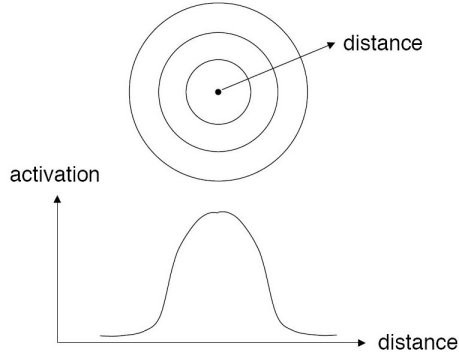
\includegraphics[width=0.5\textwidth]{rbf-gauss.jpeg}\par\vspace{1cm}
\caption{Realizacja funkcji zmieniającej się radialnie}
	\label{fig:features}
\end{figure}

Funkcje takie, nazywane radialnymi funkcjami bazowymi, przyjmują postać: 

\[ \varphi(x) = \varphi(||x-c||) \]

Rolę neuronu ukrytego można zatem sprowadzić do odwzorowania radialnego przestrzeni wokół jednego zadanego punktu lub grupy takich punktów stanowiących klaster. Odwzorowanie całej przestrzeni wielowymiarowej przez neurony warstwy wyjściowej jest więc możliwe dzięki superpozycji sygnałów pochodzących od wszystkich neuronów ukrytych. Dobór liczby neuronów warstwy zależy ściśle od przyjętego błędu, przy czym poszczególne neurony dodawane są iteracyjnie, po jednym neuronie w każdej iteracji, aż do osiągnięcia pożądanego błędu średniokwadratowego. Maksymalna liczba neuronów w~warstwie ukrytej nie może przekroczyć  liczby wektorów podanych na wejście sieci. Typowa sieć radialna jest modelem zawierającym warstwę wejściową przyjmującą sygnały opisywane wektorem wejściowym \textbf{x}, warstwę ukrytą neuronów radialnych oraz warstwę wyjściową złożoną z neuronów liniowych. Przykład takiej topologii przestawiono na poniższym rysunku:

\begin{figure}[h!]
\centering
	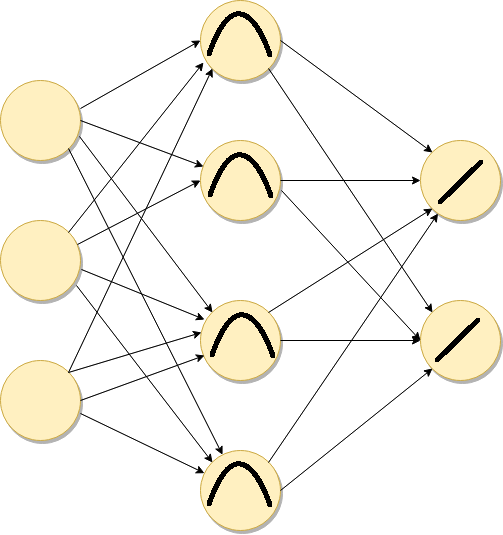
\includegraphics[width=0.5\textwidth]{rbf.png}\par\vspace{1cm}
\caption{Topologia sieci radialnej}
	\label{fig:features}
\end{figure}

\subsection{Wagi neuronów w sieci radialnej}

Przyjmując \textsl{p} neuronów ukrytych połączonych wagami \textsl{$w_i$} z liniowymi neuronami wyjściowymi oraz model sieci radialnej o jednym wyjściu i \textsl{p} parach uczących ($x_i$, $d_i$), a także zakładając \textsl{p} centrów umieszczonych w kolejnych wektorach $x_i$ (tj. $c_i = x_i$) otrzymujemy układ równań liniowych względem wag $w_i$. Układ ten można zapisać w postaci macierzowej:

\[
\begin{bmatrix}
    \varphi_{11}  & \varphi_{12}  & \dots & \varphi_{1p} \\
    \varphi_{21}  & \varphi_{22} &  \dots & \varphi_{2p} \\
    \hdotsfor{4} \\
    \varphi_{p1}  & \varphi_{p2} &  \dots & \varphi_{pp}
\end{bmatrix}
\begin{bmatrix}
	w_1 \\
	w_2 \\
	\dots \\
	w_p
\end{bmatrix}
=
\begin{bmatrix}
	d_1 \\
	d_2 \\
	\dots \\
	d_p
\end{bmatrix}
\]

gdzie:

\[ \varphi_{ji} = \varphi(||x_j-x_i||) \]

dotyczy funkcji radialnej w centrum $x_i$ przy wektorze wymuszającym $x_j$. Oznaczając macierz o elementach $\varphi_{ji}$ jako $\Phi$ i przyjmując oznaczenia wektorów $w = [w_1, w_2, ..., w_p]^T$, $d = [d_1, d_2, ..., d_p]^T$ równanie może być zapisywane w postaci macierzowej:

\[ \Phi w = d \]

Istnieje rozwiązanie równania w postaci:

\[ w = \Phi^{-1} d \]

pozwalające określić wektor wag \textsl{w} neuronu wyjściowego sieci.

\subsection{Algorytmy uczenia sieci radialnych}

Możemy wyróżnić trzy grupy algorytmów uczących mających zastosowanie w procesach uczenia sieci radialnych:

\begin{enumerate}

\item Algorytmy probabilistyczne doboru parametrów funkcji radialnych
\item Algorytmy hybrydowe 
\item Algorytmy oparte na wstecznej propagacji błędu

\end{enumerate}

W projekcie zastosowano algorytm uczenia oparty na mechanizmie wstecznej propagacji błędu. Podobnie jak w sieciach sigmoidalnych, jego podstawę stanowi funkcja celu definiowana dla wszystkich \textsl{p} par neuronów uczących ($x_j$, $d_j$):

\[ E = \frac{1}{2} \sum_{j=1}^{p} [\sum_{i=0}^{K} w_i\varphi_{i}(x_{j} - d_j)]^2 \]

którą to, zakładając jeden wzorzec uczący ($x$, $d$) można uprościć do postaci:

\[ E = \frac{1}{2}  [\sum_{i=0}^{K} w_i\varphi_{i}(x) - d]^2 \]

Należy przyjąć odpowiednie oznaczenia wyjść poszczególnych neuronów:

\begin{flushleft}
$x_m$ - wartość m-tego wejścia \newline
$h_{ij}$ - wartości (i,j) macierzy wyjść neuronów ukrytych, gdzie i - numer warstwy ukrytej, j - numer neuronu w warstwie \newline
$y_p$ - wartość p-tego wyjścia \newline
\end{flushleft}


Zależności pomiędzy warstwami neuronów można przedstawić jako: \newline

\begin{flushleft}
$h_{1j} = f(\sum_{m=1}^{n} w_{mj}x_m)$ \newline
$h_{2j} = f(\sum_{m=1}^{n} w_{mj}h_{1j})$ \newline
... \newline
$h_{nj} = f(\sum_{m=1}^{n} w_{mj}h_{(n-1)j})$ \newline
$y_p = f(\sum_{m=1}^{n} w_{mj}h_{nj})$ \newline
\end{flushleft}

Kolejne kroki algorytmu można opisać następująco:

\begin{enumerate}

\item \textsl{podanie przykładu ze zbioru uczącego na wejście sieci,}

\item \textsl{wyznaczenie wartości wyjść warstwy wyjściowej,}

\item \textsl{obliczenie wektora błędu - różnicy pomiędzy wartościami założonymi, a otrzymanymi,}

\item \textsl{obliczenie sumy kwadratów elementów wektora błędu,}

\item \textsl{sprawdzenie, czy próg błędu został osiągnięty - warunek stopu algorytmu,}

\item \textsl{wykonanie propagacji wstecznej,}

\item \textsl{aktualizacja wag pomiędzy warstwami ukrytą i wejściową, a następnie pomiędzy wejściową i ukrytą.}

\end{enumerate}

\newpage
\section{Zbiór uczący}

\subsection{Opis zawartości zbioru}

Do realizacji zadania wykorzystano zbiór uczący Parkinsons Telemonitoring Data Set dostępny w repozytorium UCI. Zbiór zawiera pomiary głosów pacjentów we wczesnym etapie choroby Parkinsona. Na bazę składa się 5875 próbek pobranych dla 42 pacjentów.

\subsection{Opis parametrów}

Kolumny z danymi pacjentów zawierają kolejno:
\begin{itemize}
	\item id pacjenta
	\item wiek pacjenta
	\item płeć pacjenta (0 - mężczyzna, 1 - kobieta)
	\item czas od zgłoszenia się do testów
	\item UPDRS motoryczny (Unified Parkinson's Disease Rating Scale)
	\item UPDRS całkowity
	\item Jitter(\%), Jitter(Abs), Jitter:RAP, Jitter:PPQ5, Jitter:DDP - pomiary zmiany częstotliwości podstawowej (drganie)
	\item NHR, HNR (Noise to Harmonics Ratio, Harmonic to Noise Ratio) -  Dwa pomiary stosunku zakłóceń do harmonicznych
	\item Shimmer, Shimmer(dB), Shimmer:APQ3, Shimmer:APQ5, Shimmer:APQ11, Shimmer:DDA - pomiary zmiany amplitudy
	\item RPDE - Miara nieliniowej dynamicznej złożoności systemu
	\item DFA - (Detrended Fluctuation Analysis) Parametr opisujący samopodobieństwo sygnału
	\item PPE - Nieliniowa miara wariacji częstotliwości podostawowej
\end{itemize}

\begin{figure}
\centering
	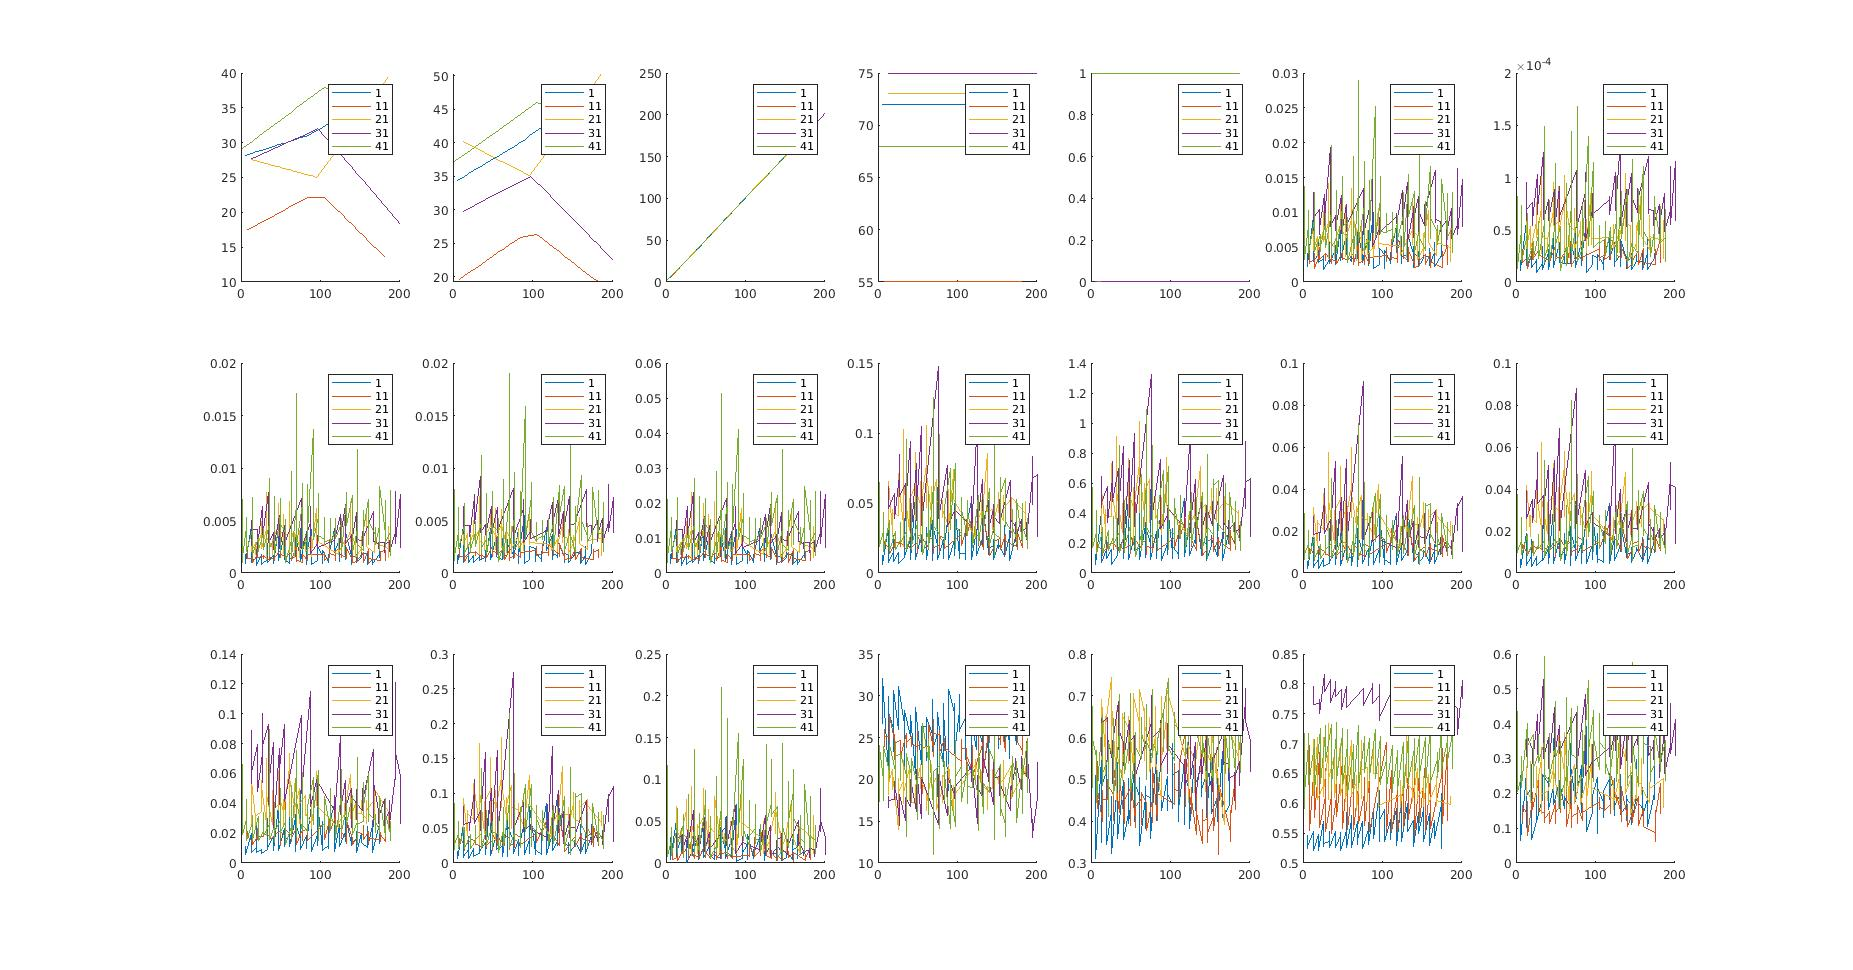
\includegraphics[width=0.90\textwidth]{data.jpg}\par\vspace{1cm}
\caption{Wizualizacja zbioru uczącego}
\label{data visualisation}
\end{figure}

Celem projektu było określenie UPDRS motorycznego na podstawie dostępnych pomiarów  głosów pacjentów. Na rys \ref{data visualisation} przedstawiono zależność wszystkich parametrów od czasu dla pacjentów 1, 11, 21, 31 i 41. Na wykresach 1 i 2 przedstawiono motoryczny i całkowity UPDRS. Na wykresie 3 przedstawiono czas, stąd zaobserwowana zależność liniowa dla wszystkich pacjentów. Na wykresach 4 i 5 przedstawiono wiek i płeć pacjentów - stałe wartości w czasie pomiaru. Na pozostałych wykresach przedstawiono kolejne parametry związane z dźwiękiem wymienione powyżej.

\newpage
\section{Założenia eksperymentu}

\subsection{Podział na zbiór uczący i testowy}
Do zbioru testowego wybrano pierwsze 24 próbki dostępne dla każdego pacjenta. Wszystkie próbki nienależące do zbioru testowego wykorzystano jako zbiór uczący. Liczba wszystkich próbek dostępnych dla i-tego pacjenta nie jest stała, przez co zbiory uczące dla różnych pacjentów zawierały różną liczbę elementów. Minimalna liczba próbek w zbiorze uczącym to 100 próbek dla pojedynczego pacjenta.
 
Przyjęcie takiej metodyki było podyktowane niską liczbą pacjentów w~wykorzystanym zbiorze. Przy 42 pacjentach wydzielenie całych serii pomiarowych wybranych klas zmniejszyłoby zbiór uczący i mogłoby powodować kłopoty z uogólnieniem wyników przez sieć neuronową.

Wszystkie próbki w zbiorze uczącym i testowym zostały posortowane względem czasu w celu ułatwienia analizy uzyskanych wyników.

\subsection{Opis przyjętych metryk}

Do opisu wyników osiągniętych dla zbioru uczącego i testowego wykorzystano błąd średniokwadratowy (MSE). W sprawozdaniu wszystkie wartości MSE dla zbioru uczącego zostały obliczone automatycznie przez Deep Learning Toolbox w środowisku Matlab. W analizowanym zbiorze MSE można je zdefniować jako:

\begin{equation}
 	MSE = \frac{1}{n-1} \sum_{i=1}^{n} \sum_{j=1}^{m_i} (y_{i_j} - F(u_{i_j}))^2
\end{equation}

\begin{flushleft}
 gdzie:\\
 $n$ - liczba pacjentów \\
 $m_i$ - liczba próbek dla i-tego pacjenta \\
 $y_{i_j}$ - oczekiwane wyjście dla i-tego pacjenta i j-tej próbki \\
 $F(u_{i_j})$ - wyjście sieci neuronowej dla i-tego pacjenta i j-tej próbki
\end{flushleft} 


\newpage

\section{Osiągnięte wyniki}
W trakcie przeprowadzania eksperymentu przetestowano sieć neuronową dla czterech konfiguracji:

\begin{enumerate}
\item Dane z duplikatami próbek czasowych z małą ilością pacjentów
\item Dane z duplikatami próbek czasowych z dużą ilością pacjentów
\item Dane bez duplikatów próbek czasowych z małą ilością pacjentów
\item Dane bez duplikatów próbek czasowych z dużą ilością pacjentów
\end{enumerate}

Poniżej omówiono zachowania sieci dla poszczególnych przypadków.

\subsection{Dane z duplikatami próbek czasowych z małą ilością pacjentów}

Parametry uczenia:
\begin{itemize}
\item Mean squared error: $10^{-9}$
\item Spread constant: $10$
\end{itemize}

\begin{figure}[h!]

\centering
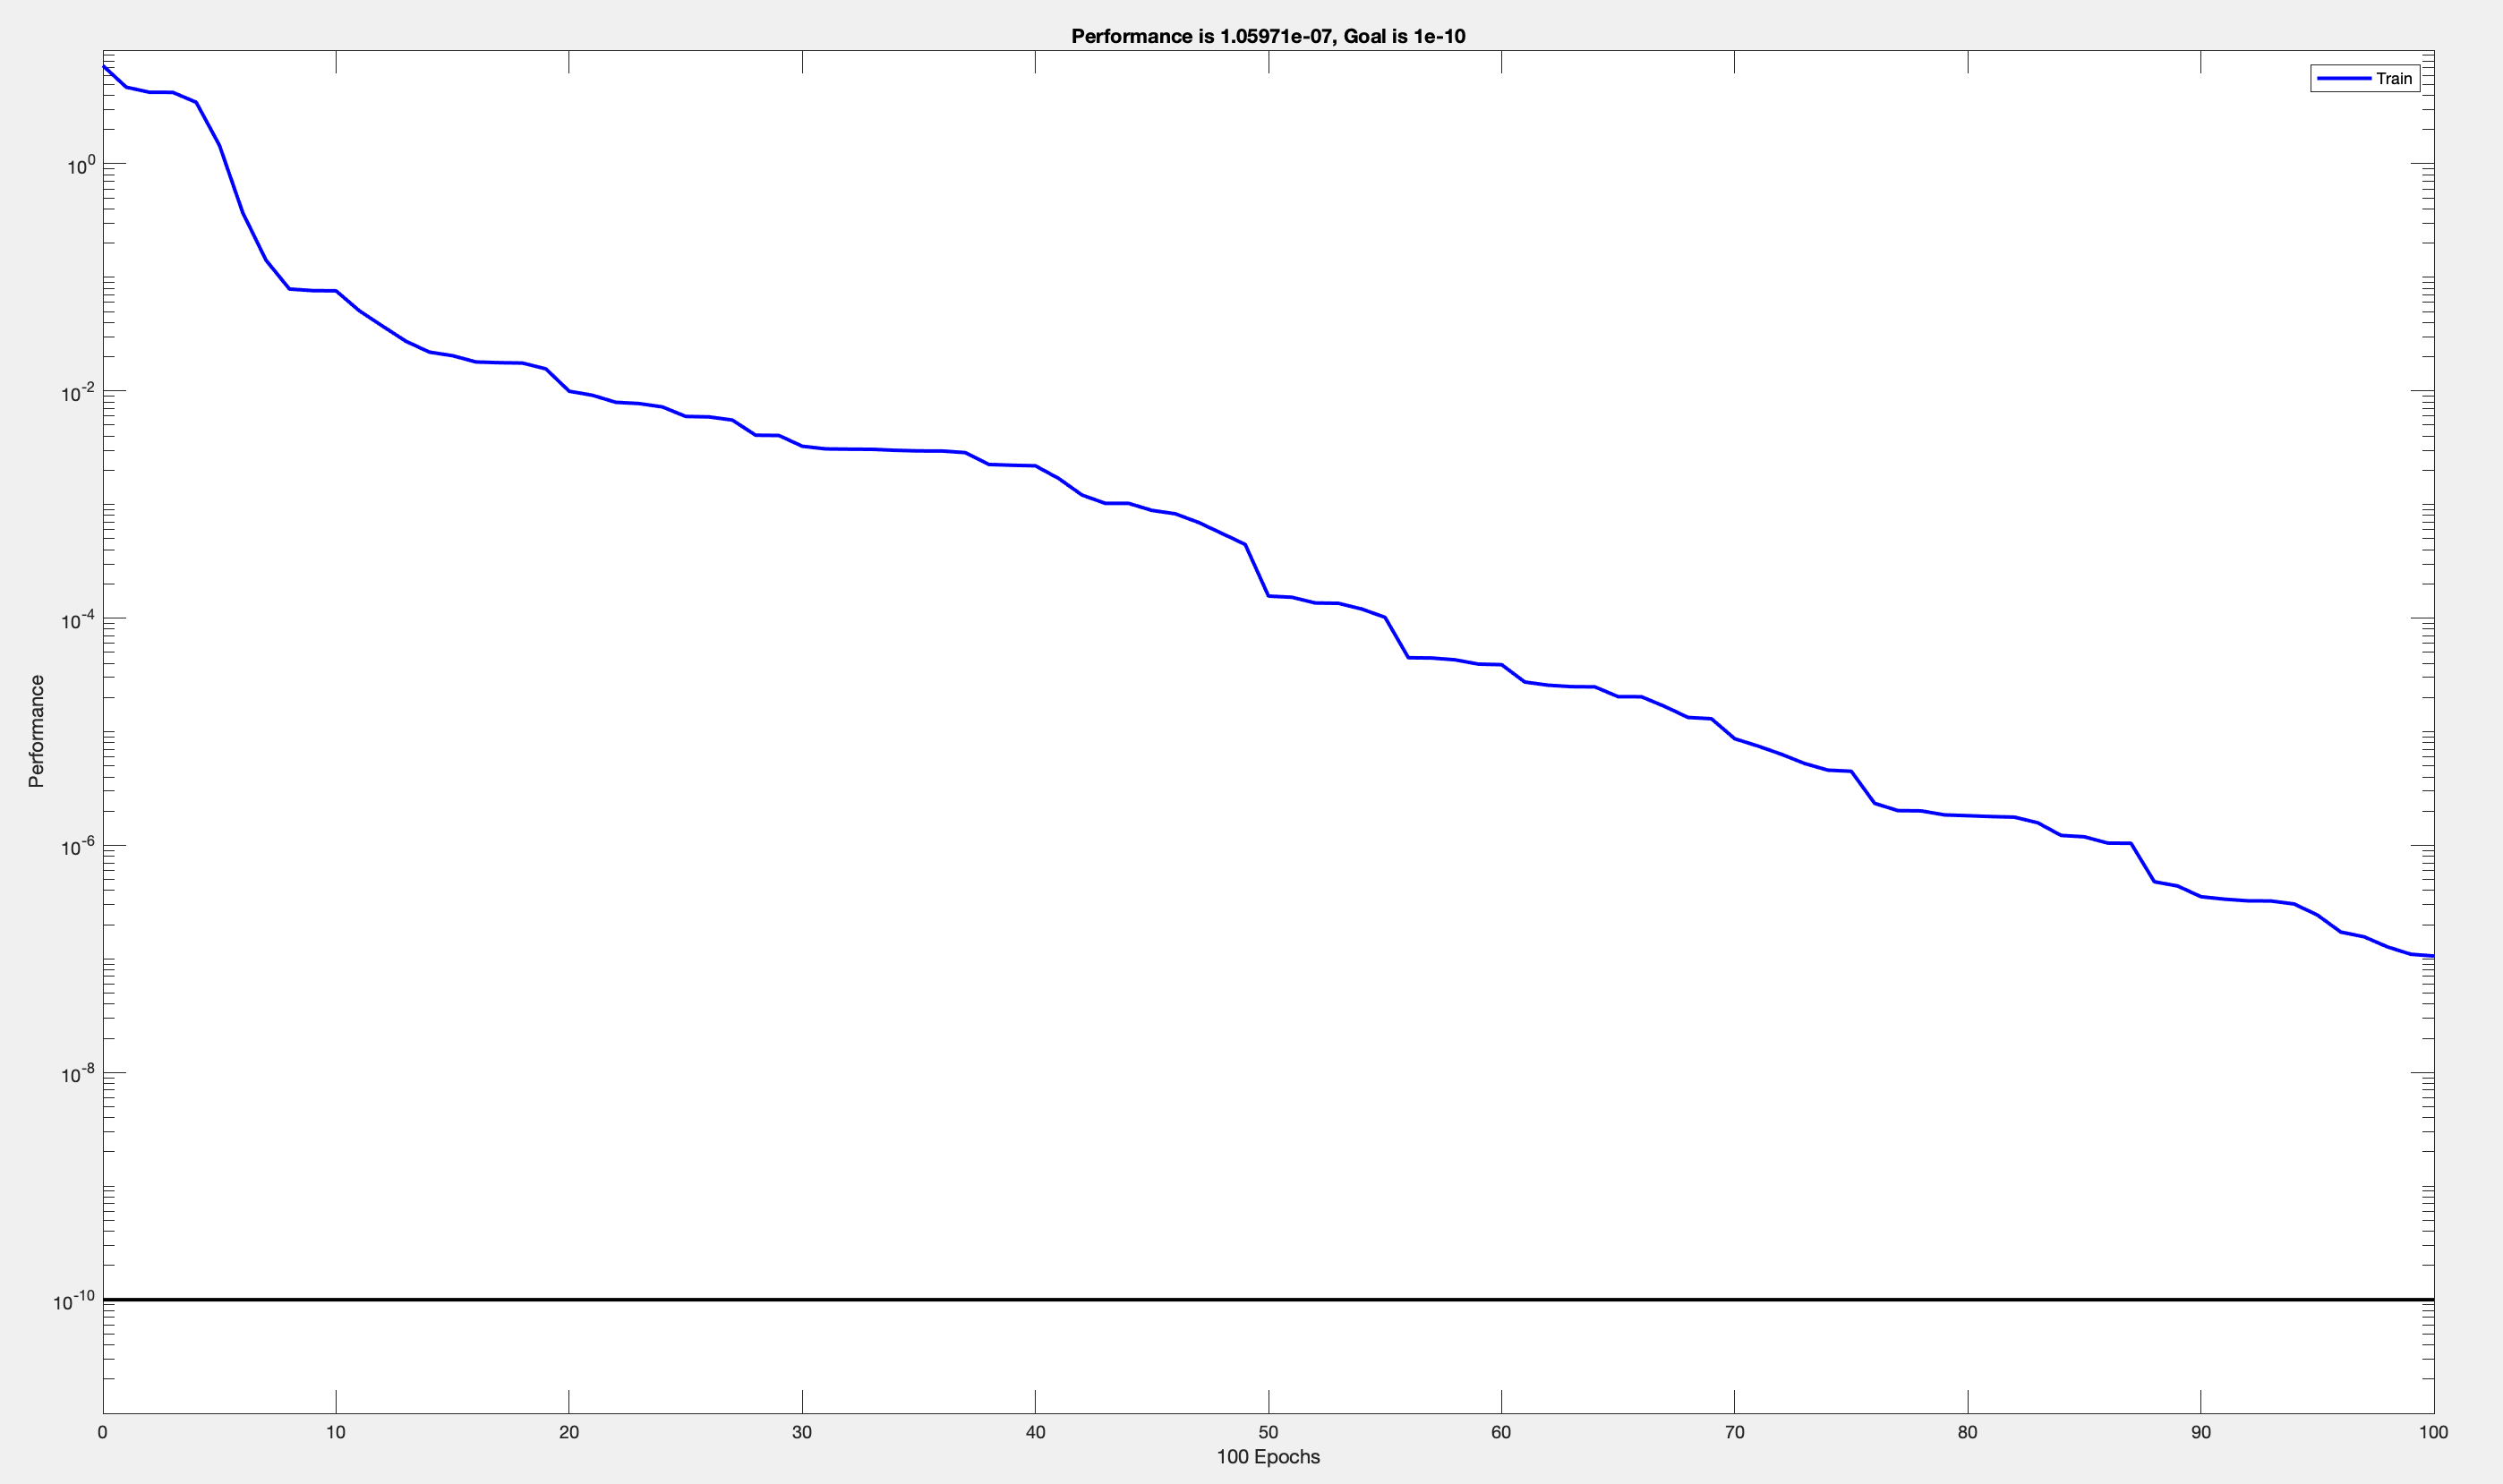
\includegraphics[width=0.8\textwidth]{mse-normal-1.png}
\caption{MSE dla 1 pacjenta}

\end{figure}

\begin{figure}[h!]

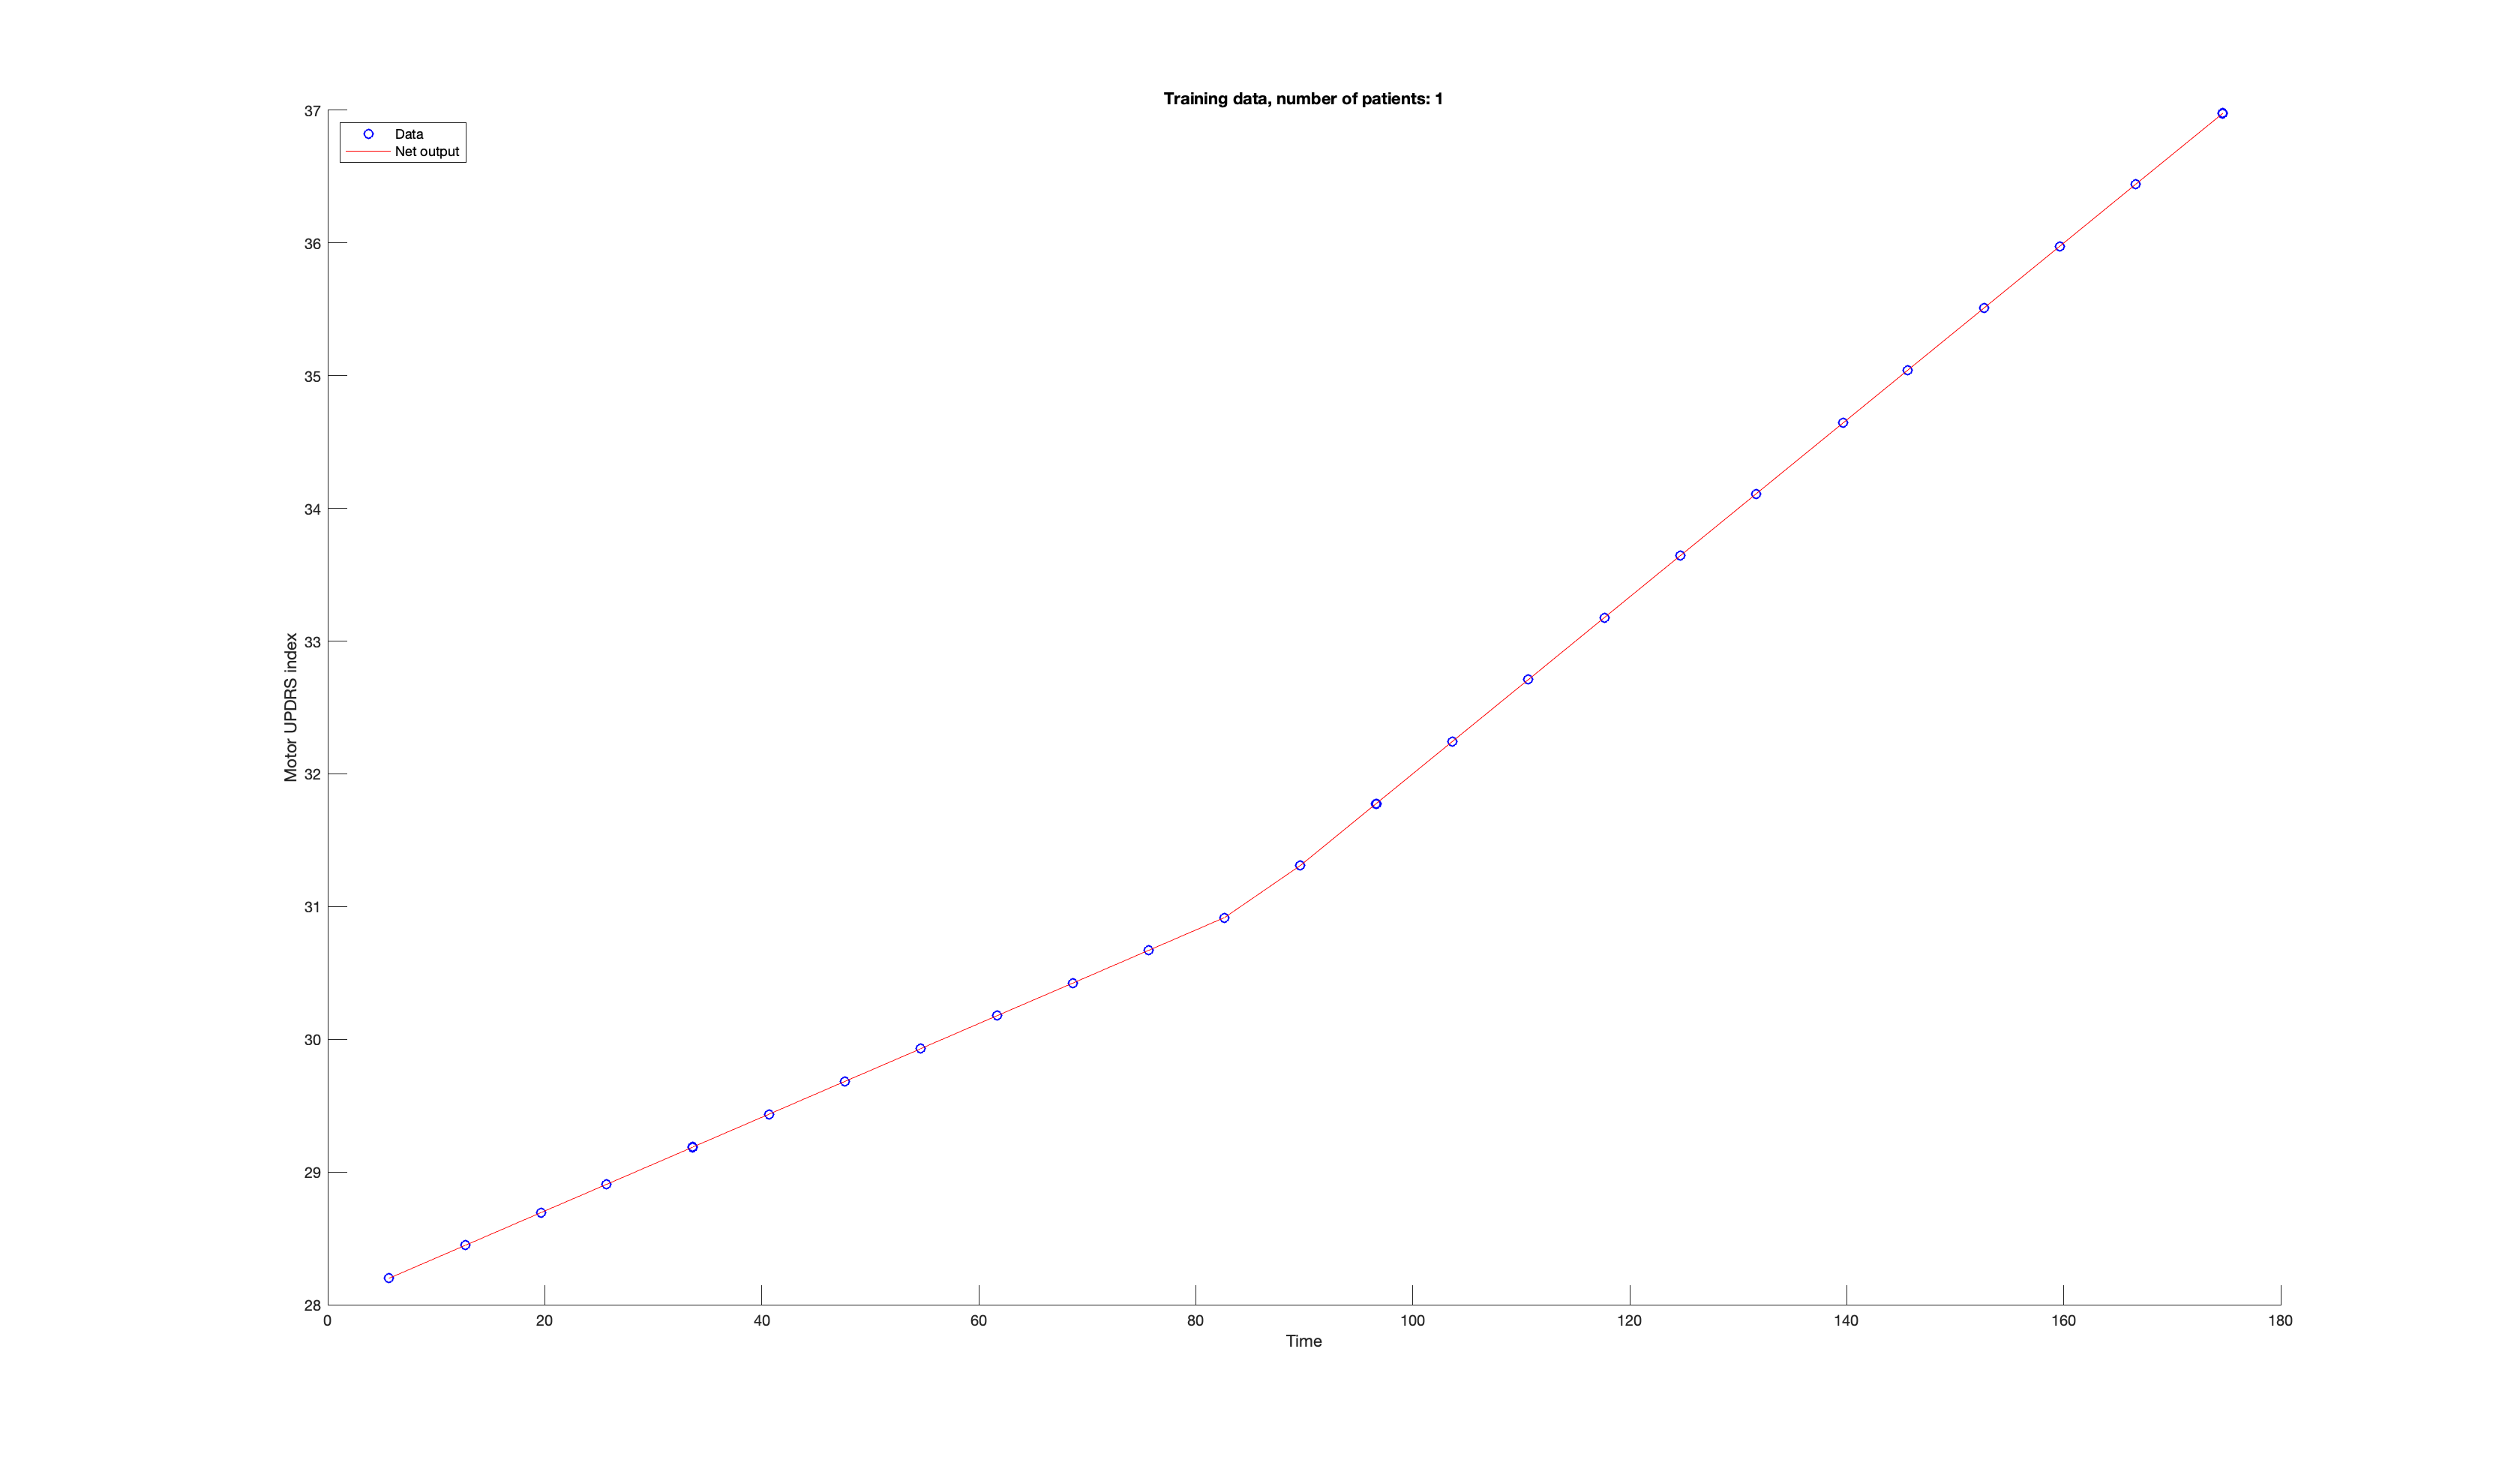
\includegraphics[width=1.05\textwidth]{training-normal-1.png}
\caption{Zbiór treningowy, 1 pacjent}

\end{figure}

\begin{figure}[h!]

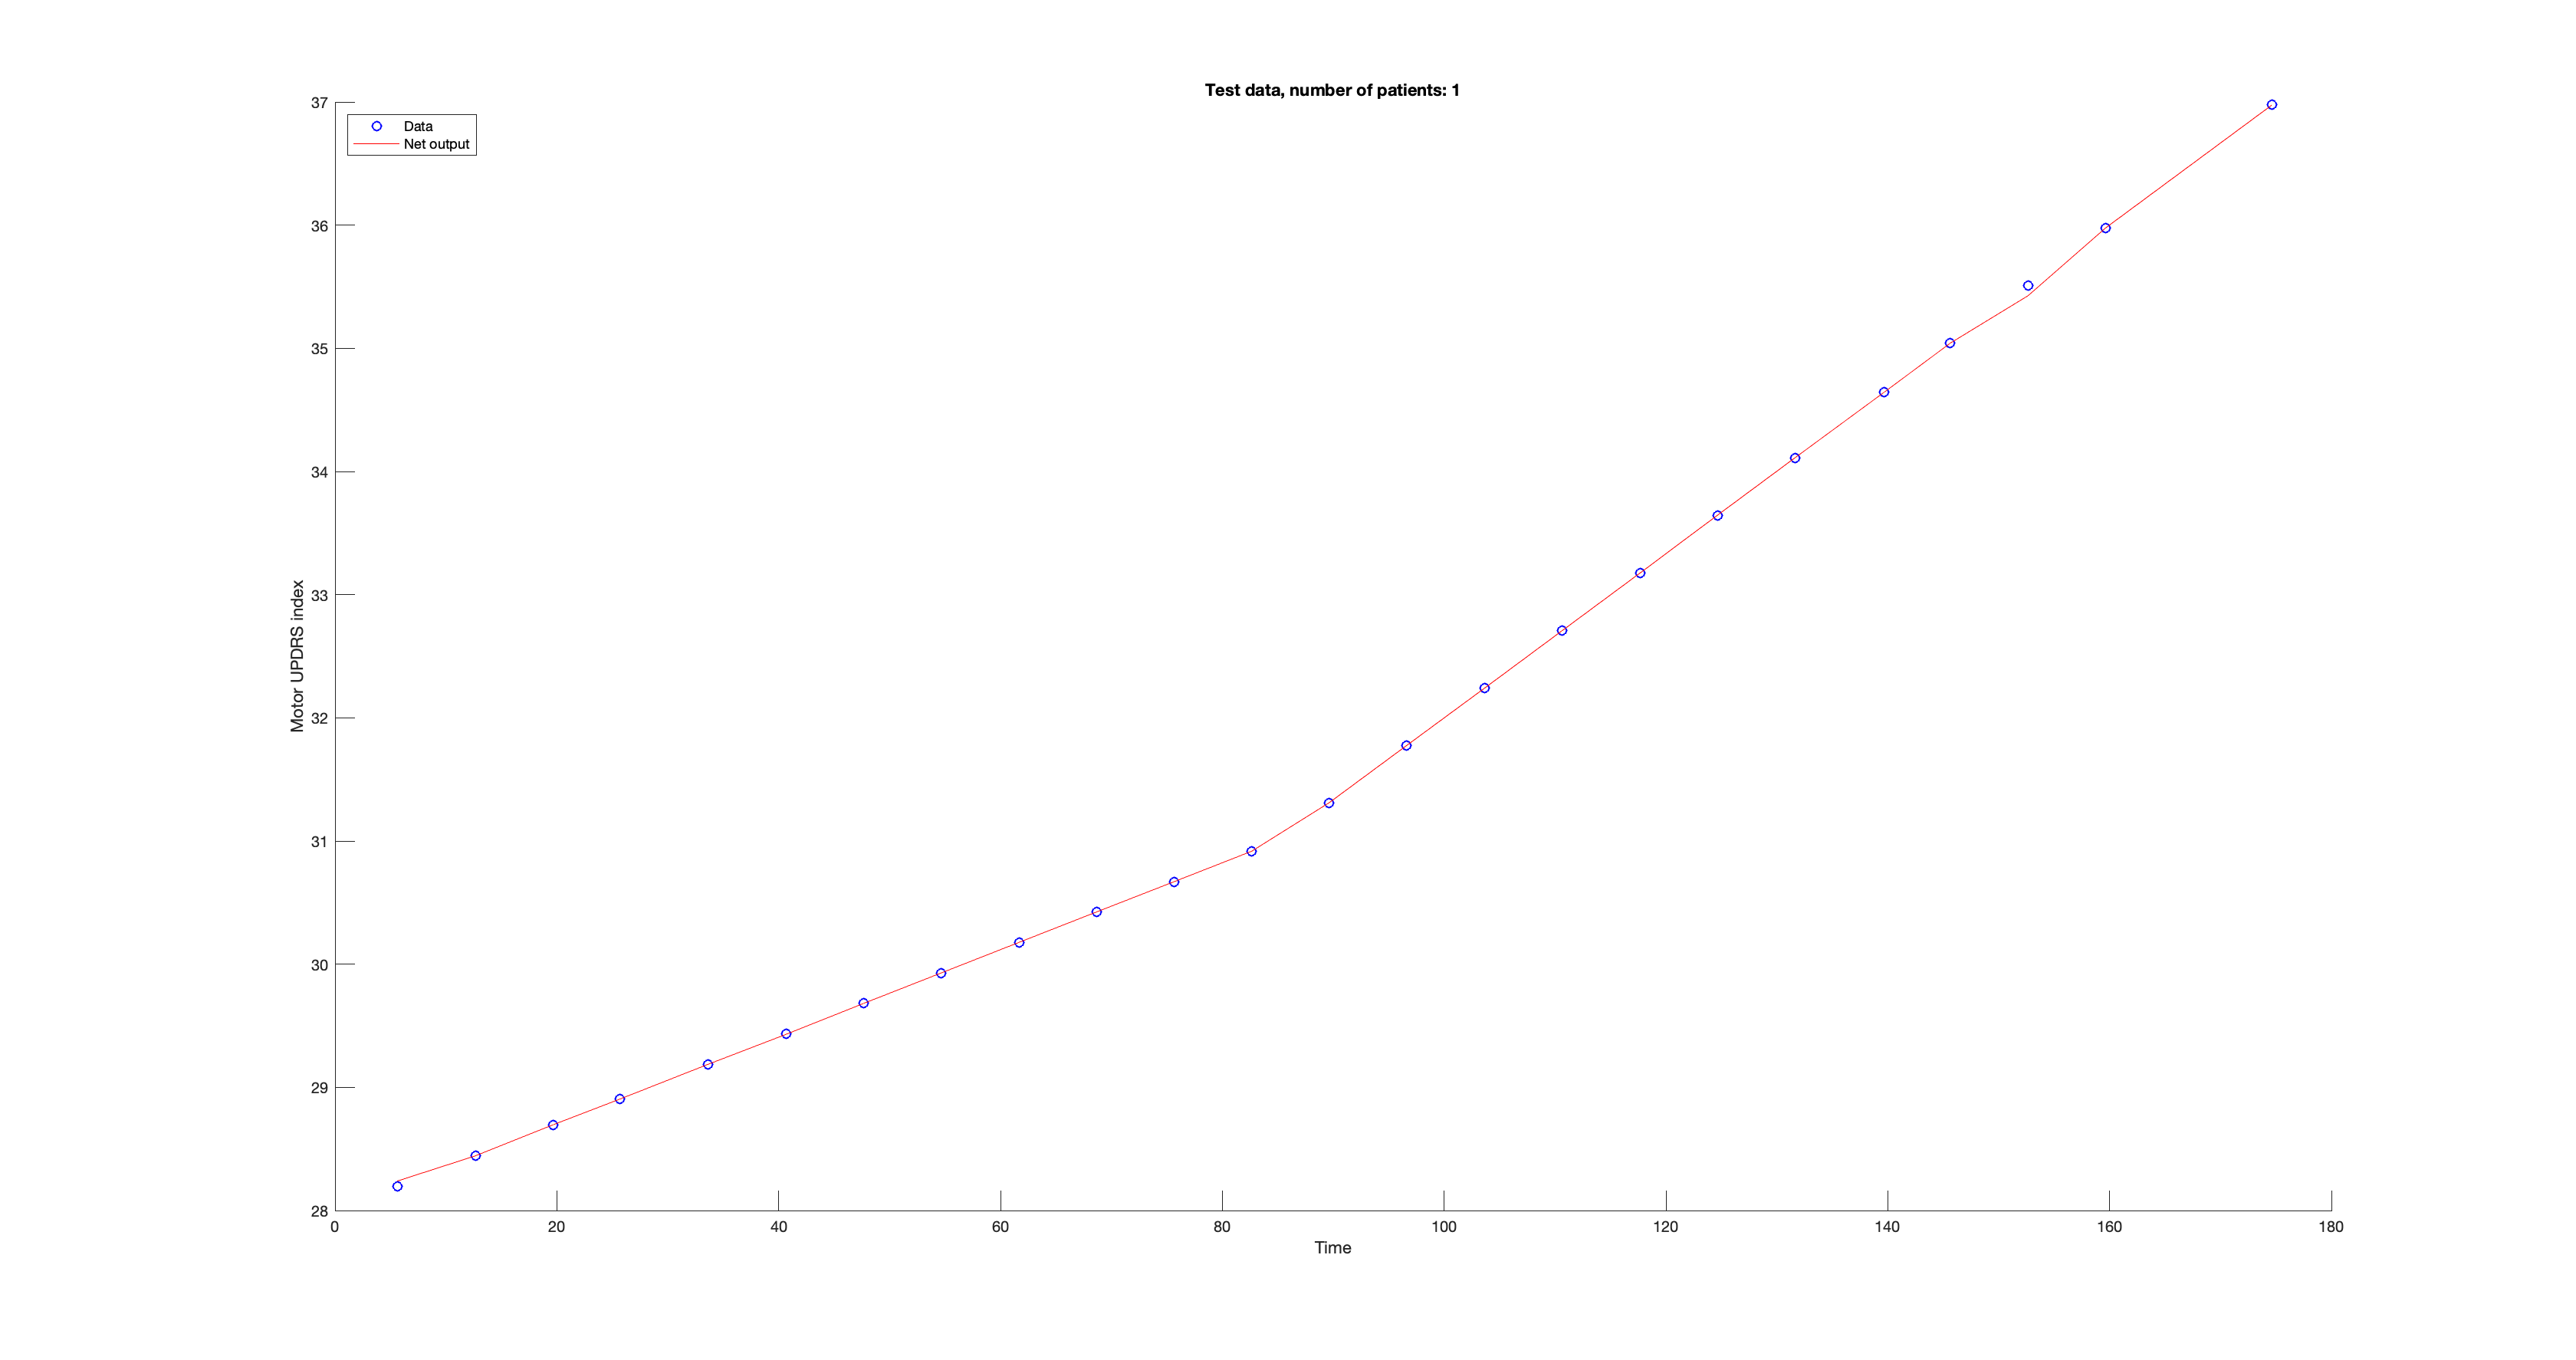
\includegraphics[width=1.05\textwidth]{test-normal-1.png}
\caption{Zbiór testowy, 1 pacjent}

\end{figure}

\begin{figure}[h!]

\centering
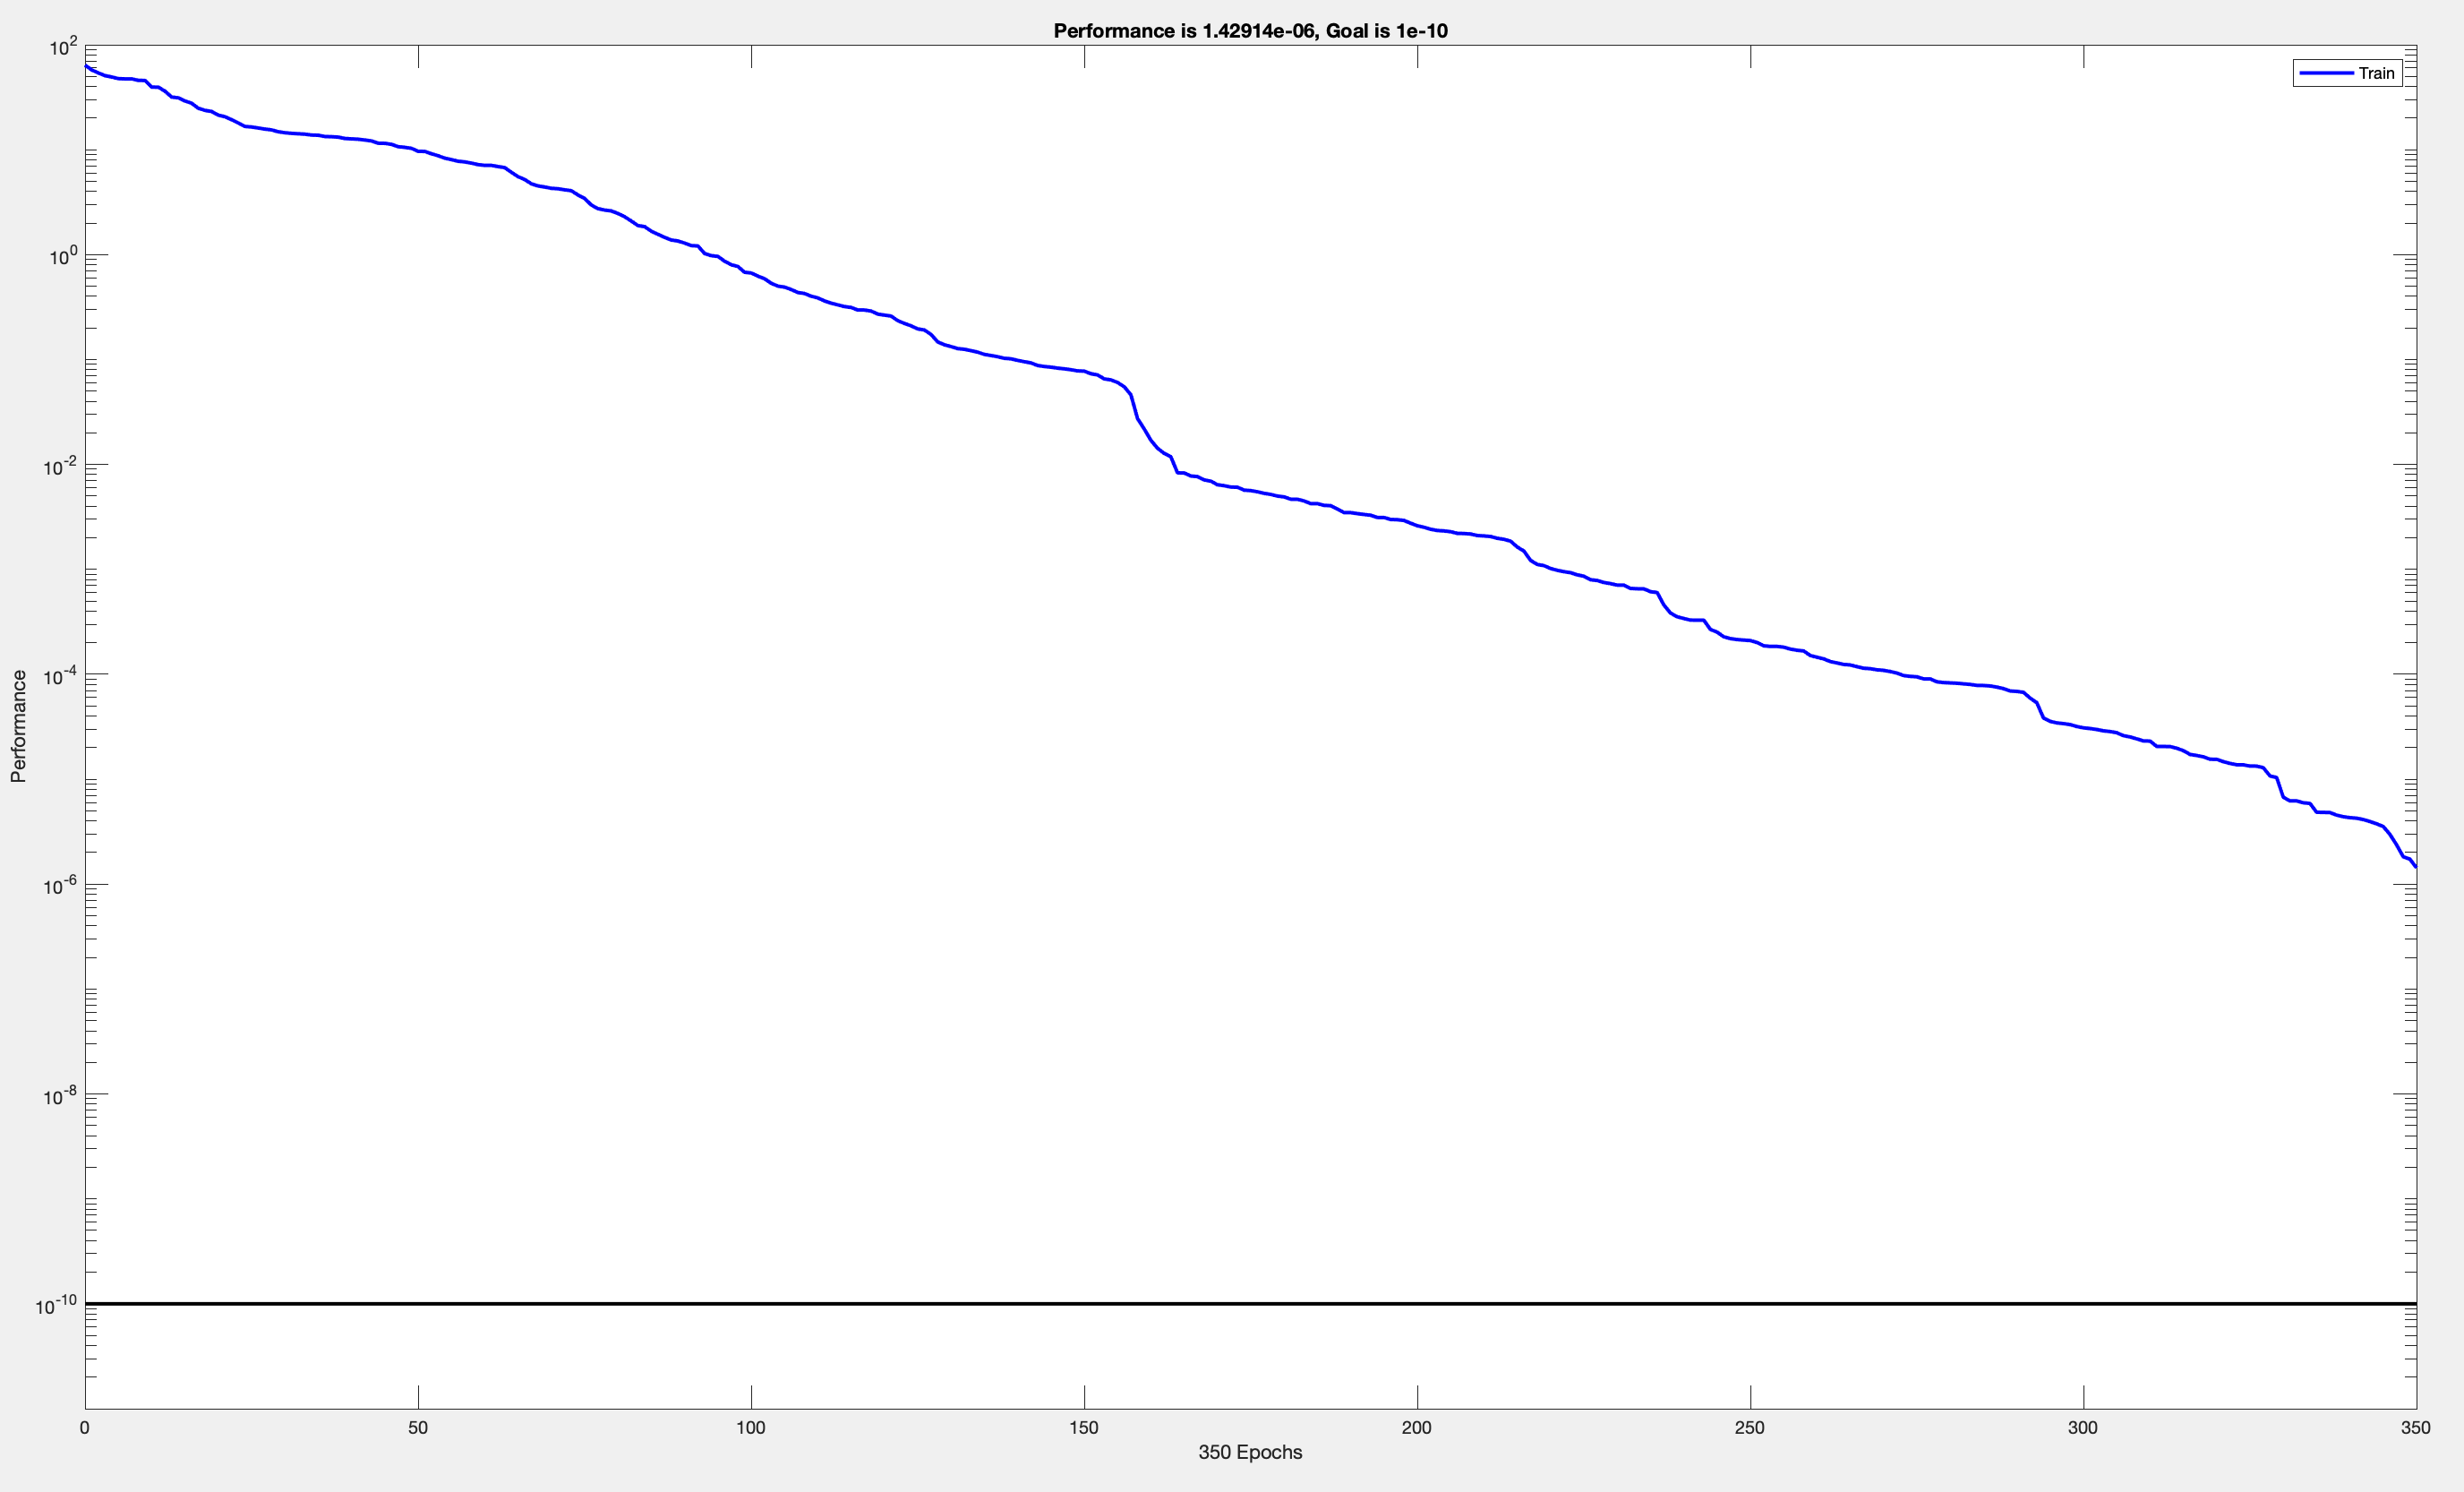
\includegraphics[width=0.9\textwidth]{mse-normal-3.png}
\caption{MSE dla 3 pacjentów}

\end{figure}

\begin{figure}[h!]

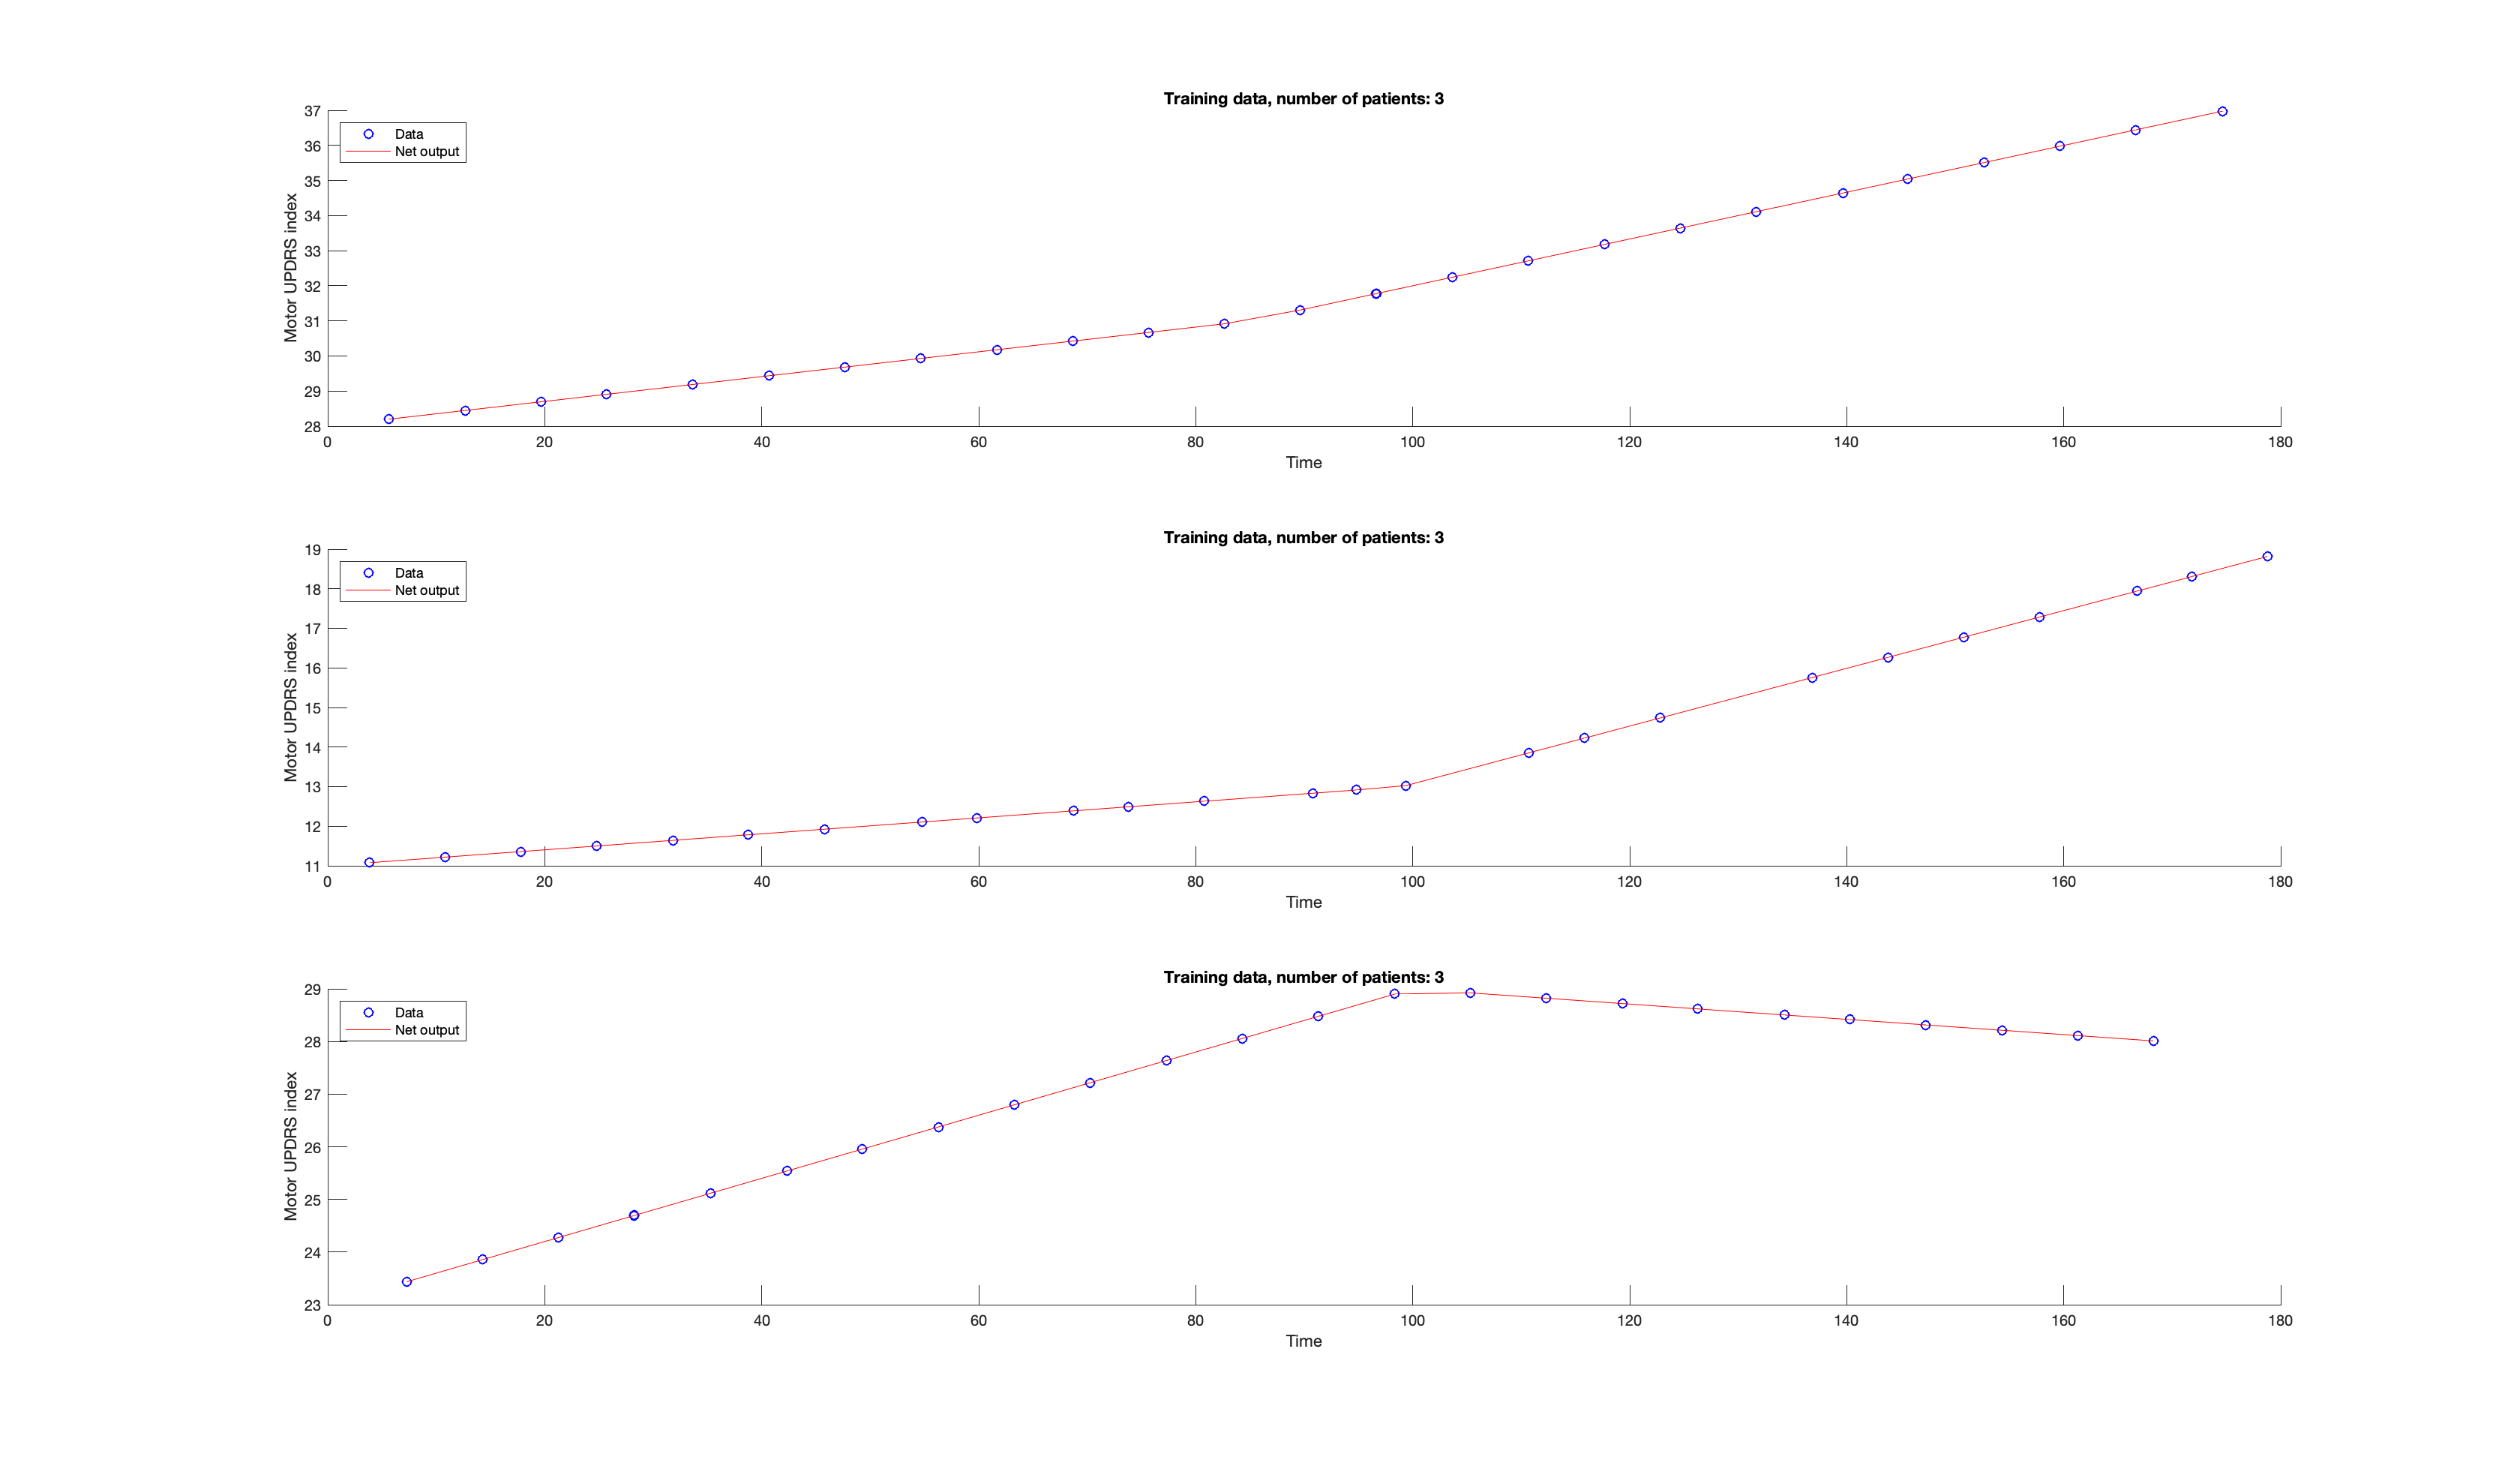
\includegraphics[width=1.05\textwidth]{training-normal-3.png}
\caption{Zbiór treningowy, 3 pacjentów}

\end{figure}

\begin{figure}[h!]

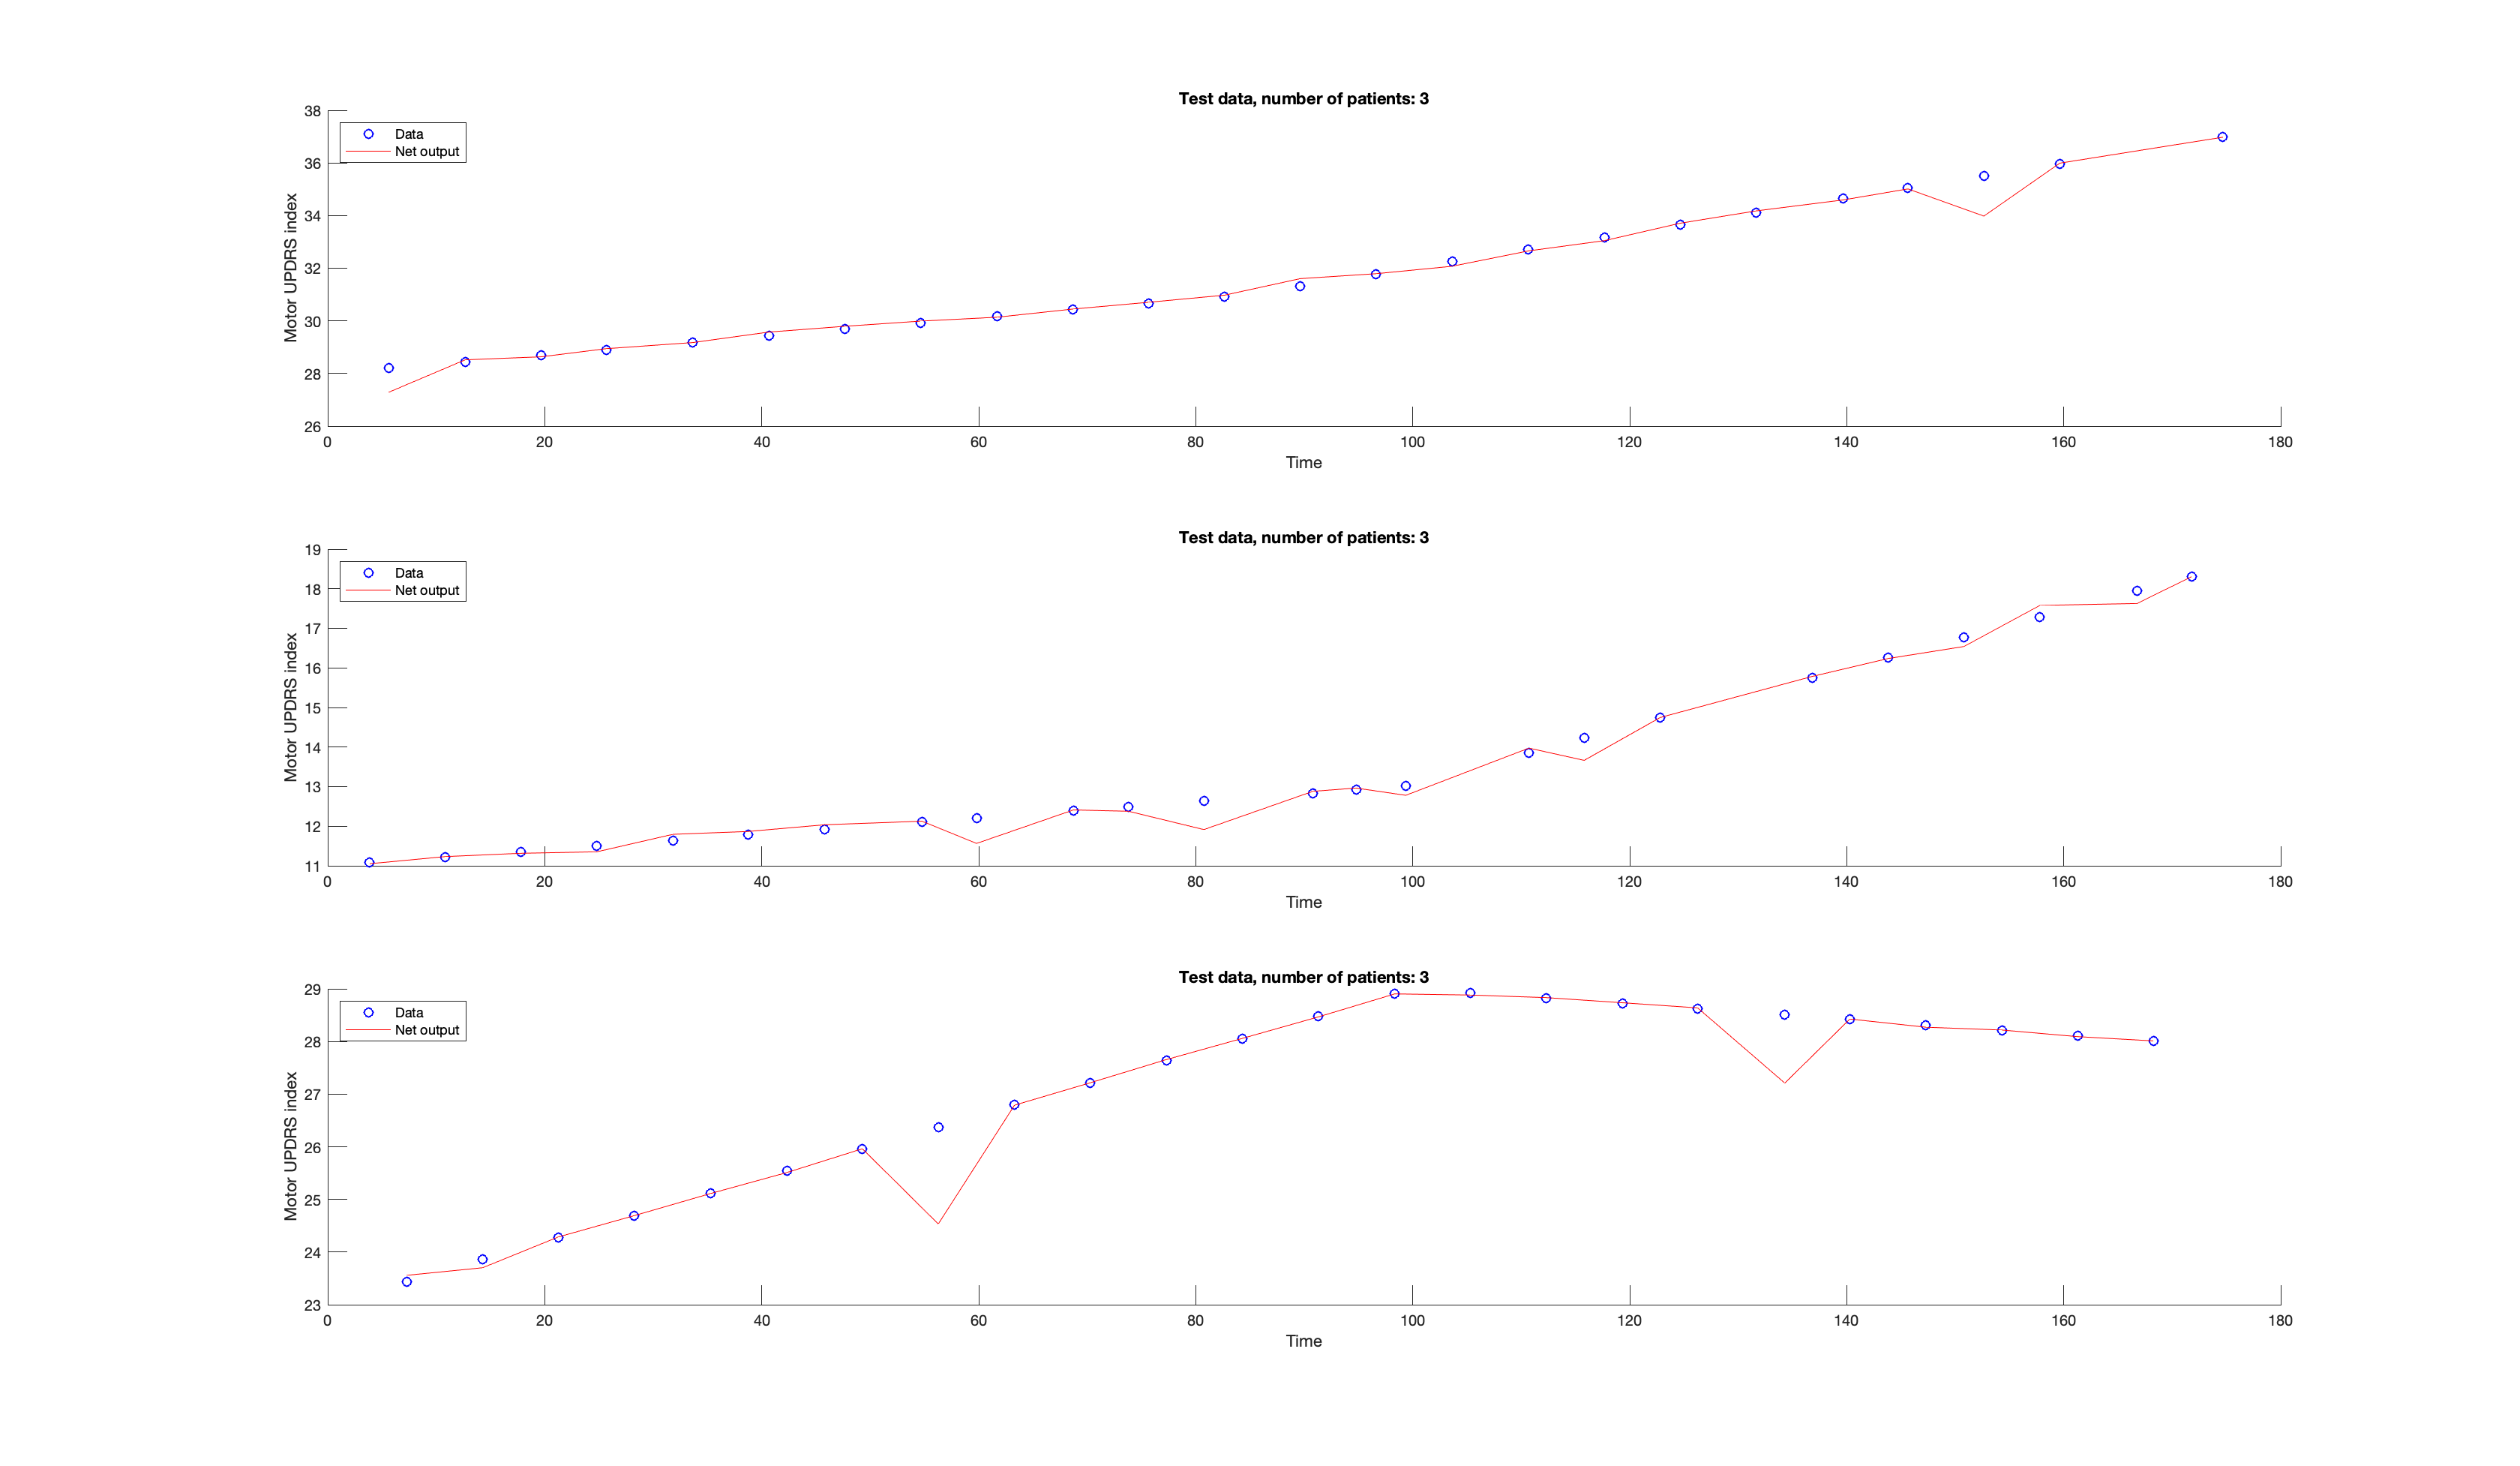
\includegraphics[width=1.0\textwidth]{test-normal-3.png}
\caption{Zbiór testowy, 3 pacjentów}

\end{figure}

\begin{figure}[h!]

\centering
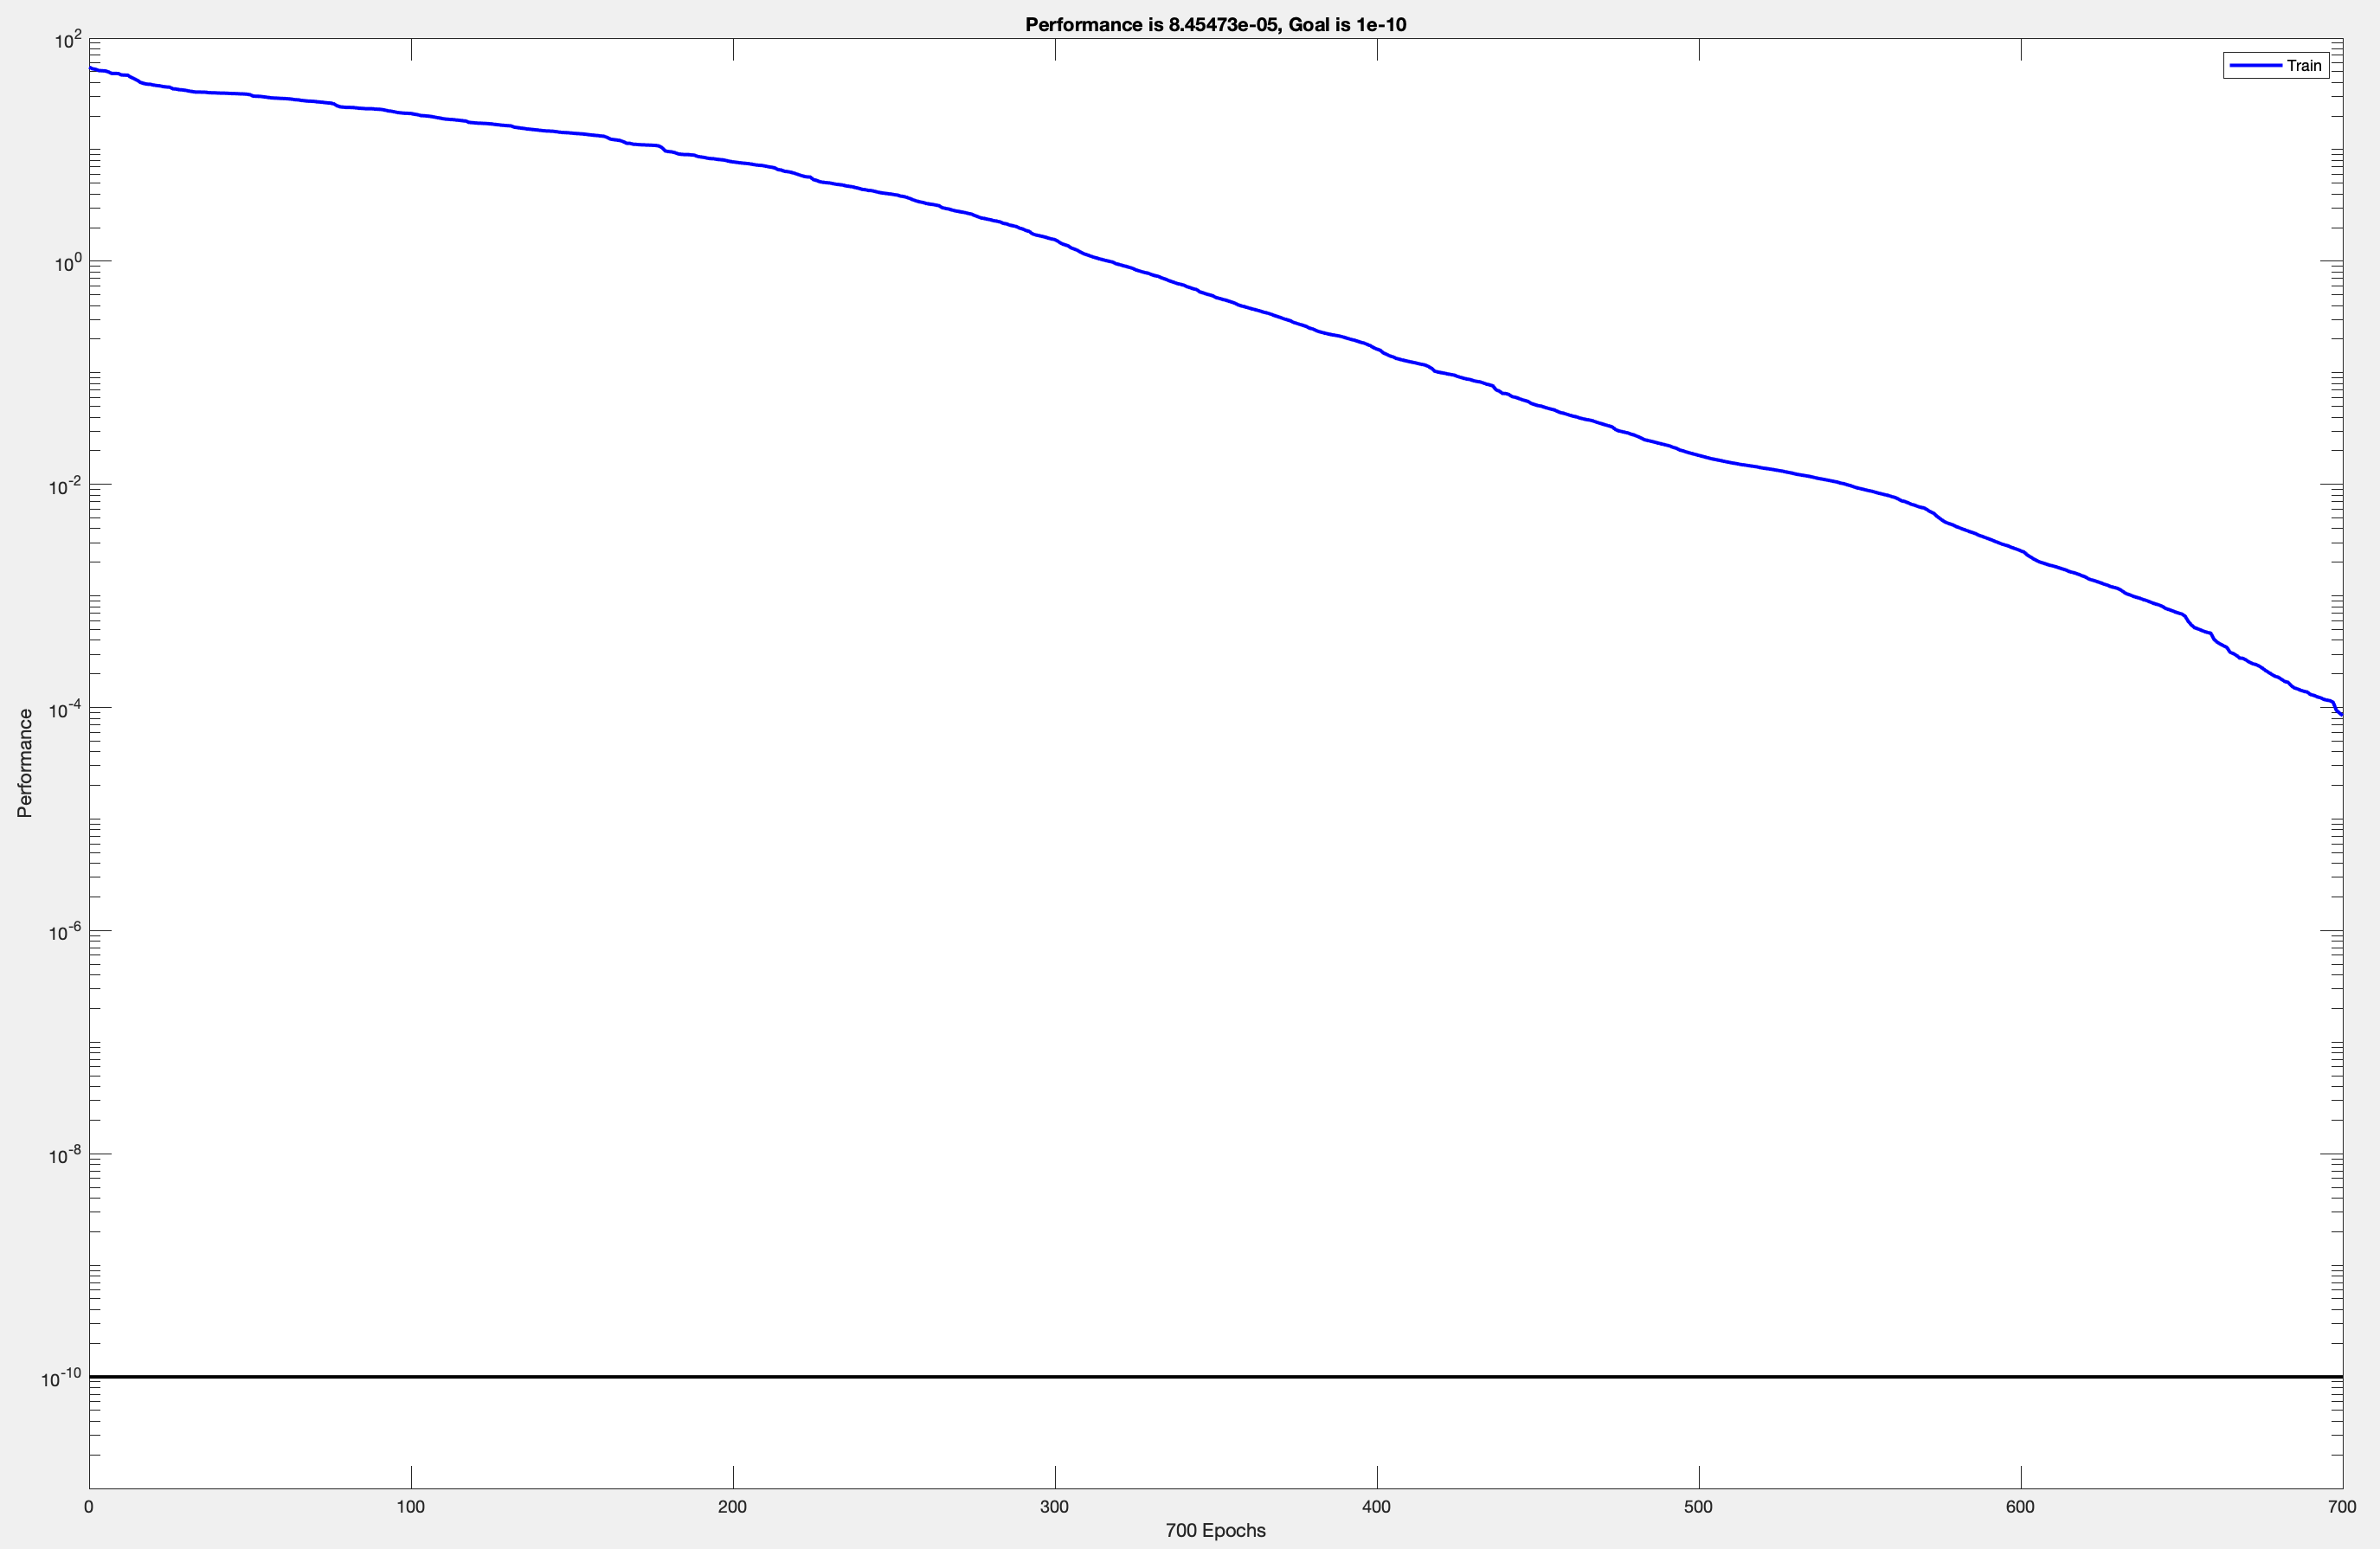
\includegraphics[width=0.9\textwidth]{mse-normal-6.png}
\caption{MSE dla 6 pacjentów}

\end{figure}

\begin{figure}[h!]

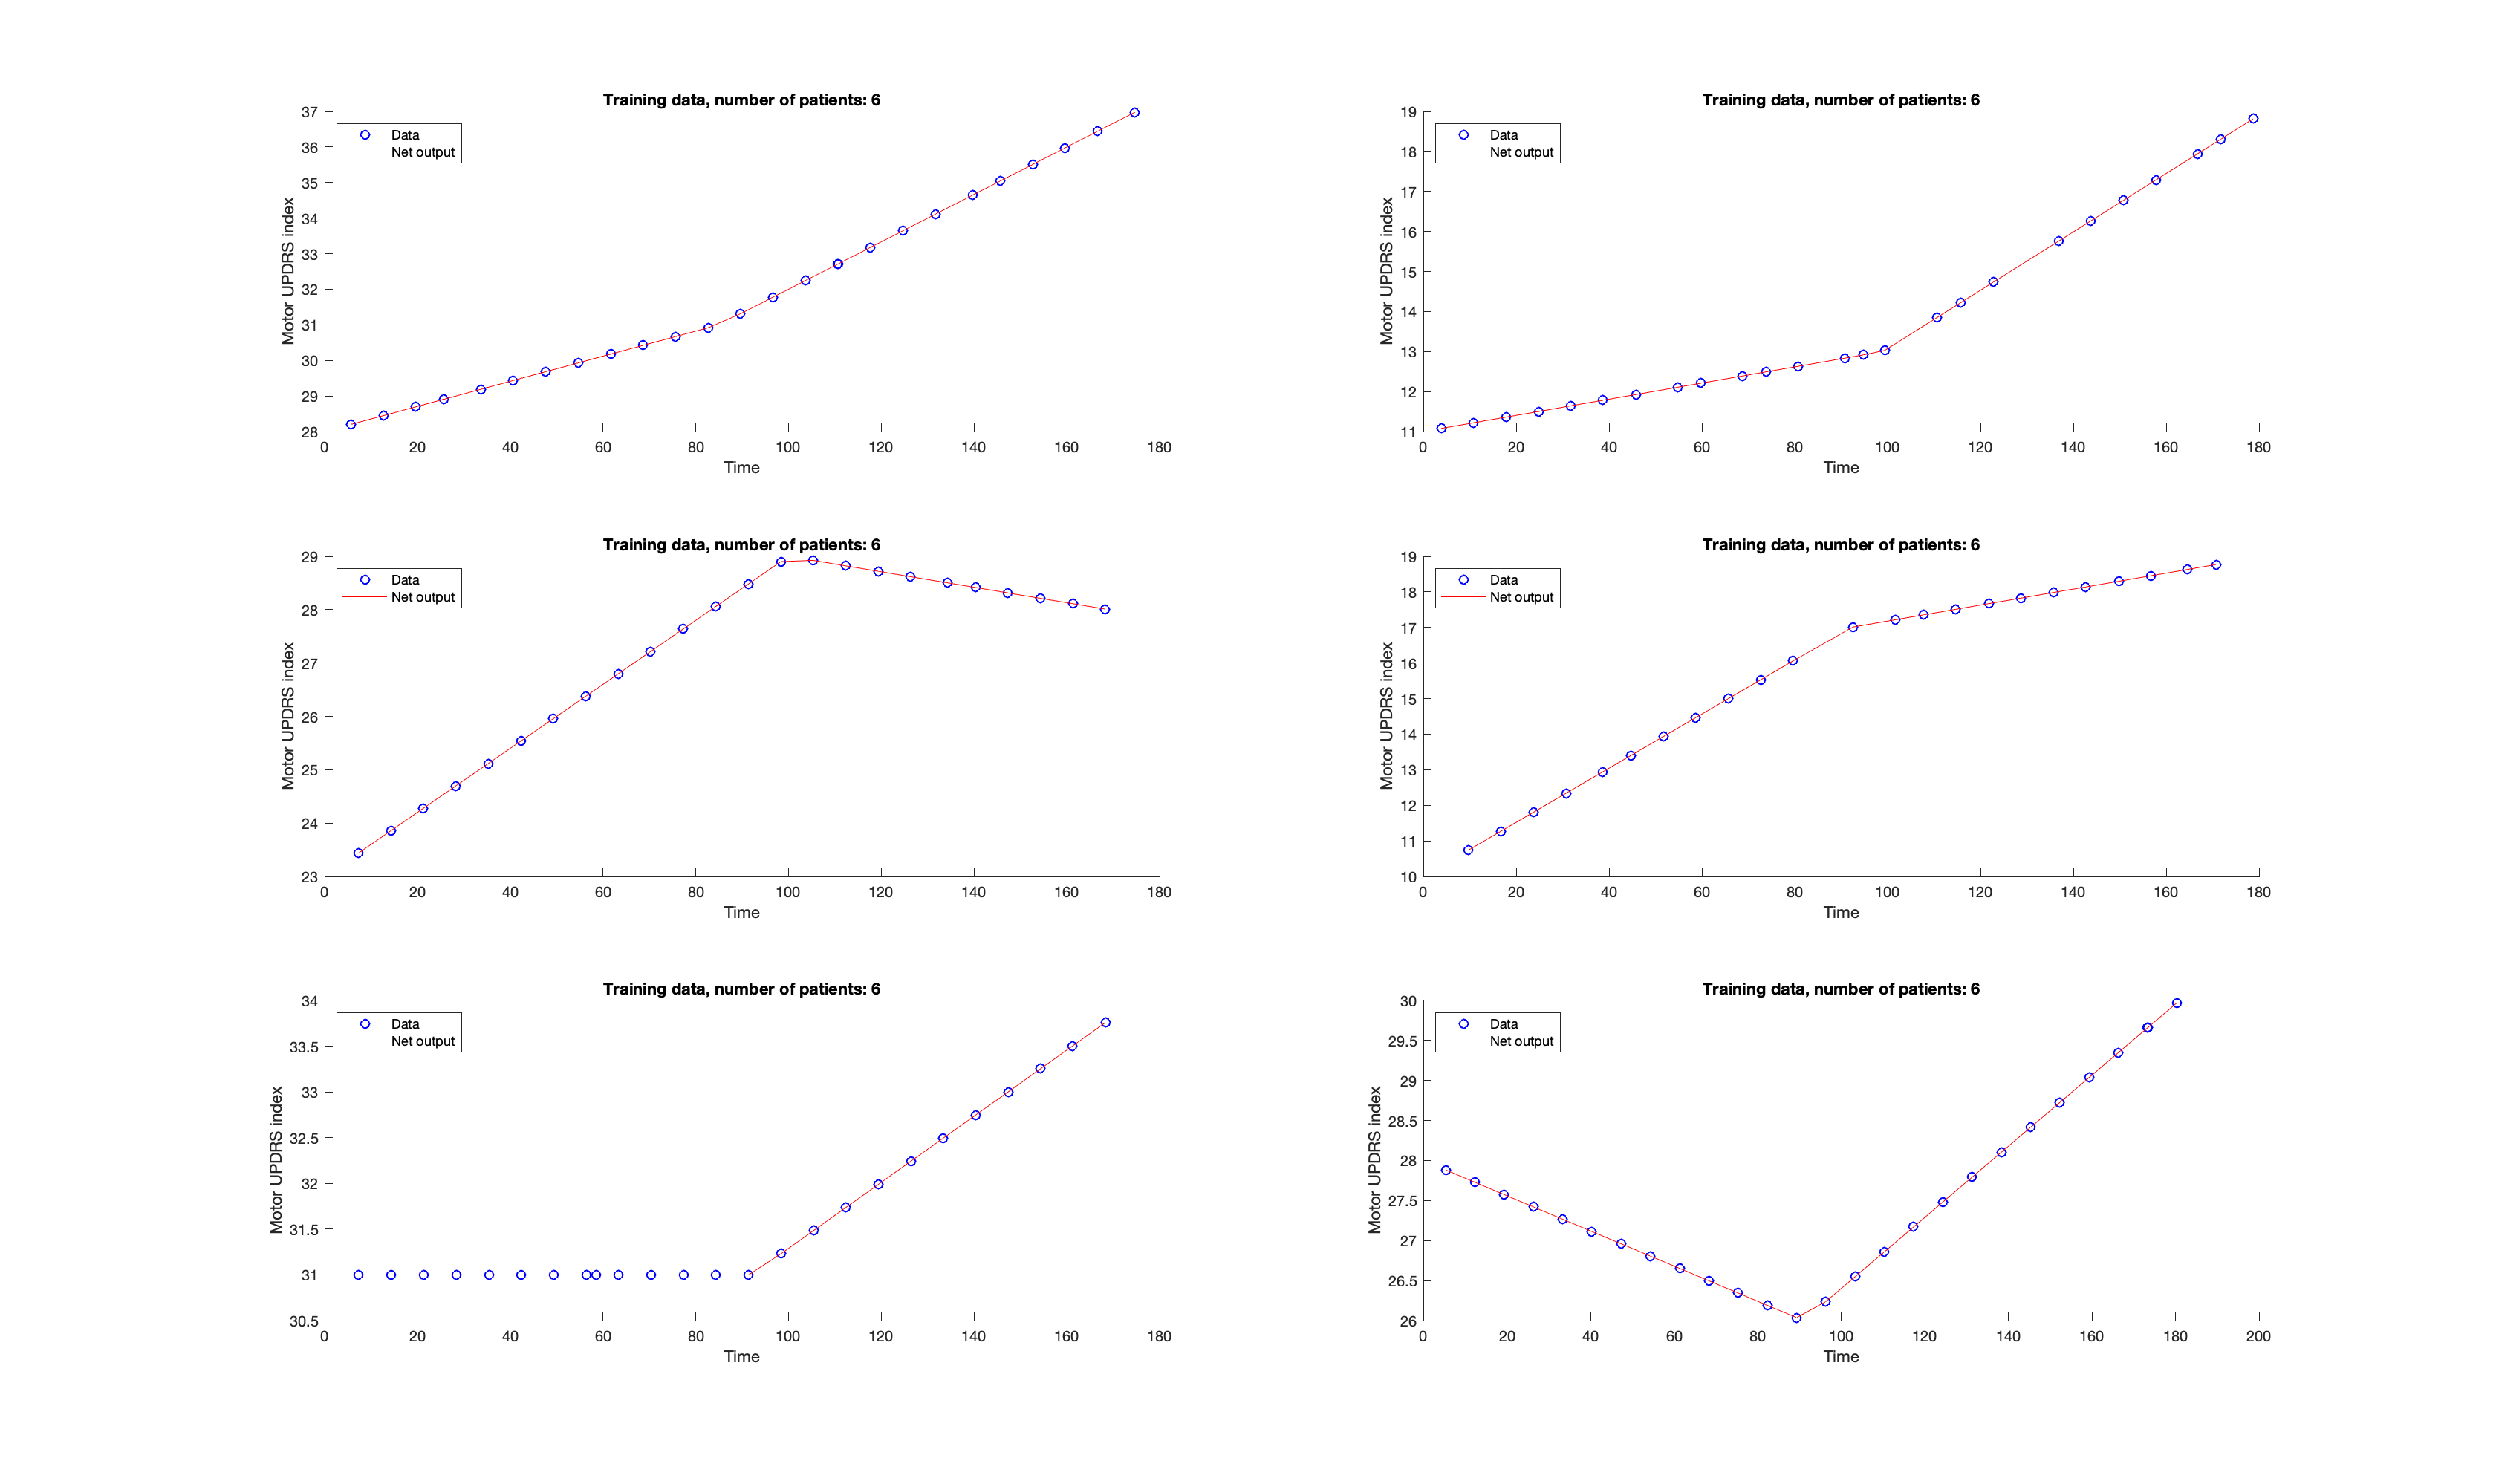
\includegraphics[width=1.0\textwidth]{training-normal-6.png}
\caption{Zbiór treningowy, 6 pacjentów}

\end{figure}

\begin{figure}[h!]

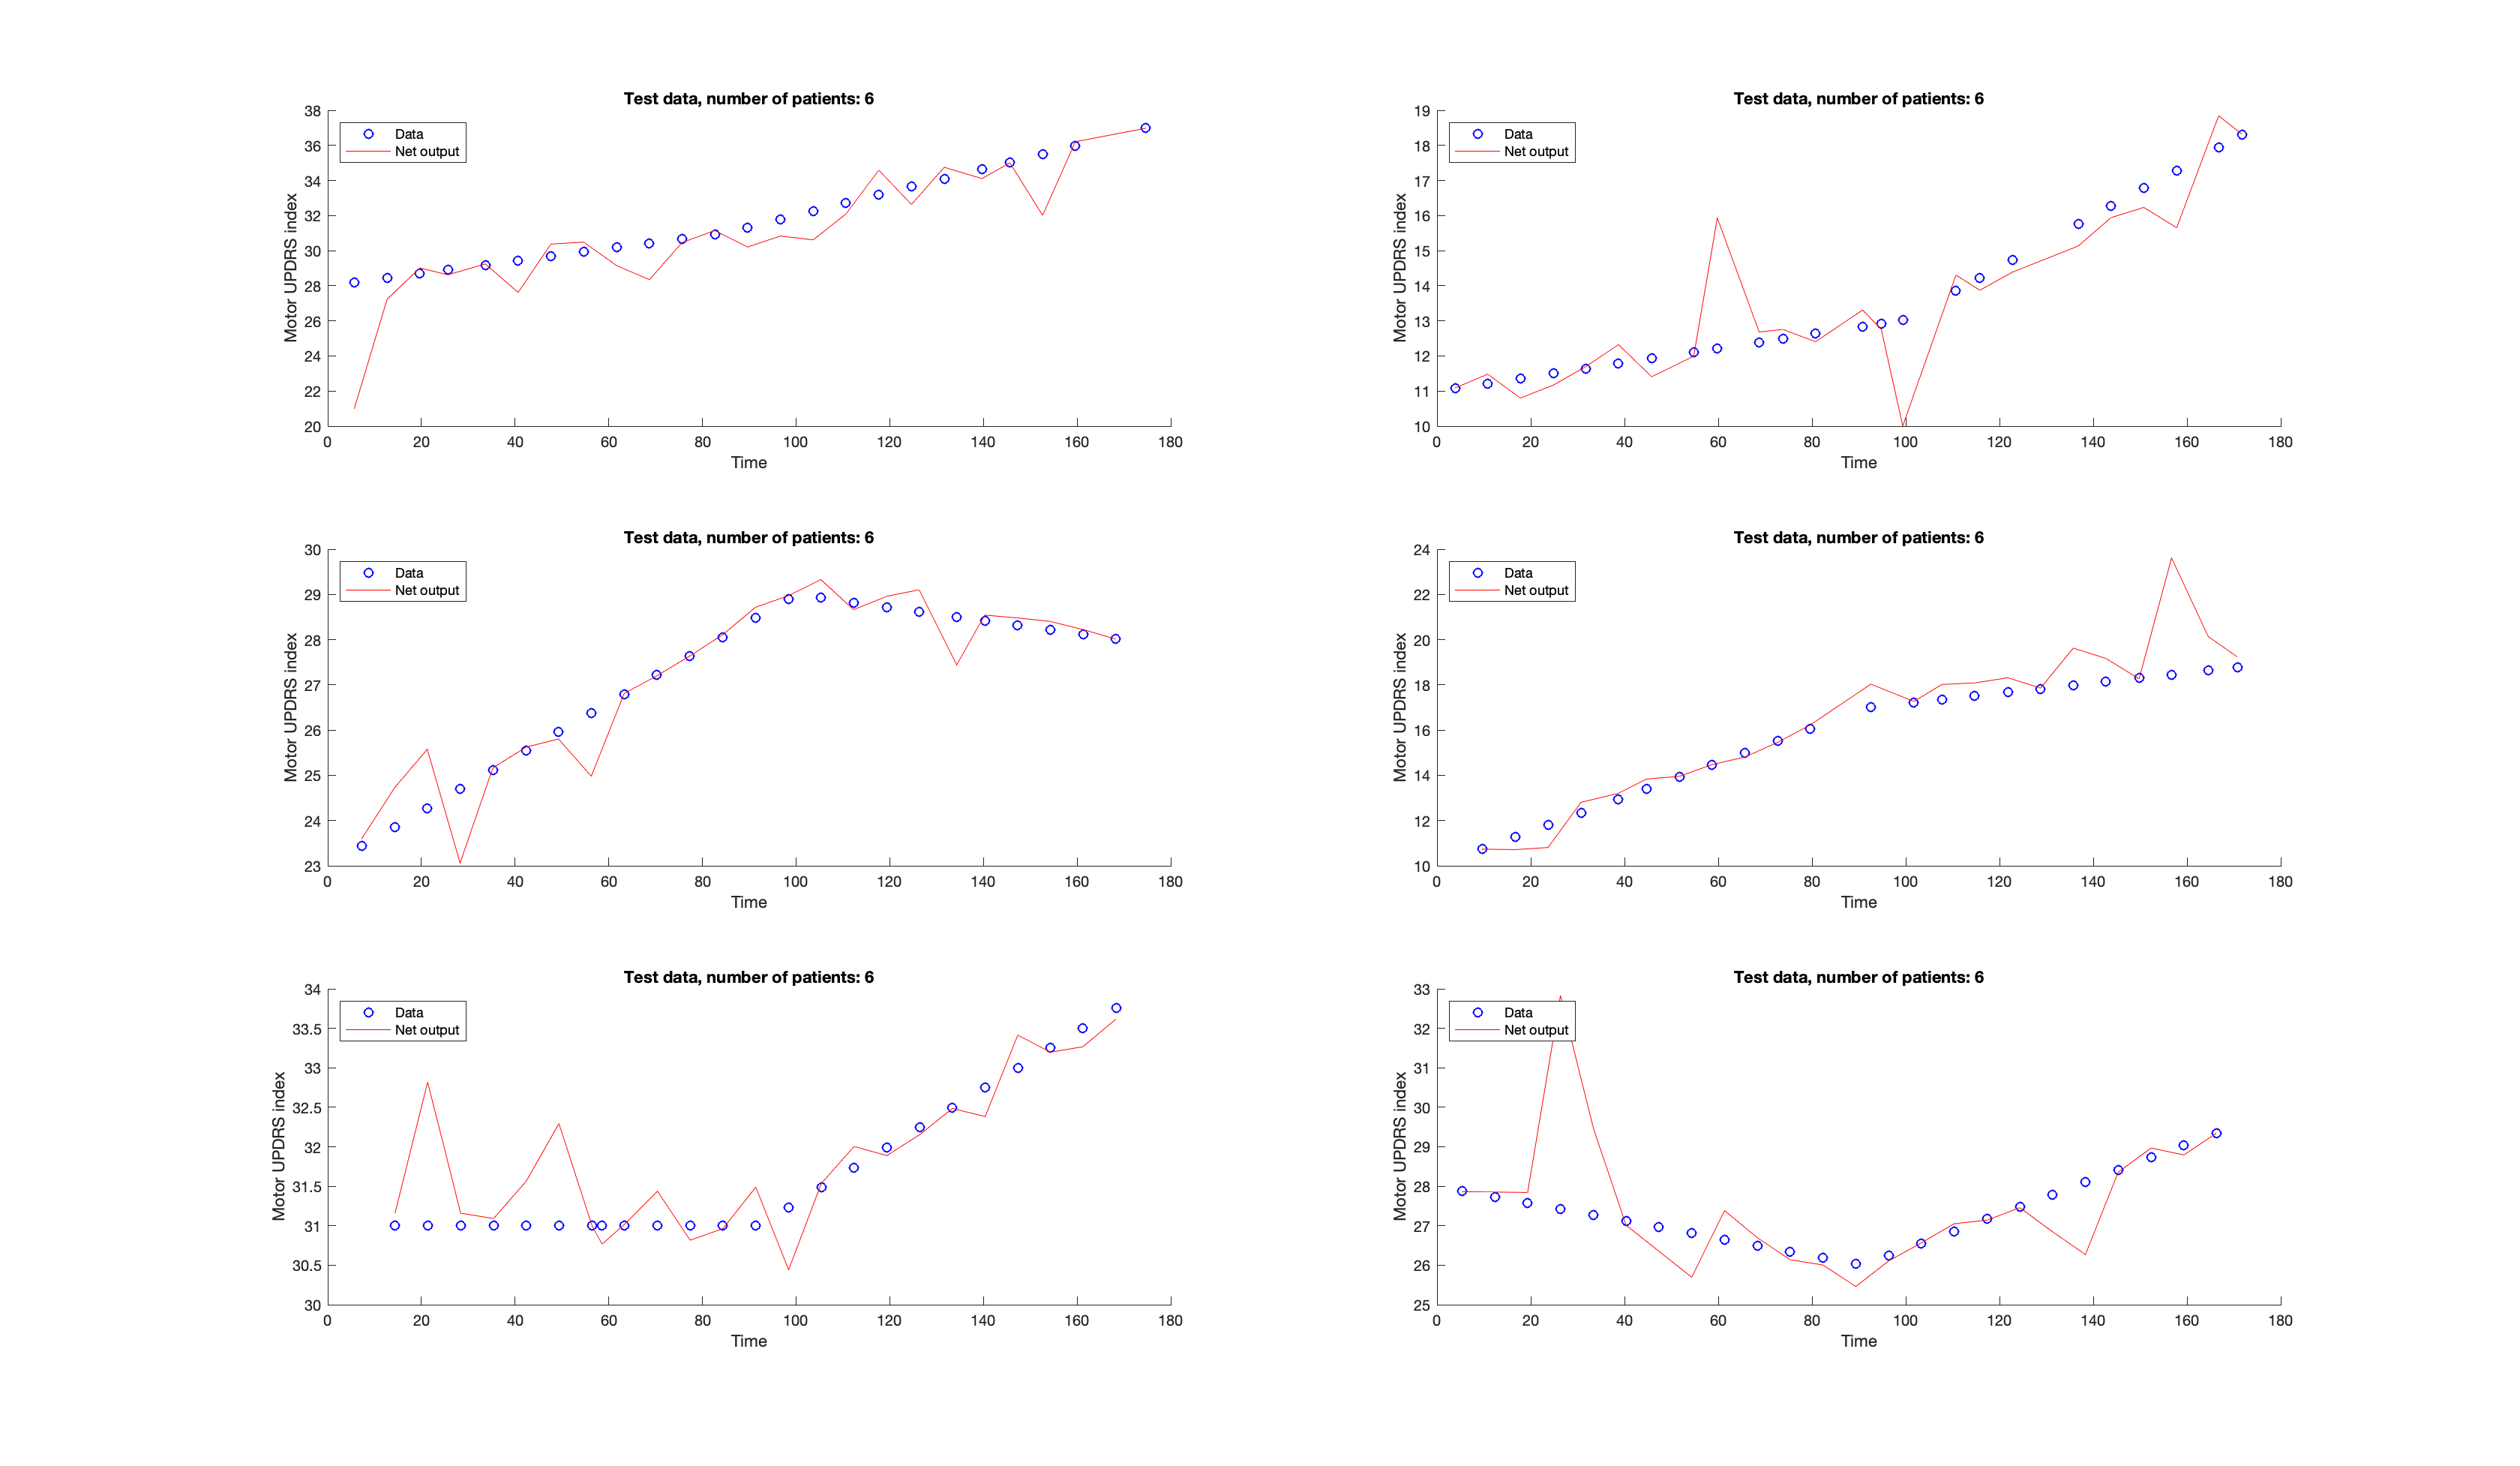
\includegraphics[width=1.0\textwidth]{test-normal-6.png}
\caption{Zbiór testowy, 6 pacjentów}

\end{figure}

\newpage

Na powyższych wykresach można zaobserwować, że dla małej ilości pacjentów i dużej ilości danych uczących sieć nie wykazuje problemów z uczeniem. Skuteczność predykcji w przypadku danych testowych jest na wysokim poziomie.

\subsection{Dane z duplikatami próbek czasowych z dużą ilością pacjentów}

Parametry uczenia:
\begin{itemize}
\item Mean squared error: $10^{-9}$
\item Spread constant: $10$
\end{itemize}

\begin{figure}[h!]

\centering
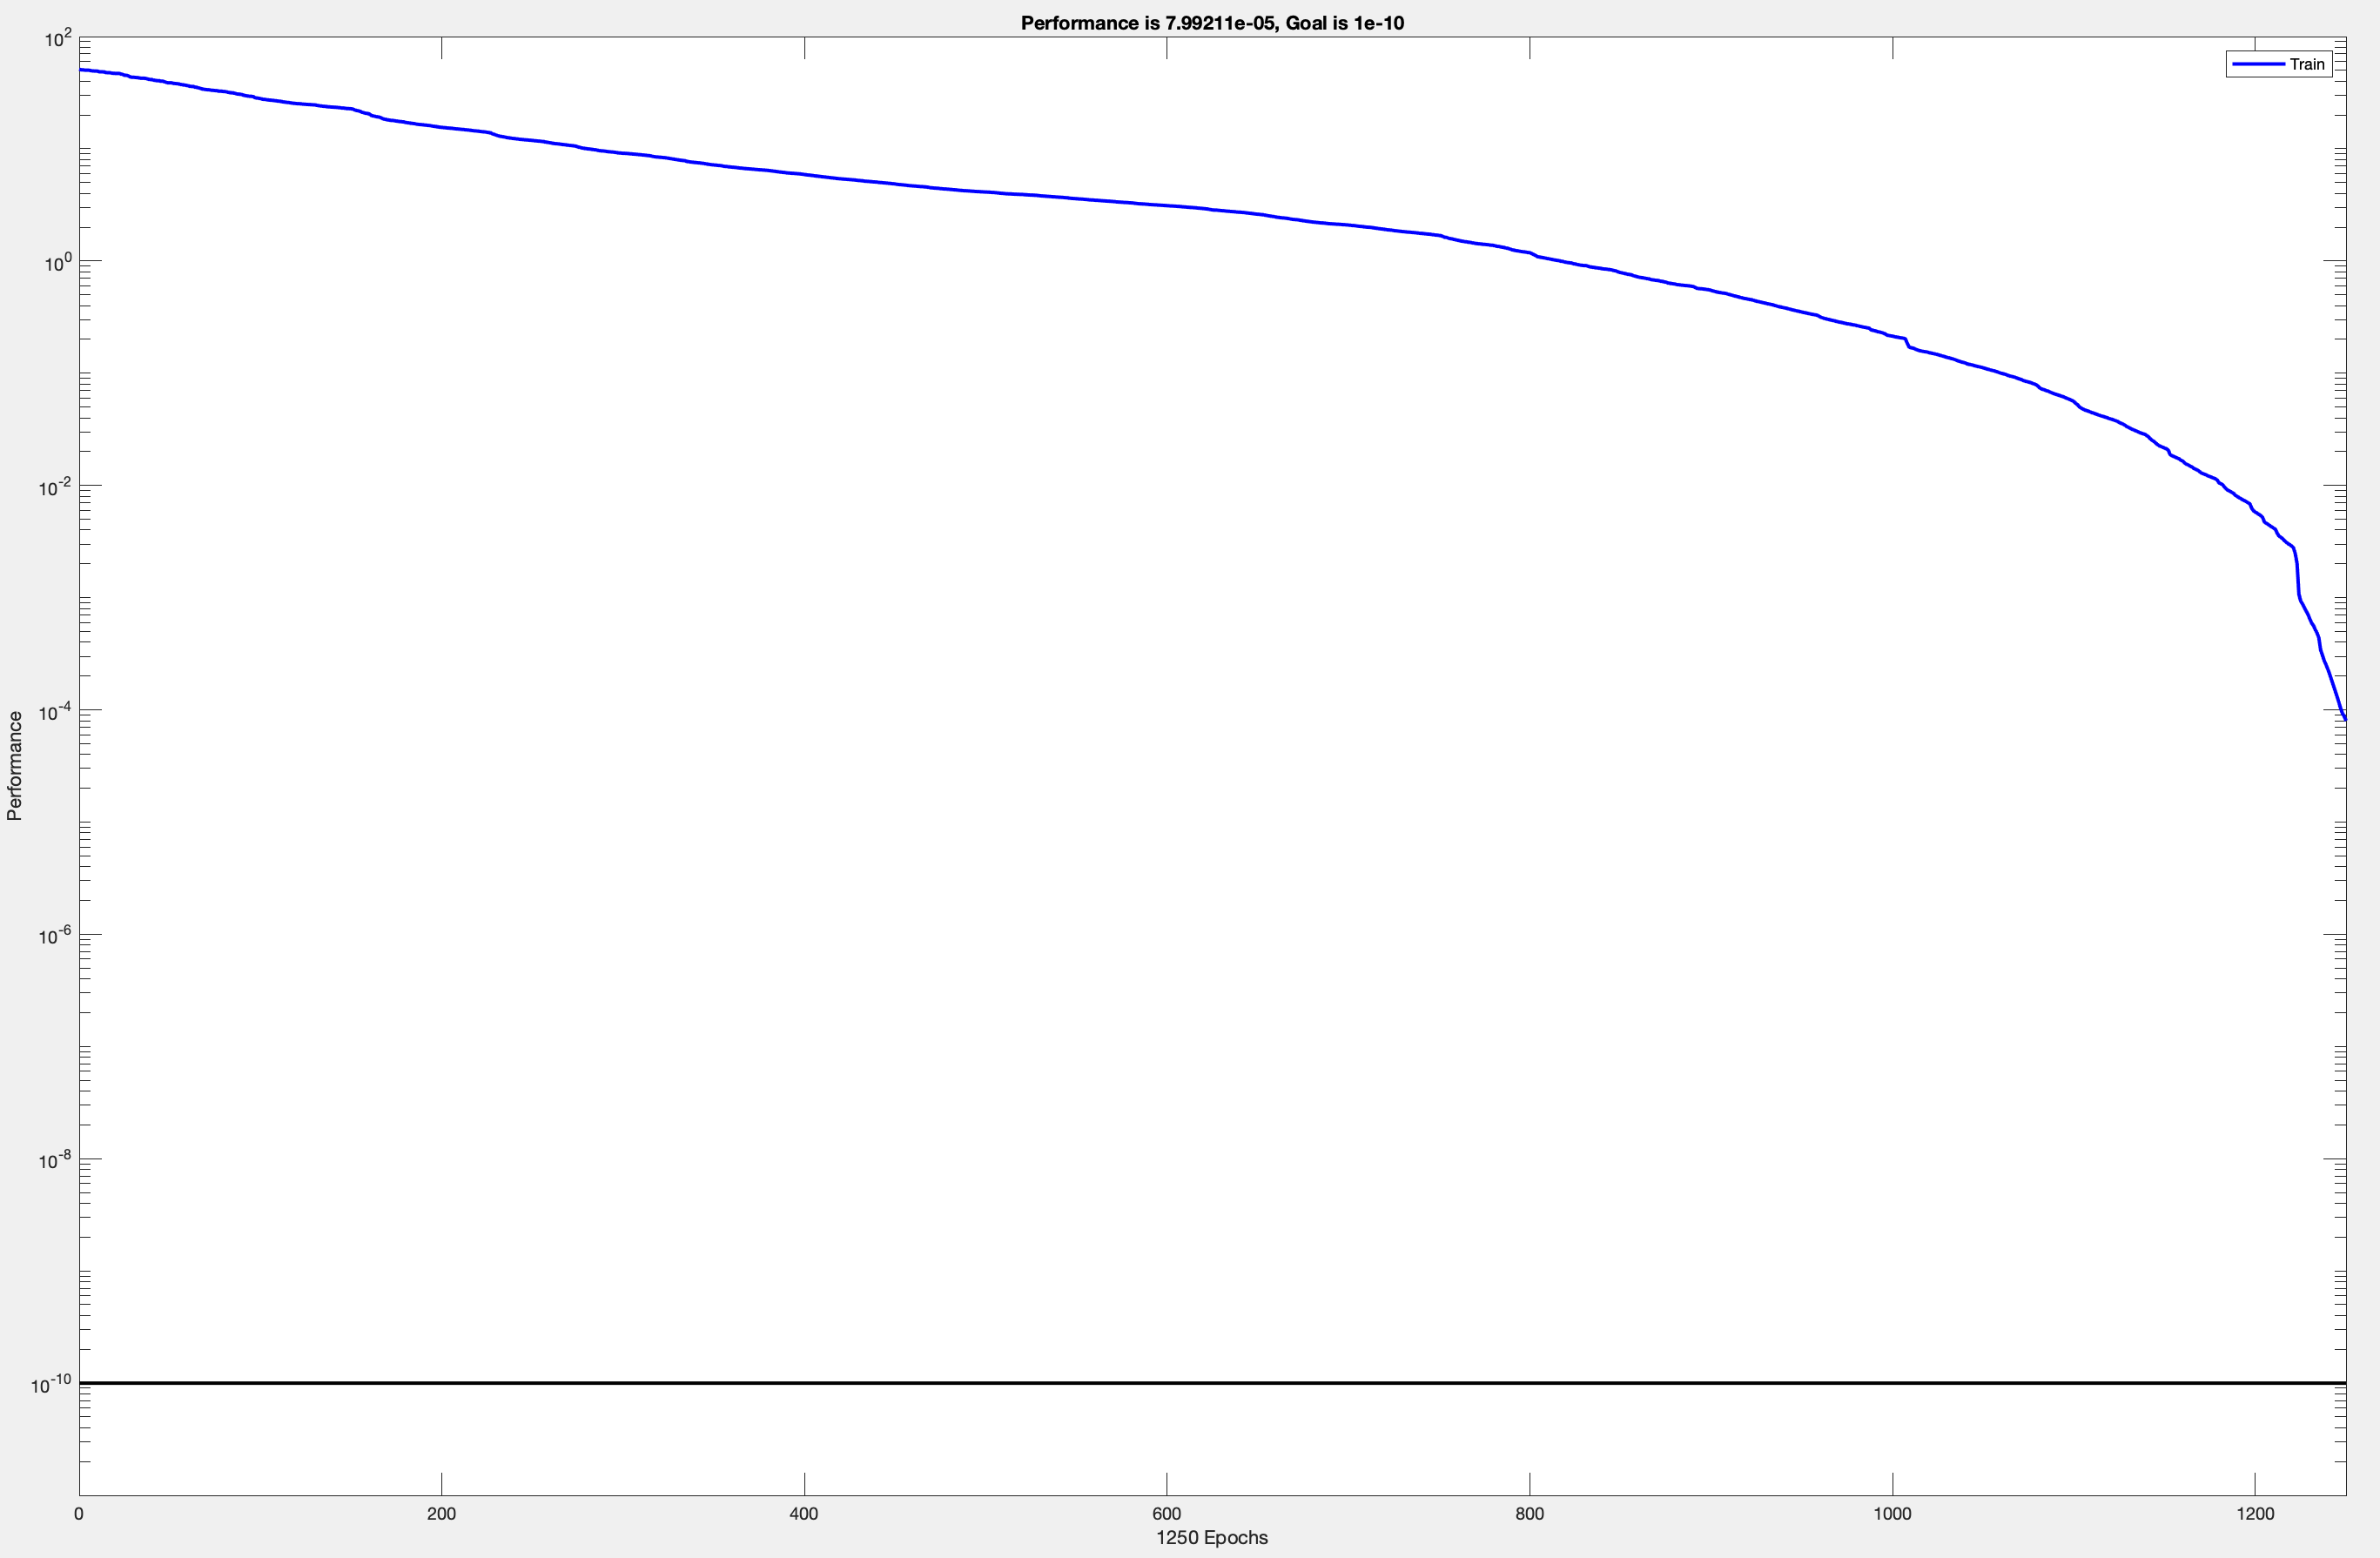
\includegraphics[width=0.9\textwidth]{mse-normal-10.png}
\caption{MSE dla 10 pacjentów}

\end{figure}

\begin{figure}[h!]

\centering
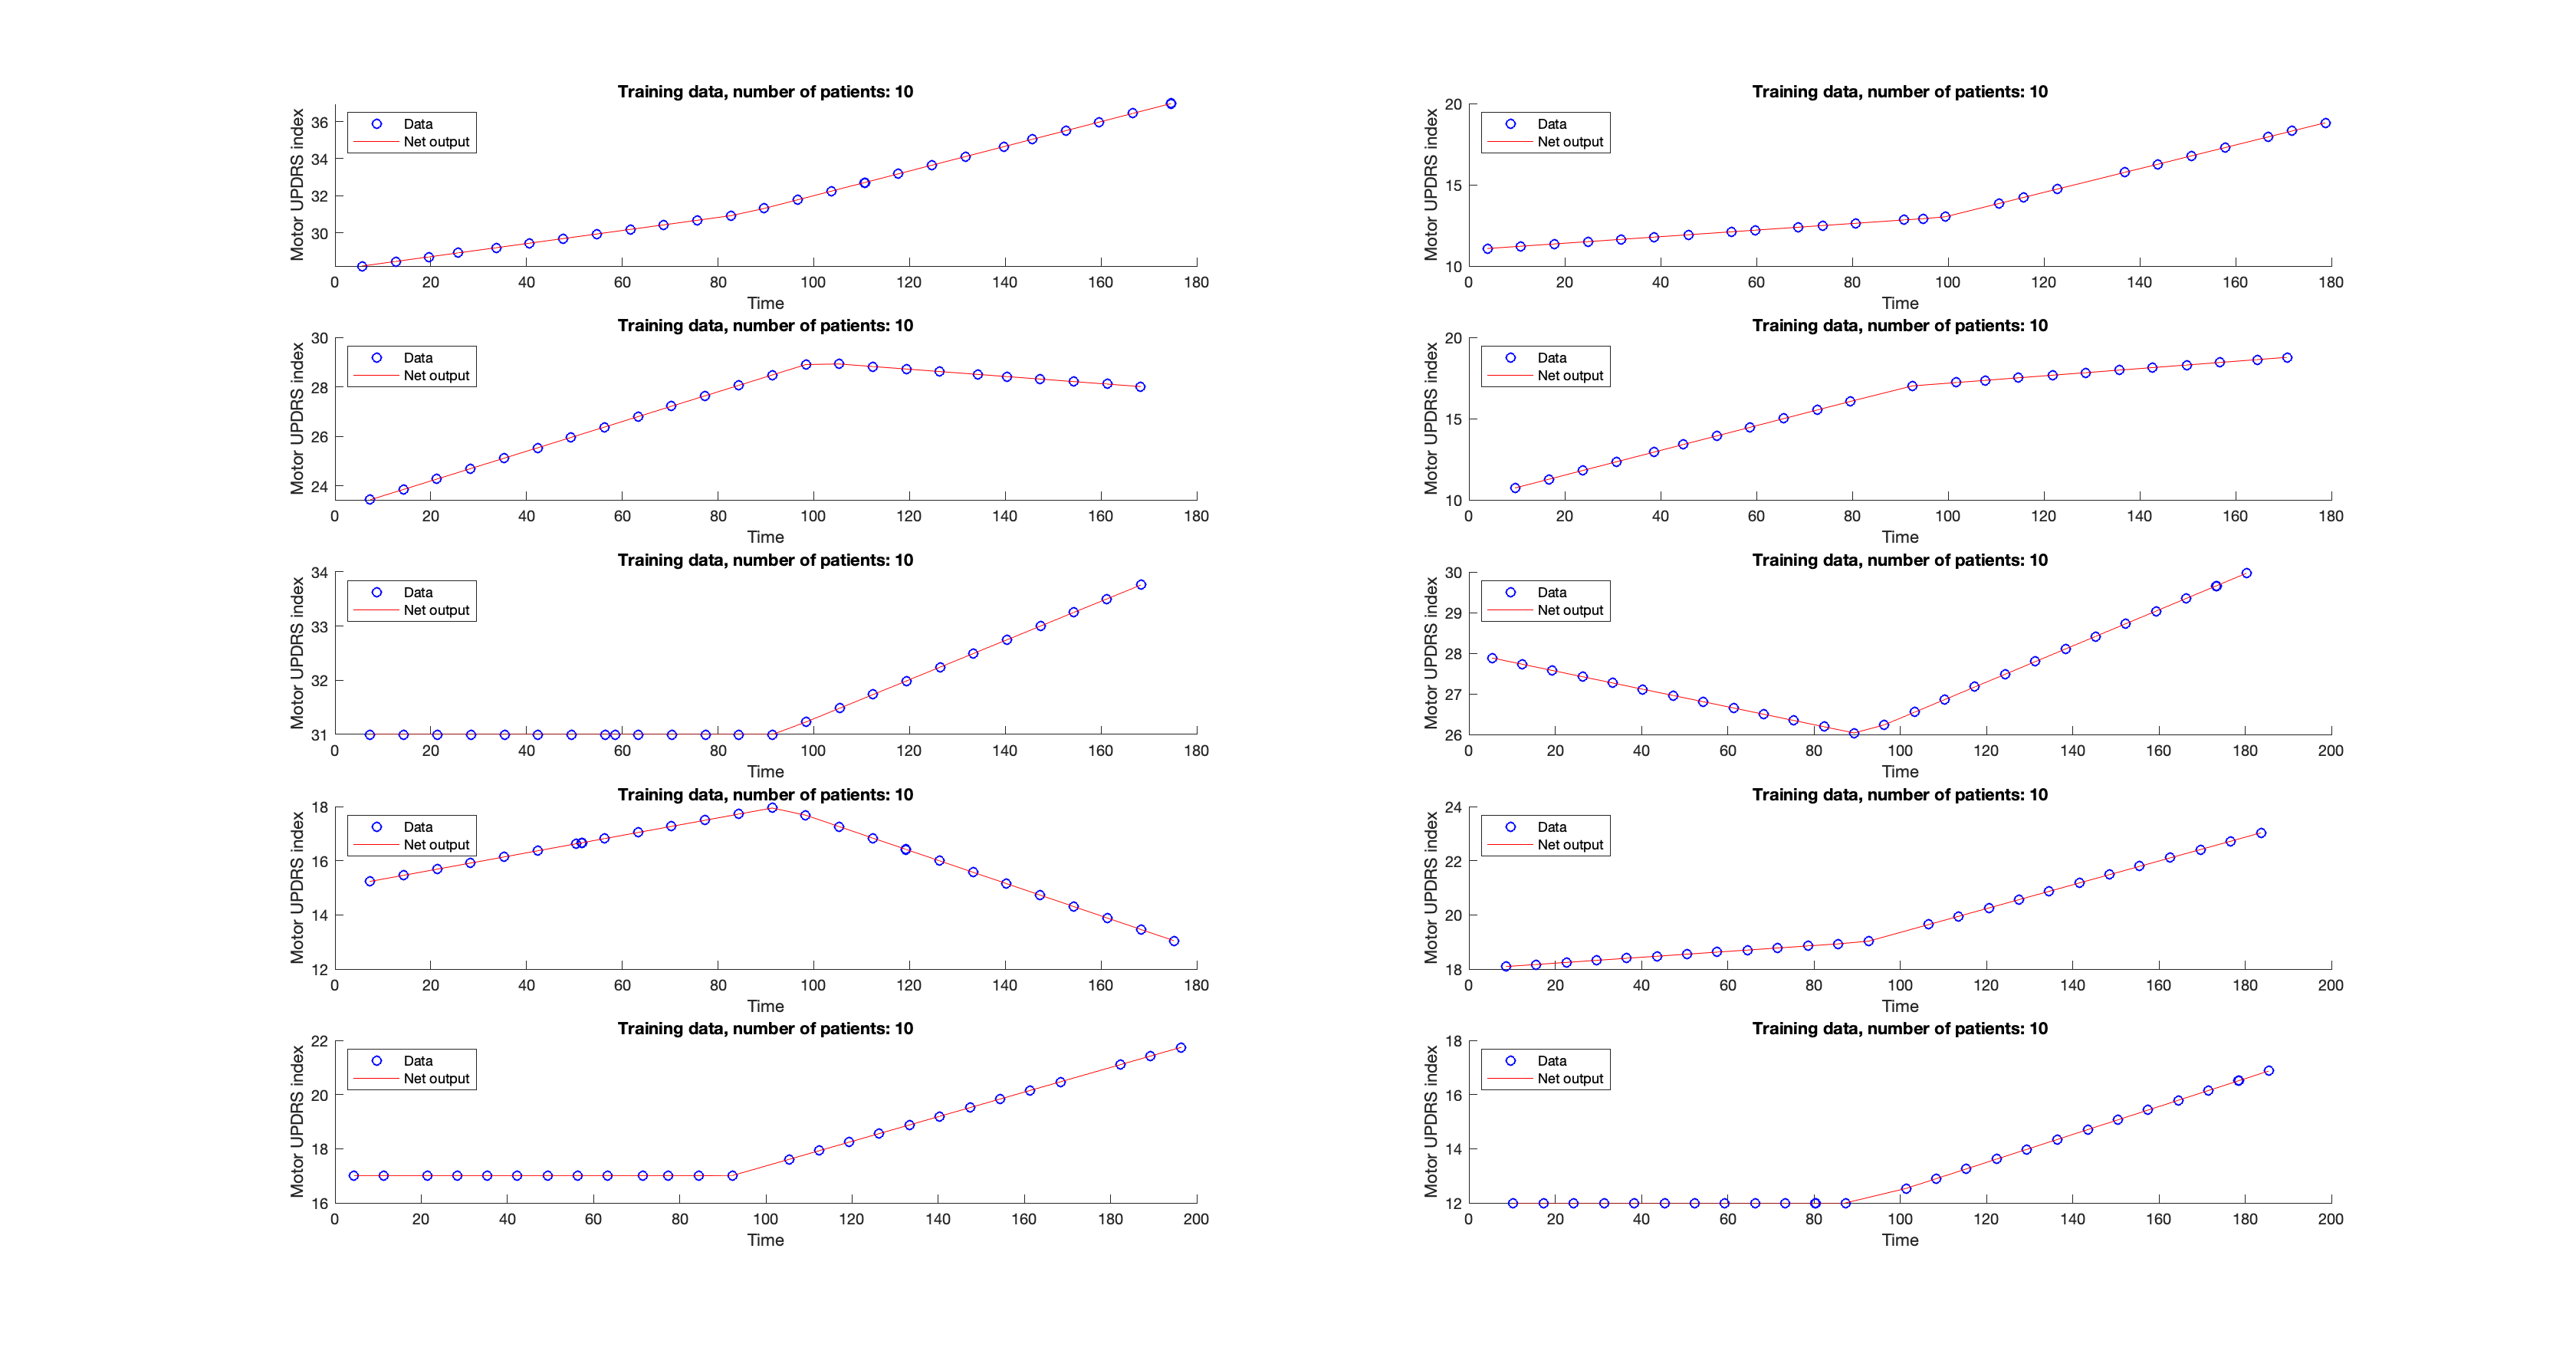
\includegraphics[width=1.1\textwidth]{training-normal-10.png}
\caption{Zbiór treningowy, 10 pacjentów}

\end{figure}

\begin{figure}[h!]

\centering
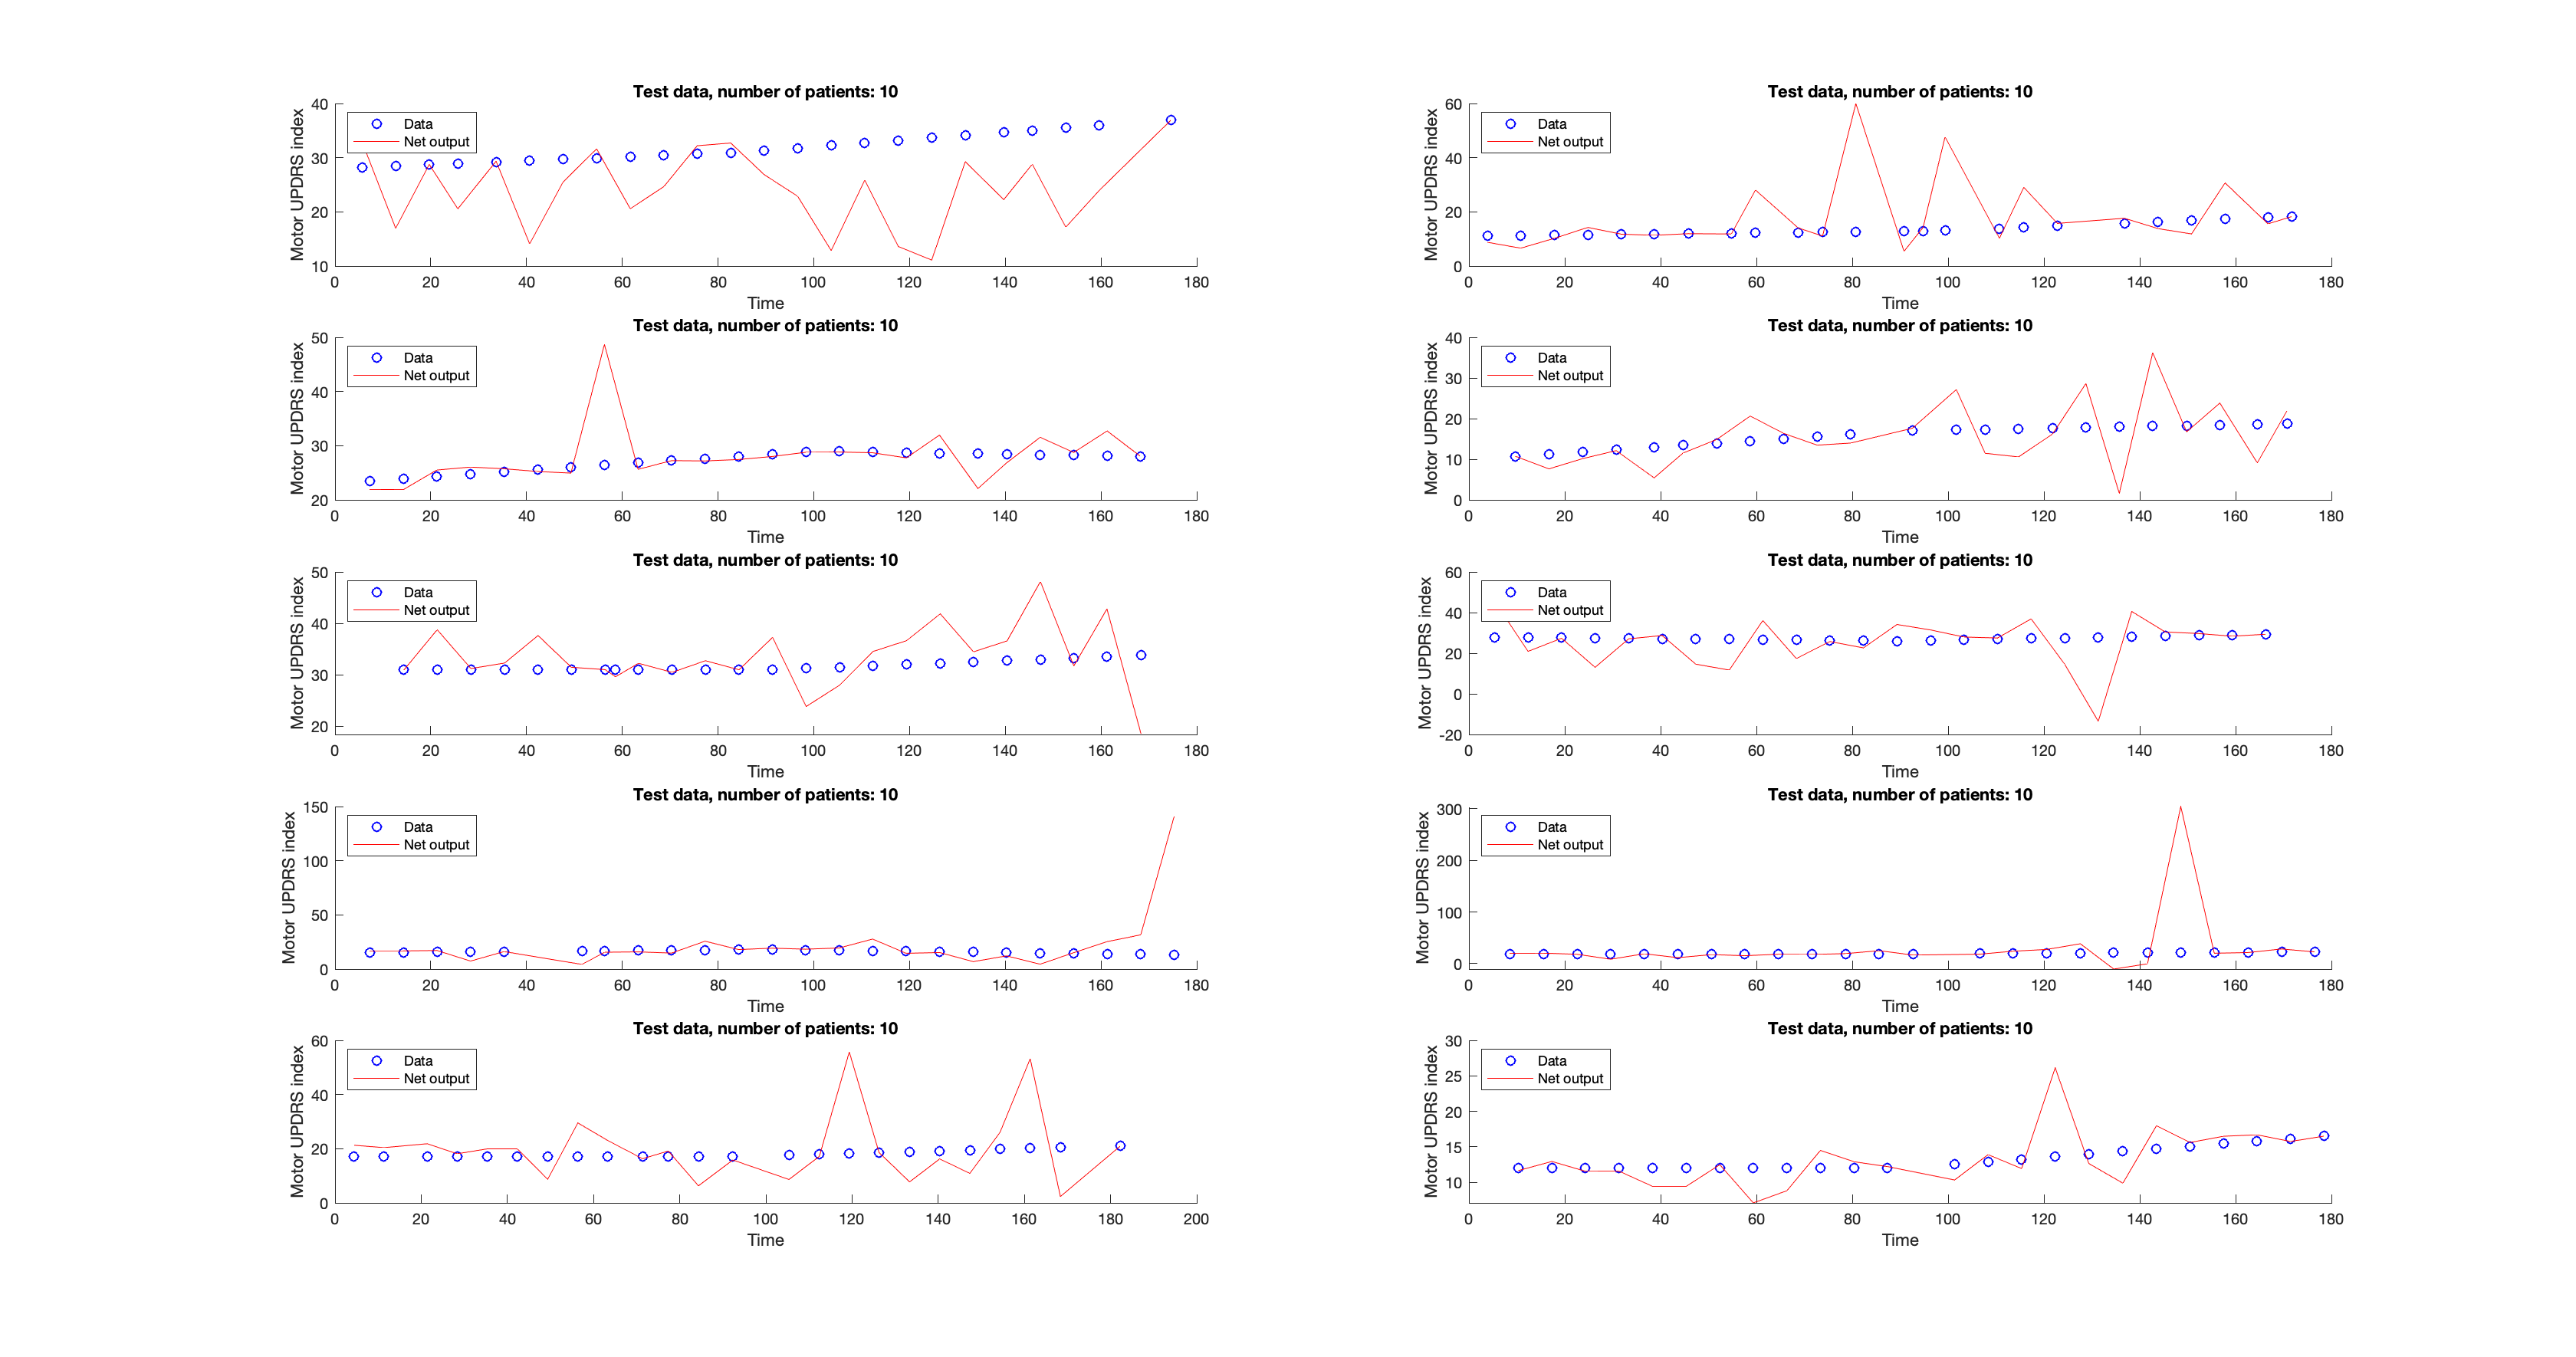
\includegraphics[width=1.1\textwidth]{test-normal-10.png}
\caption{Zbiór testowy, 10 pacjentów}

\end{figure}

\begin{figure}[h!]

\centering
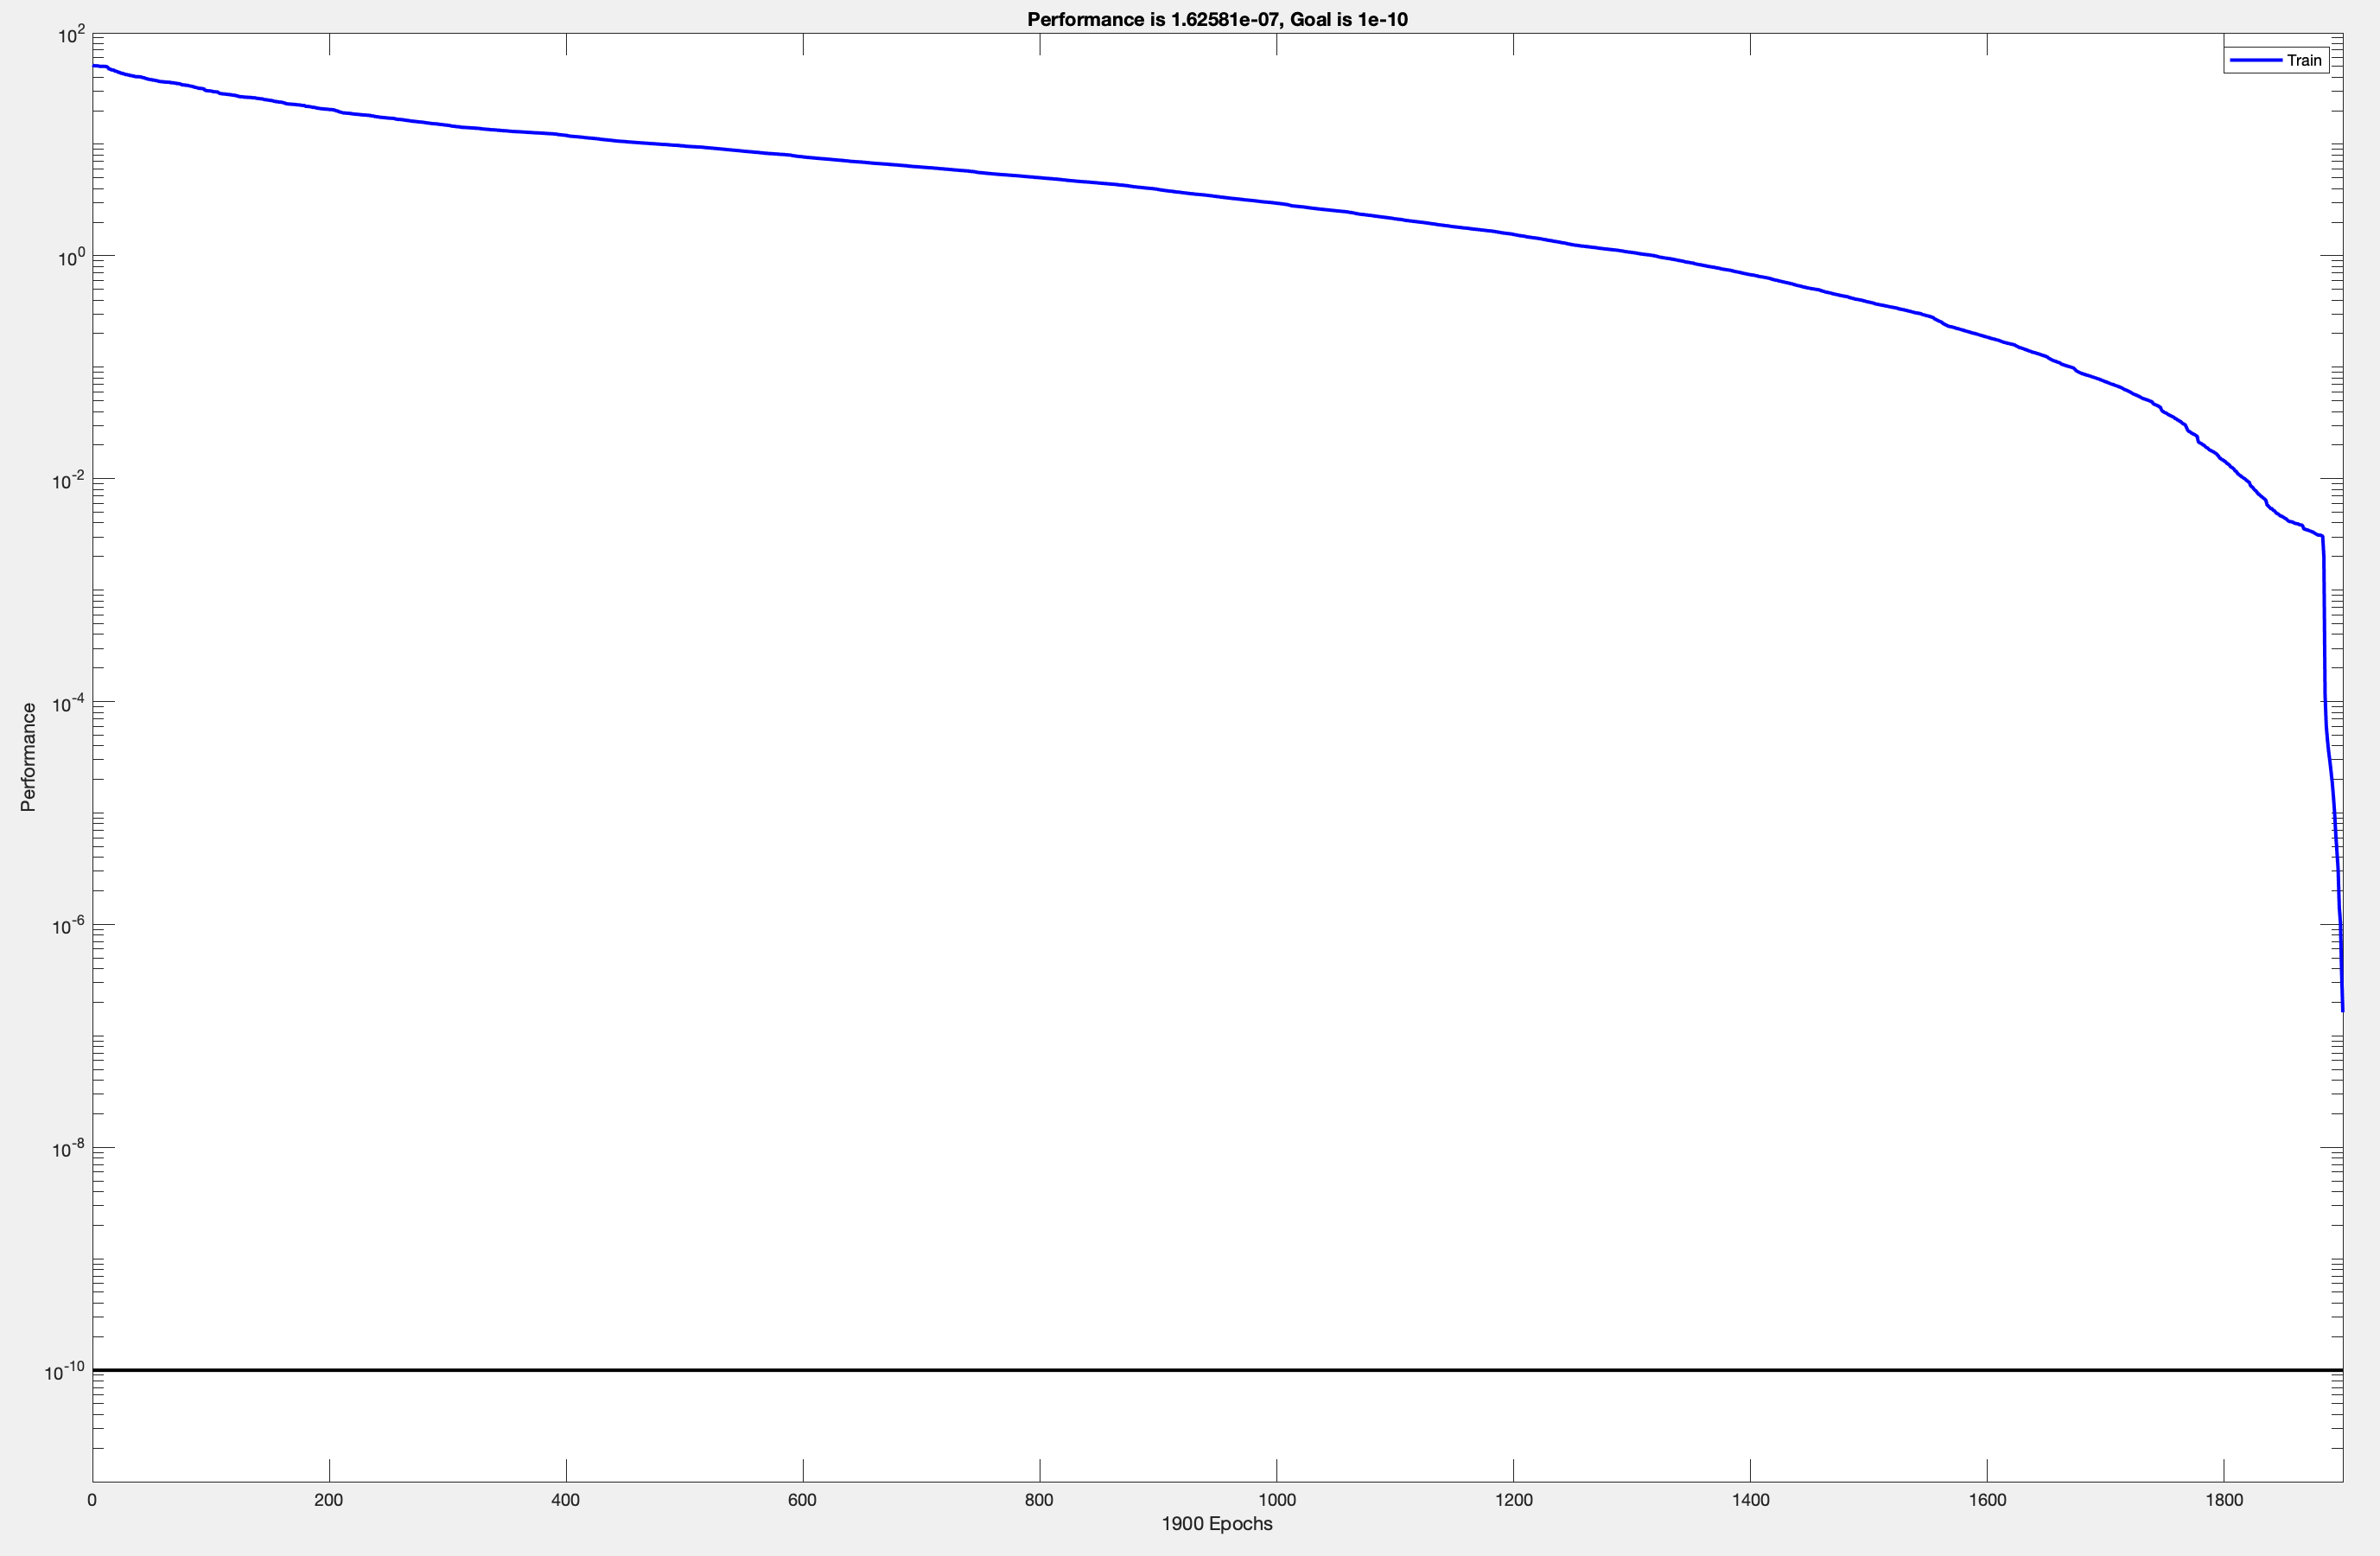
\includegraphics[width=0.9\textwidth]{mse-normal-16.png}
\caption{MSE dla 16 pacjentów}

\end{figure}

\begin{figure}[h!]

\centering
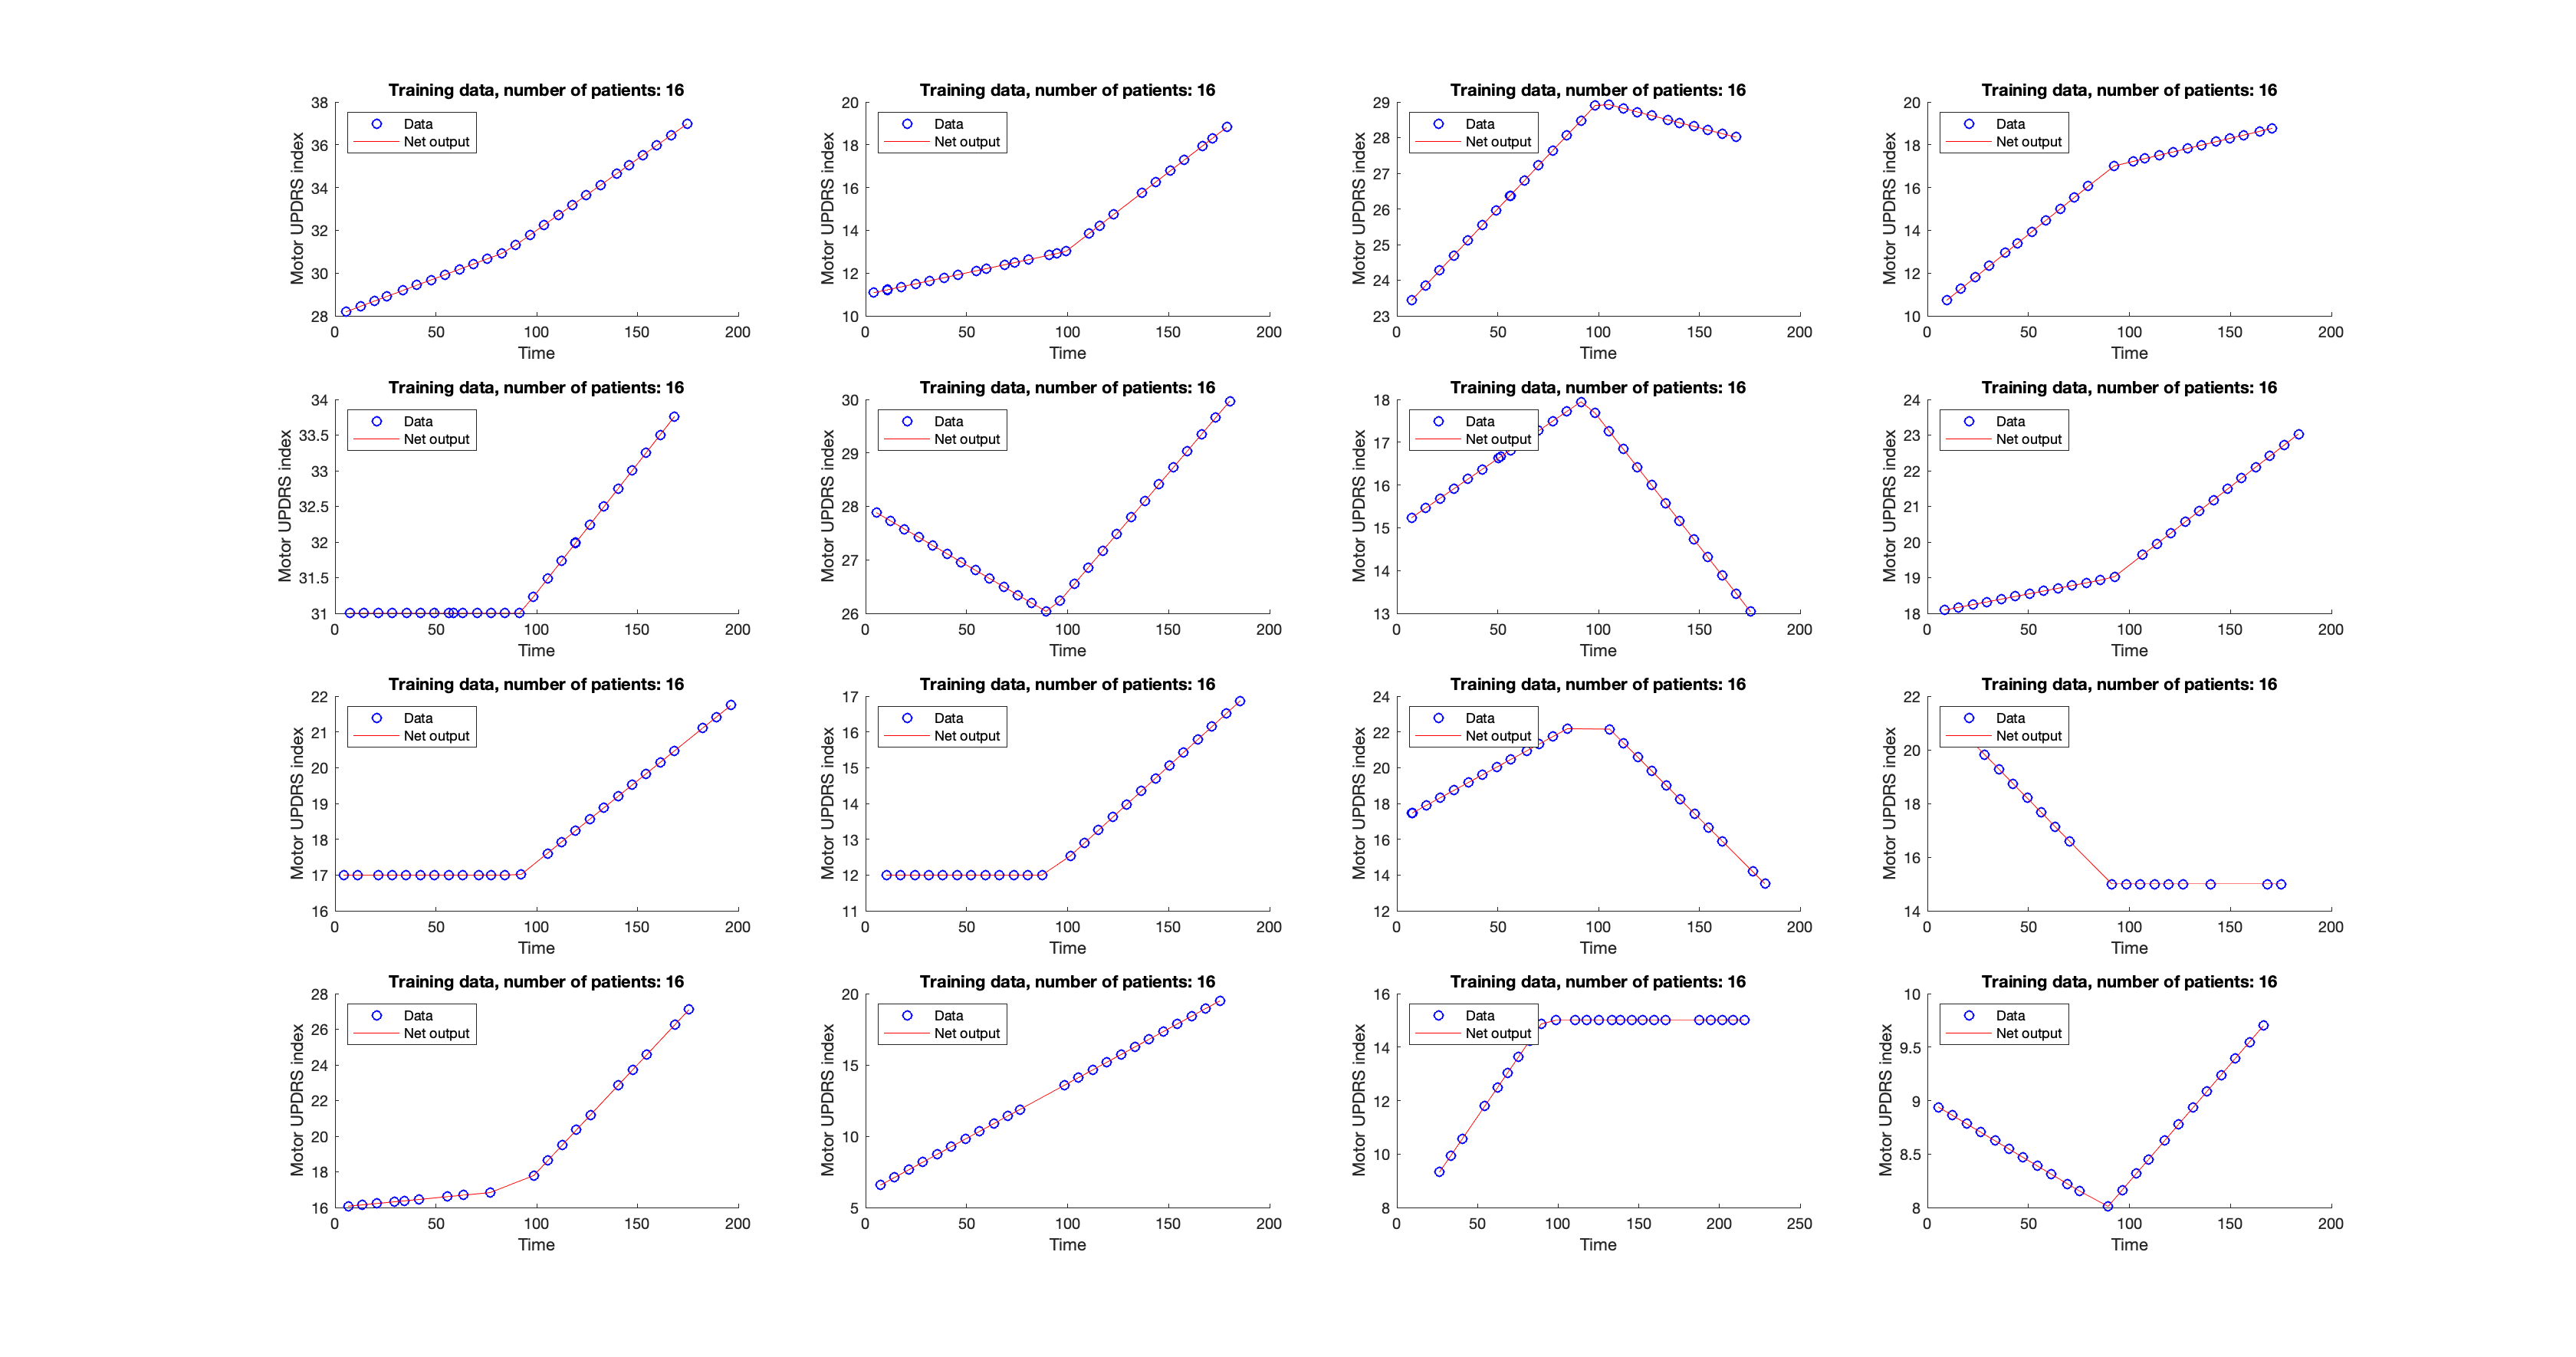
\includegraphics[width=1.1\textwidth]{training-normal-16.png}
\caption{Zbiór treningowy, 16 pacjentów}

\end{figure}

\begin{figure}[h!]

\centering
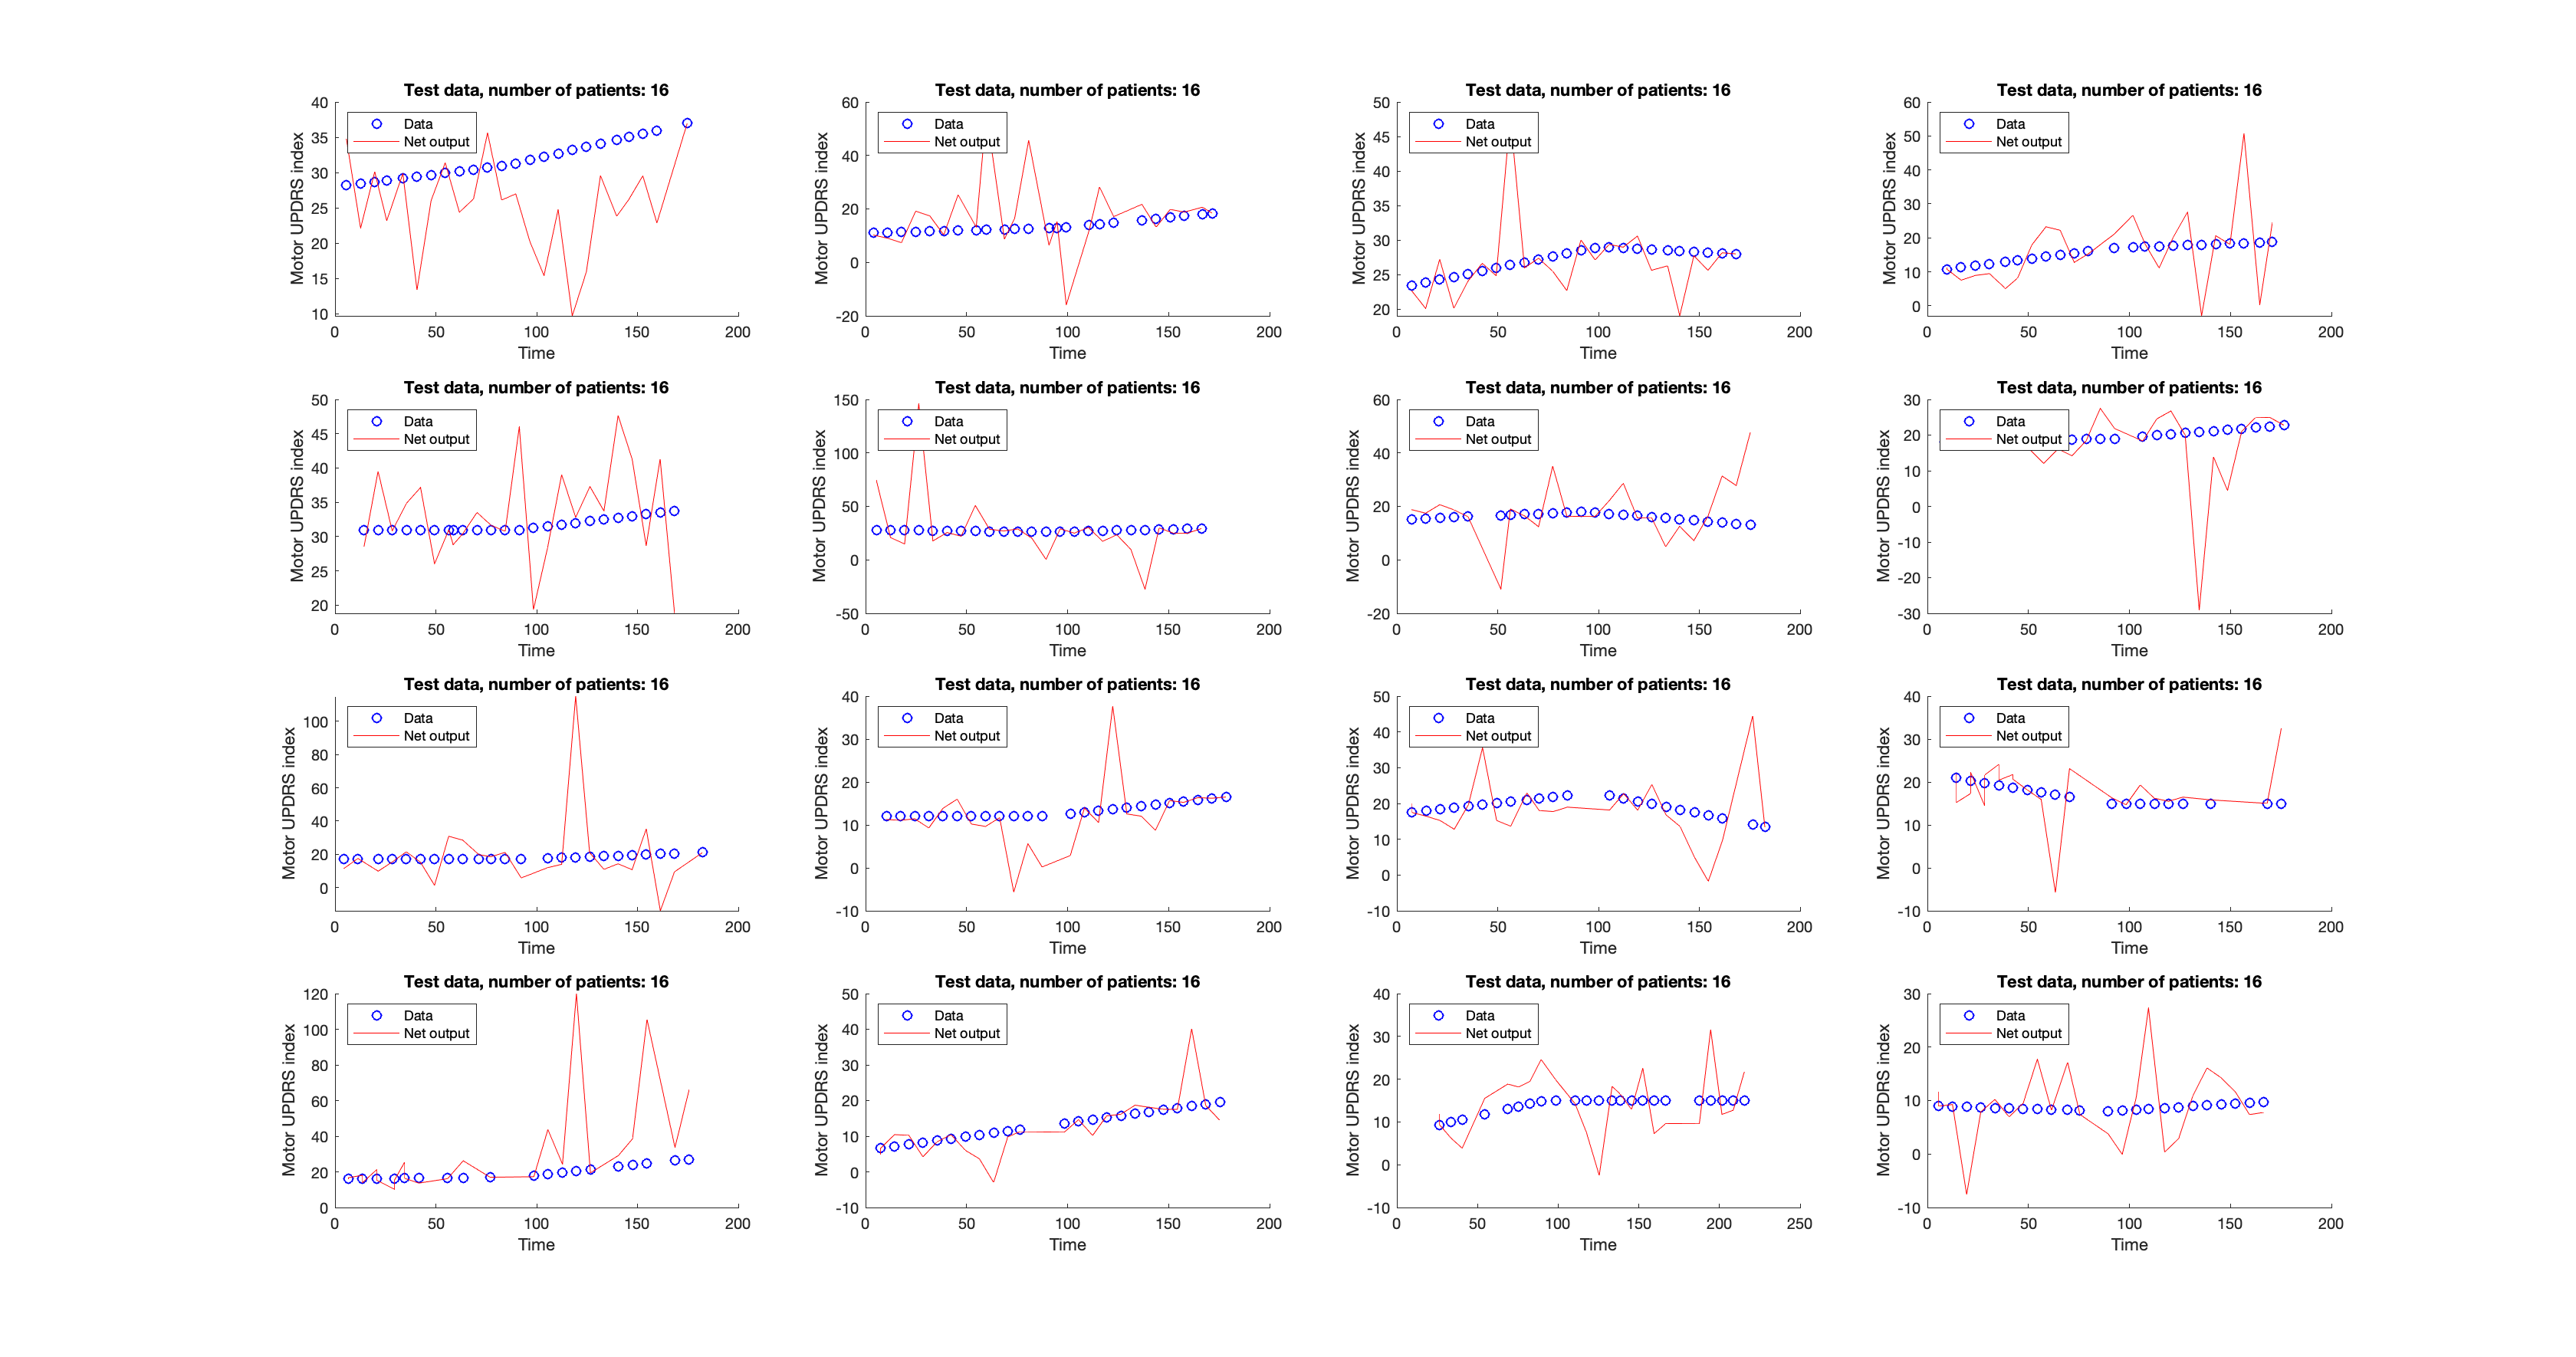
\includegraphics[width=1.2\textwidth]{test-normal-16.png}
\caption{Zbiór testowy, 16 pacjentów}

\end{figure}

\newpage

Przy zwiększonej ilości pacjentów oraz dużej ilości danych uczących sieć wykazuje pewne problemy z nauką. Znacząco wydłuża się czas uczenia, można także zaobserwować pogorszenie jakości wykonywanej predykcji. Testy dla maksymalnej liczby pacjentów nie zostały wykonane ze względu na czas uczenia przekraczający kilka godzin.

\subsection{Dane bez duplikatów próbek czasowych z małą ilością pacjentów}

Parametry uczenia:
\begin{itemize}
\item Mean squared error: $10^{-9}$
\item Spread constant: $50$
\end{itemize}

\begin{figure}[h!]

\centering
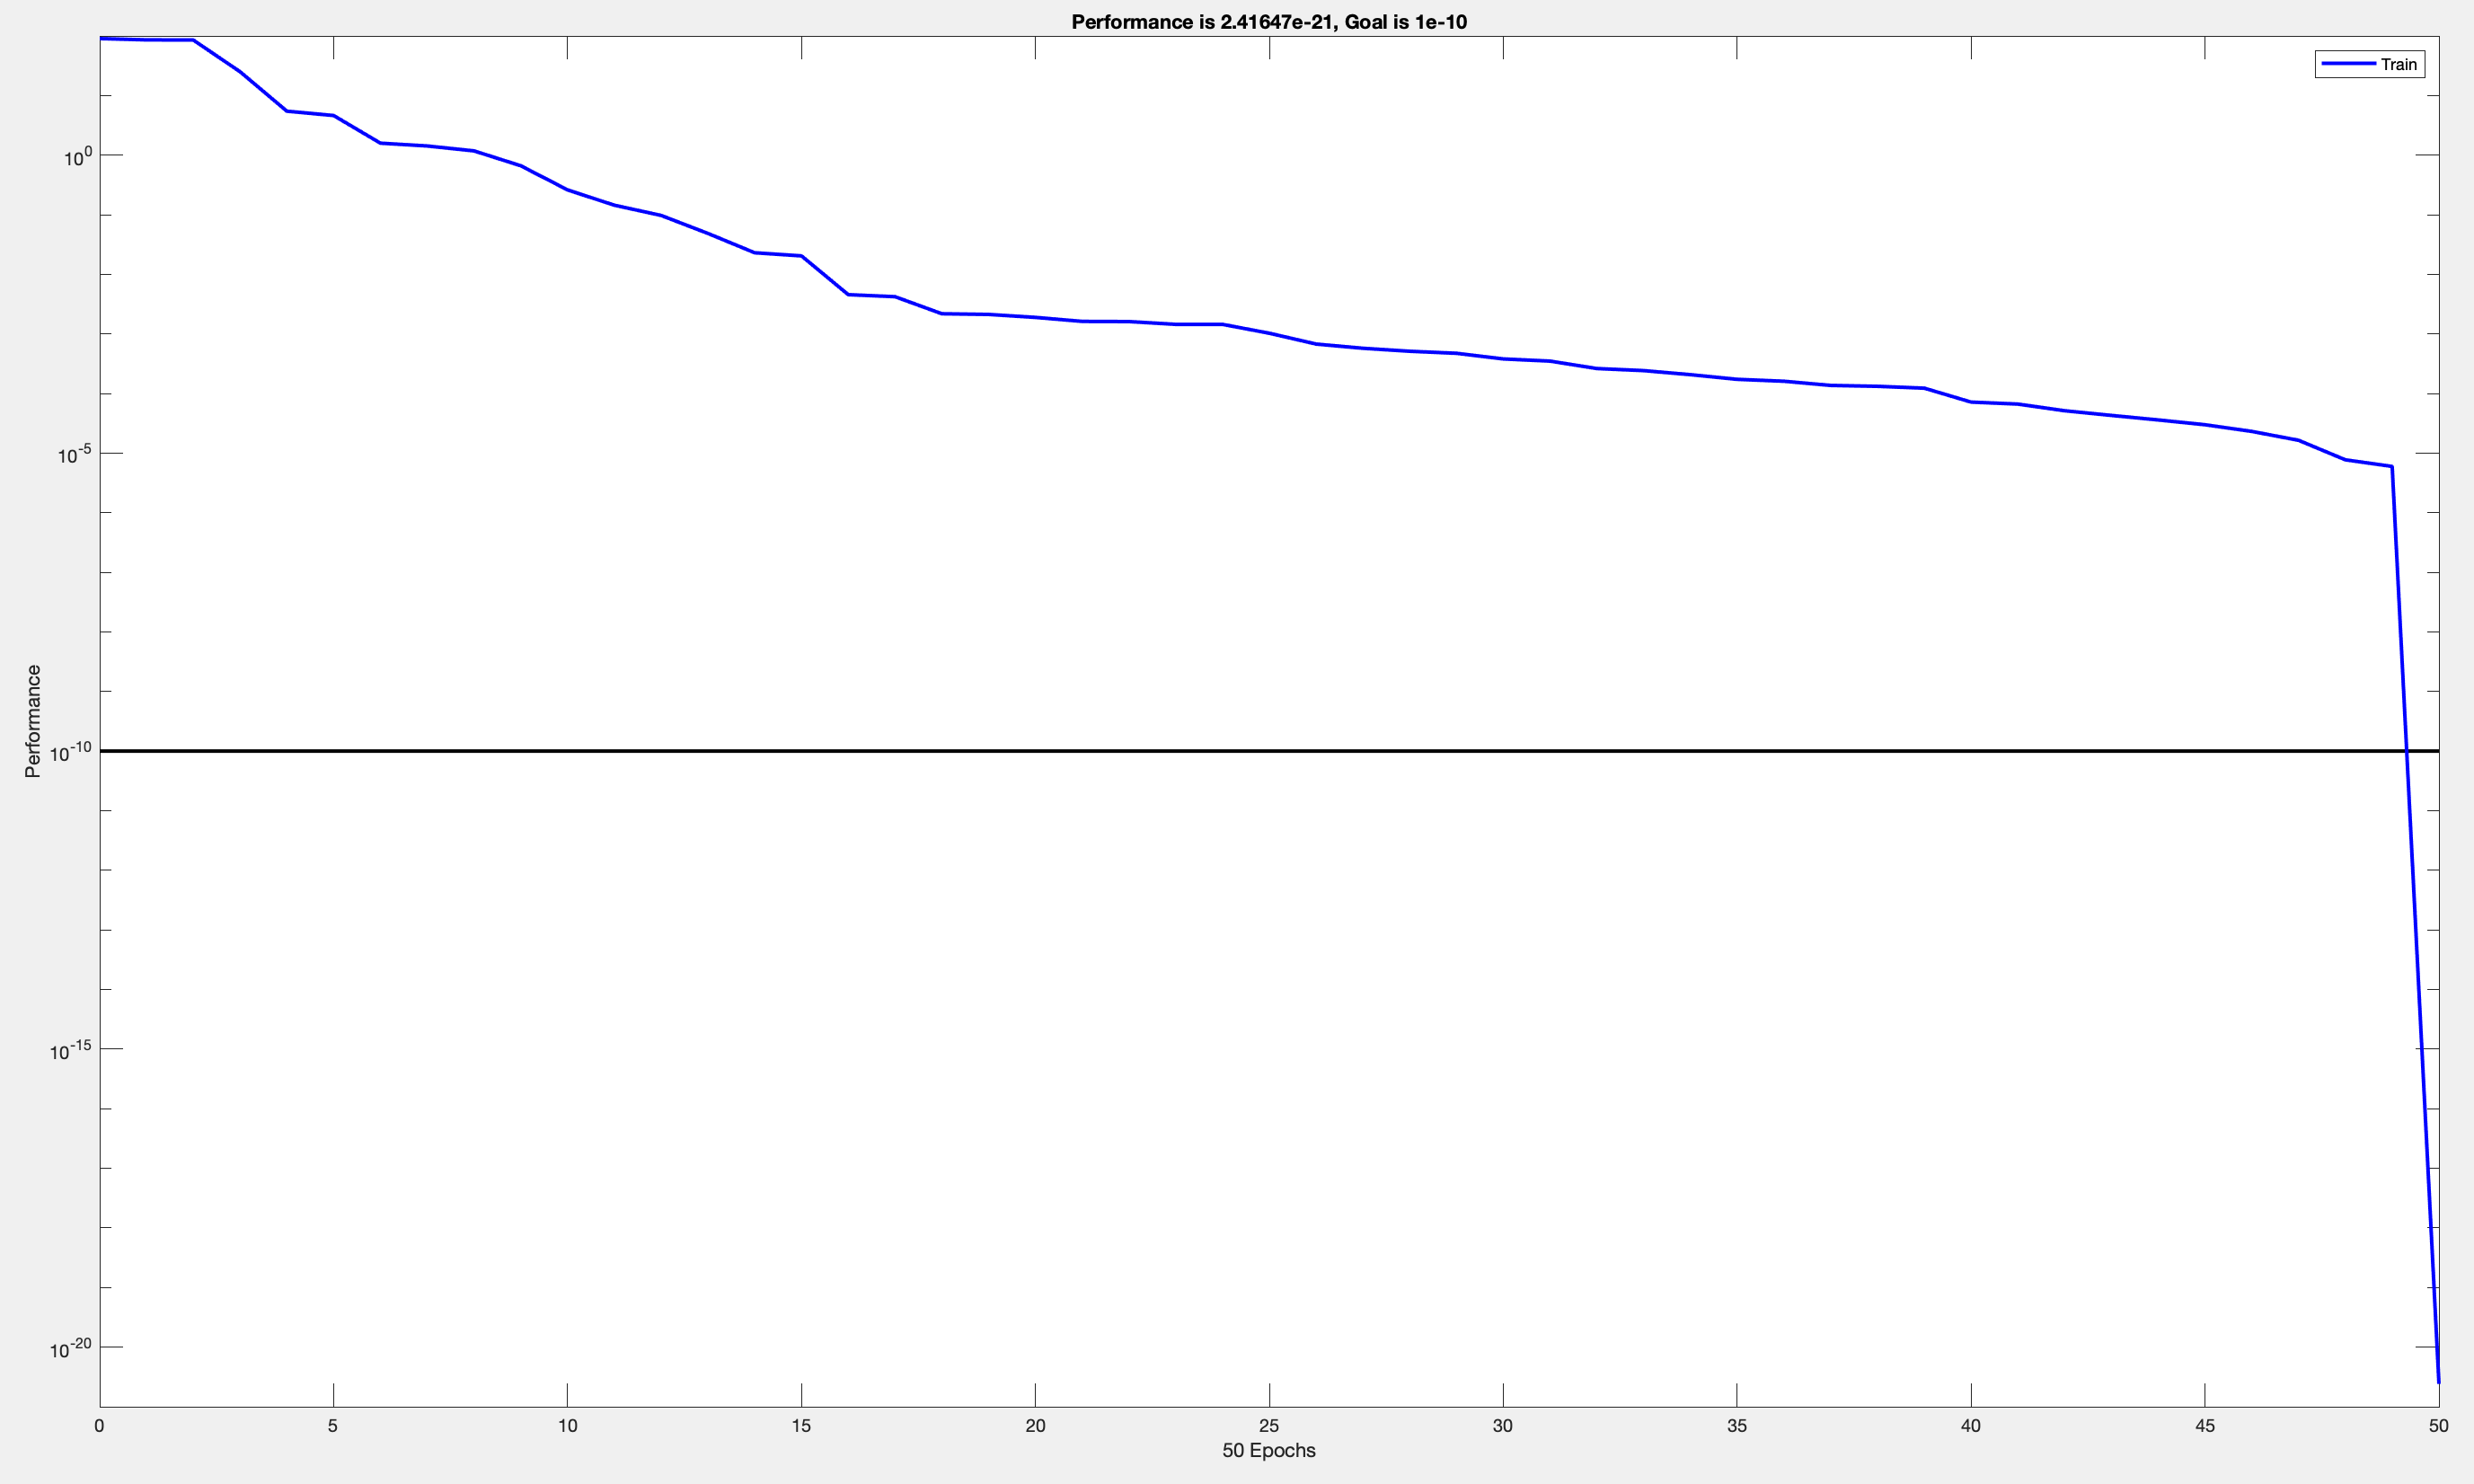
\includegraphics[width=1.0\textwidth]{mse-cut-2.png}
\caption{MSE dla 2 pacjentów}

\end{figure}

\begin{figure}[h!]

\centering
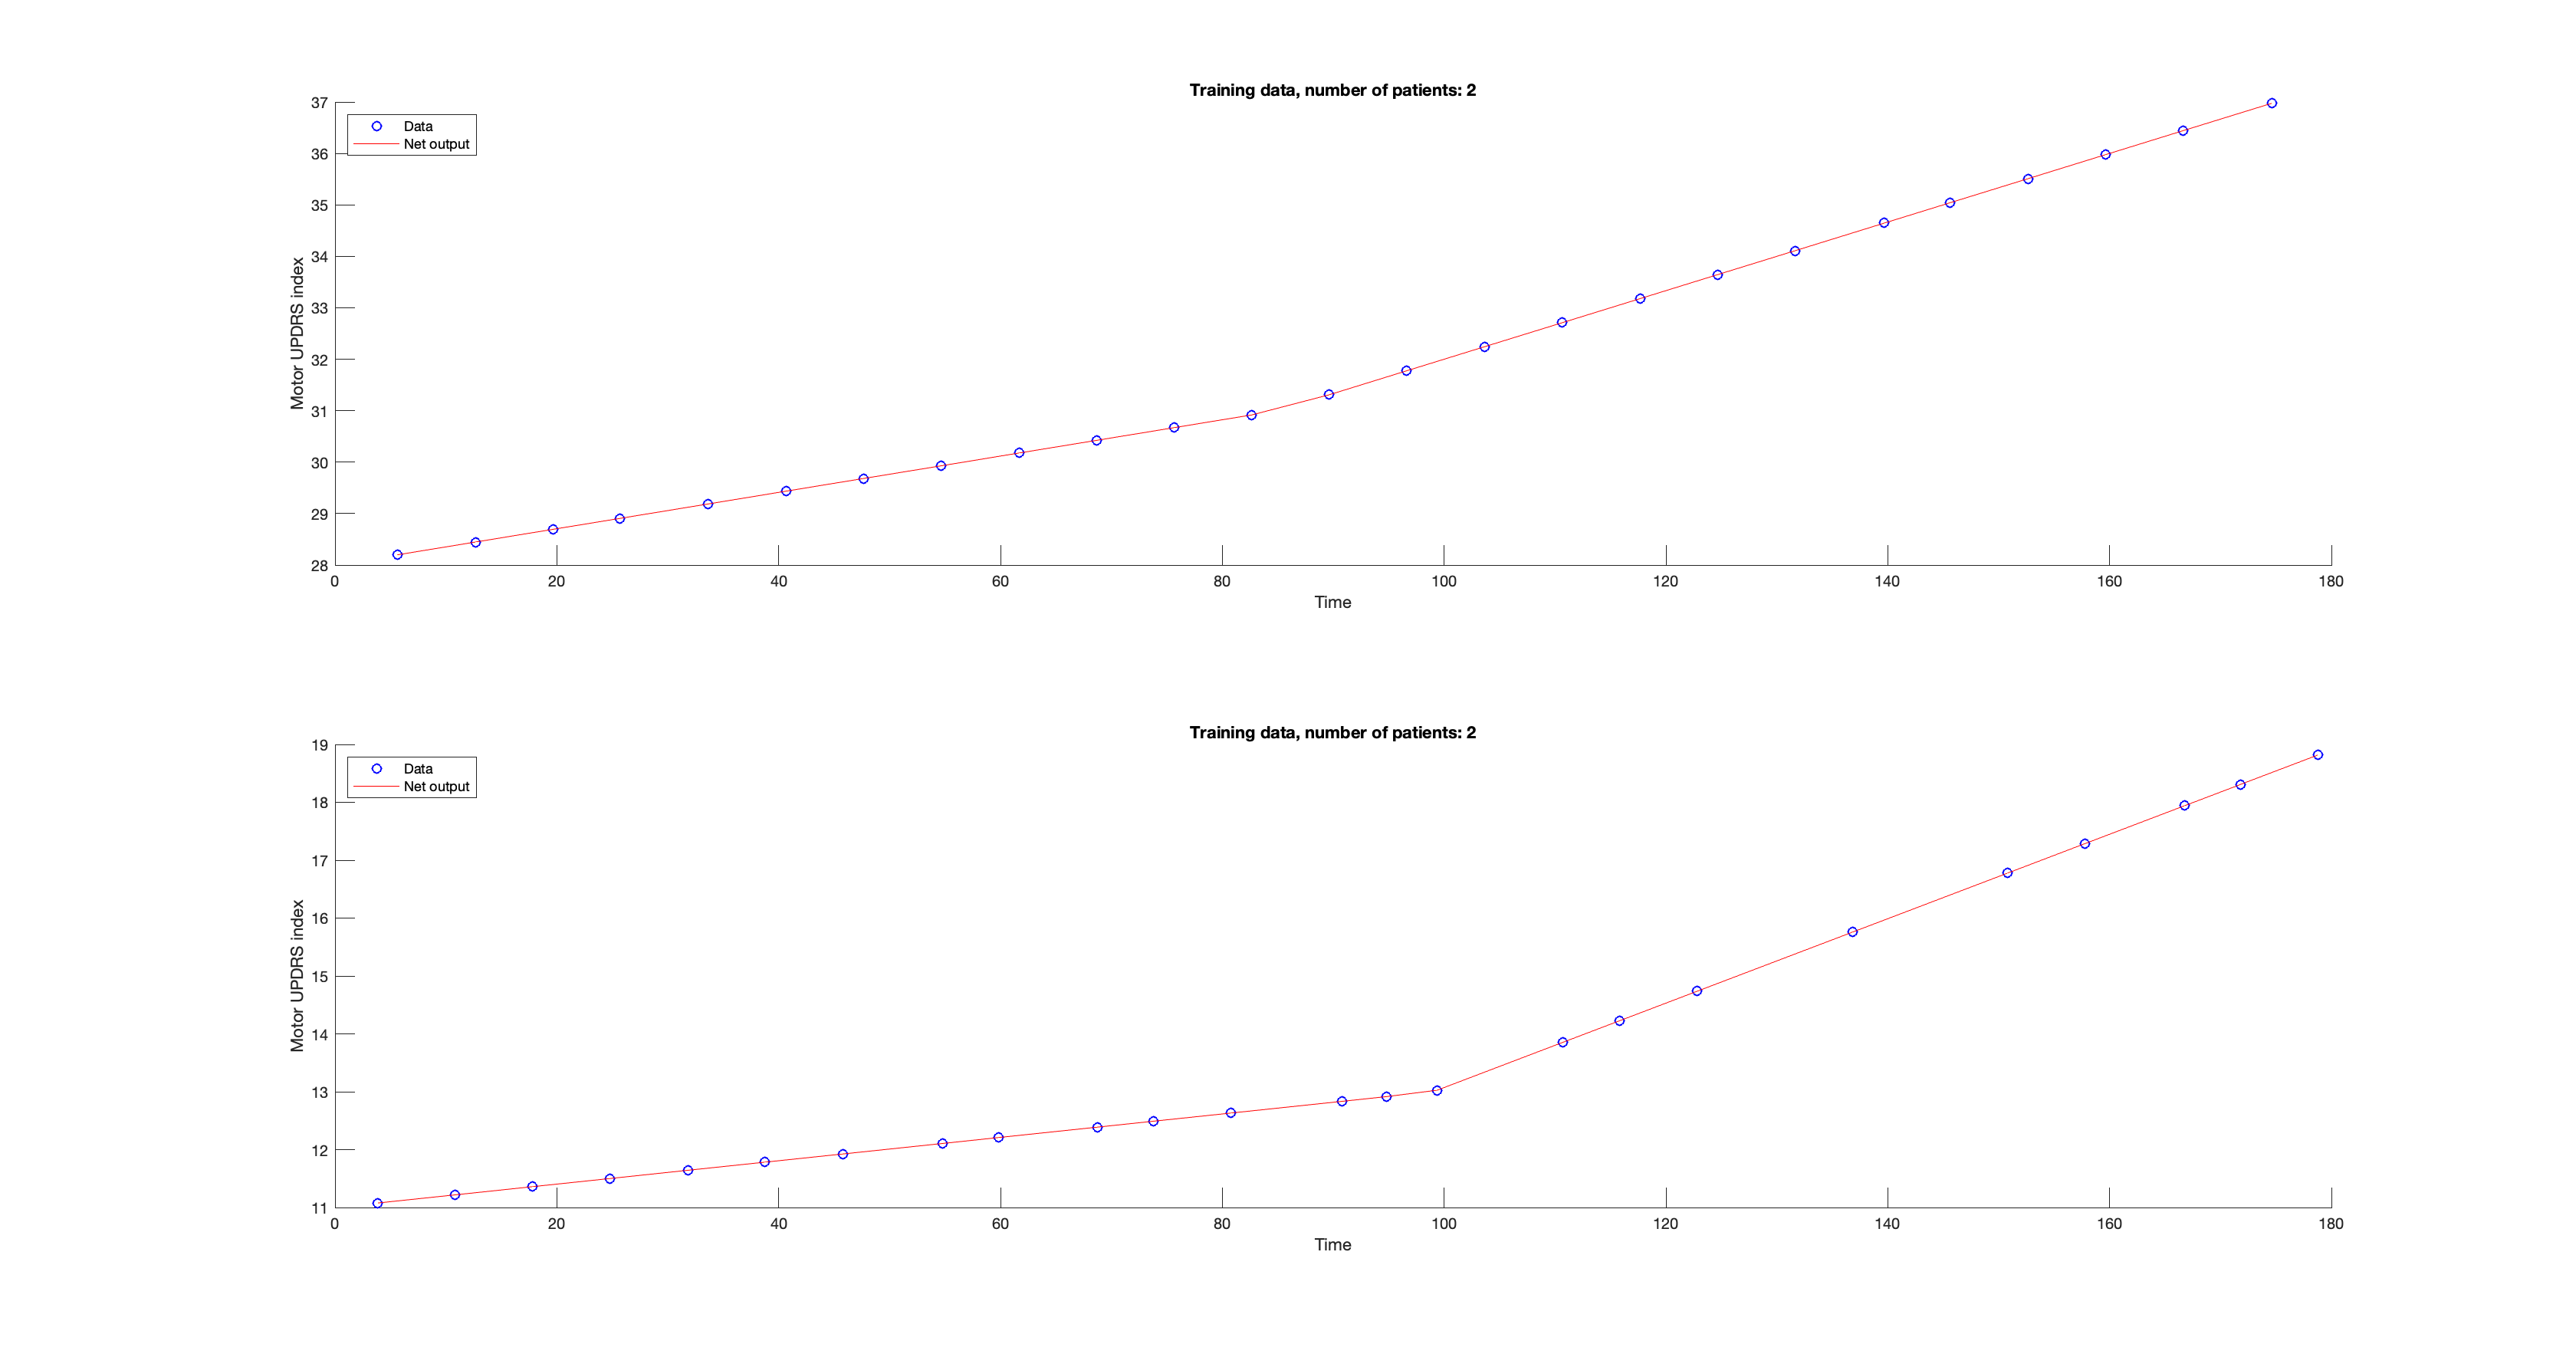
\includegraphics[width=1.05\textwidth]{training-cut-2.png}
\caption{Zbiór treningowy, 2 pacjentów}

\end{figure}

\begin{figure}[h!]

\centering
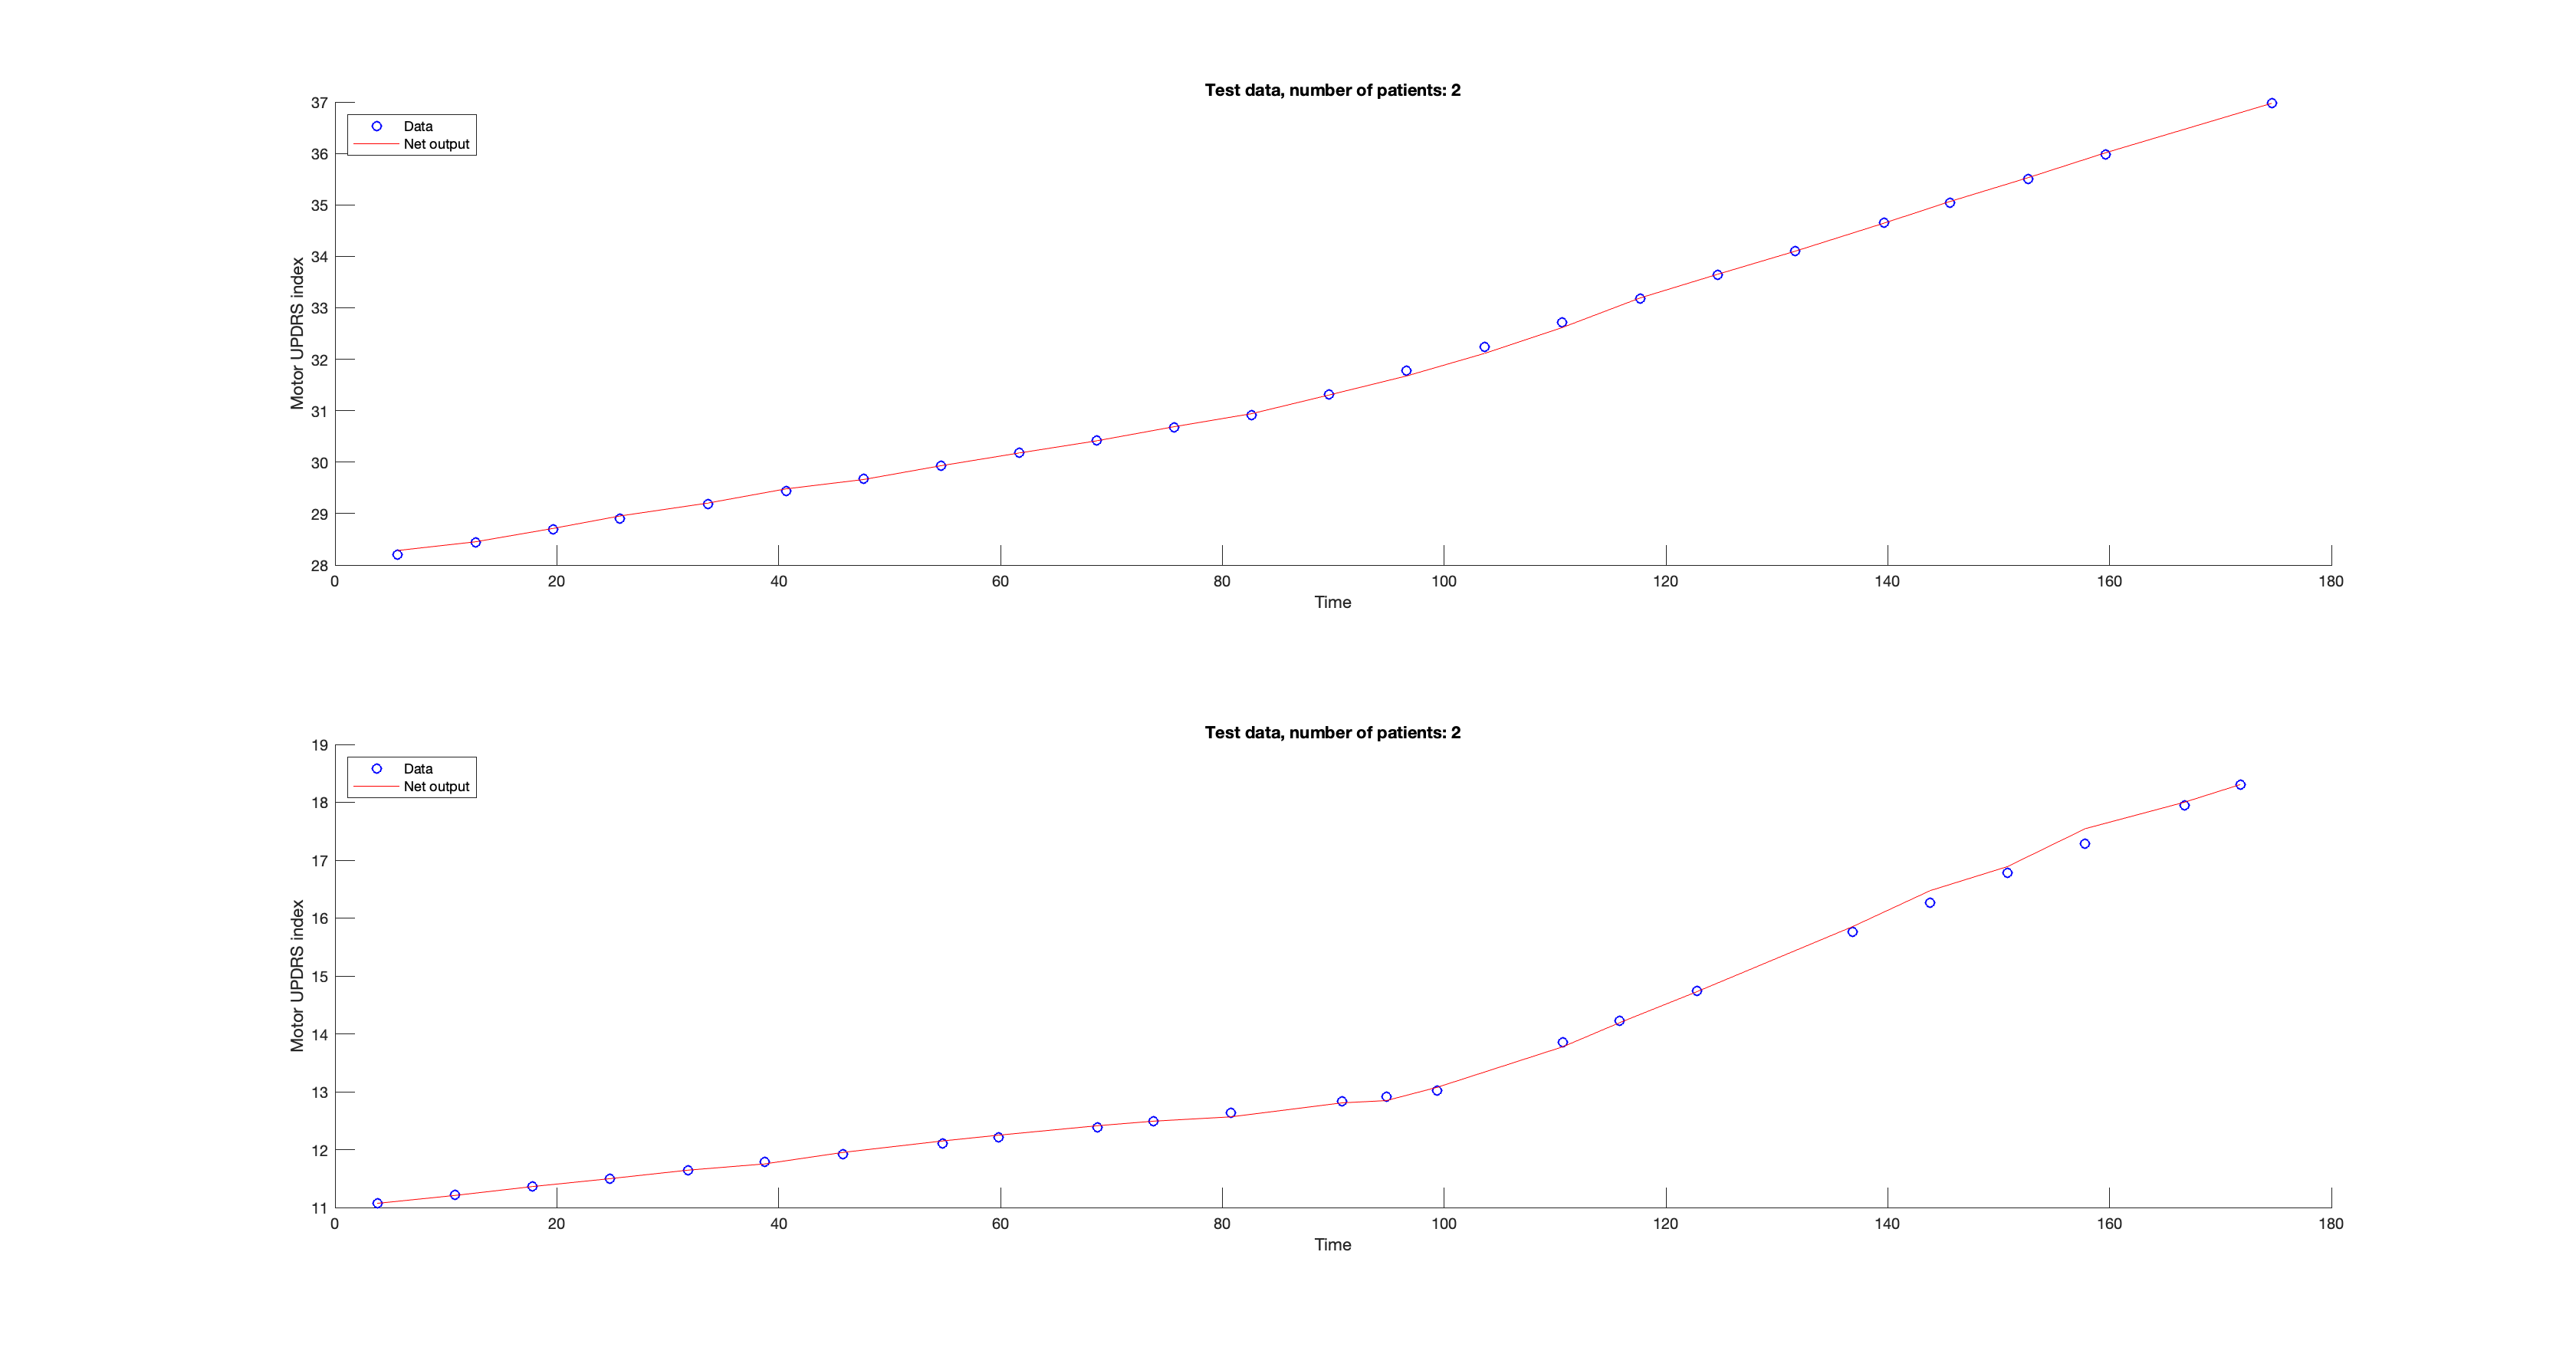
\includegraphics[width=1.0\textwidth]{test-cut-2.png}
\caption{Zbiór testowy, 2 pacjentów}

\end{figure}

\begin{figure}[h!]

\centering
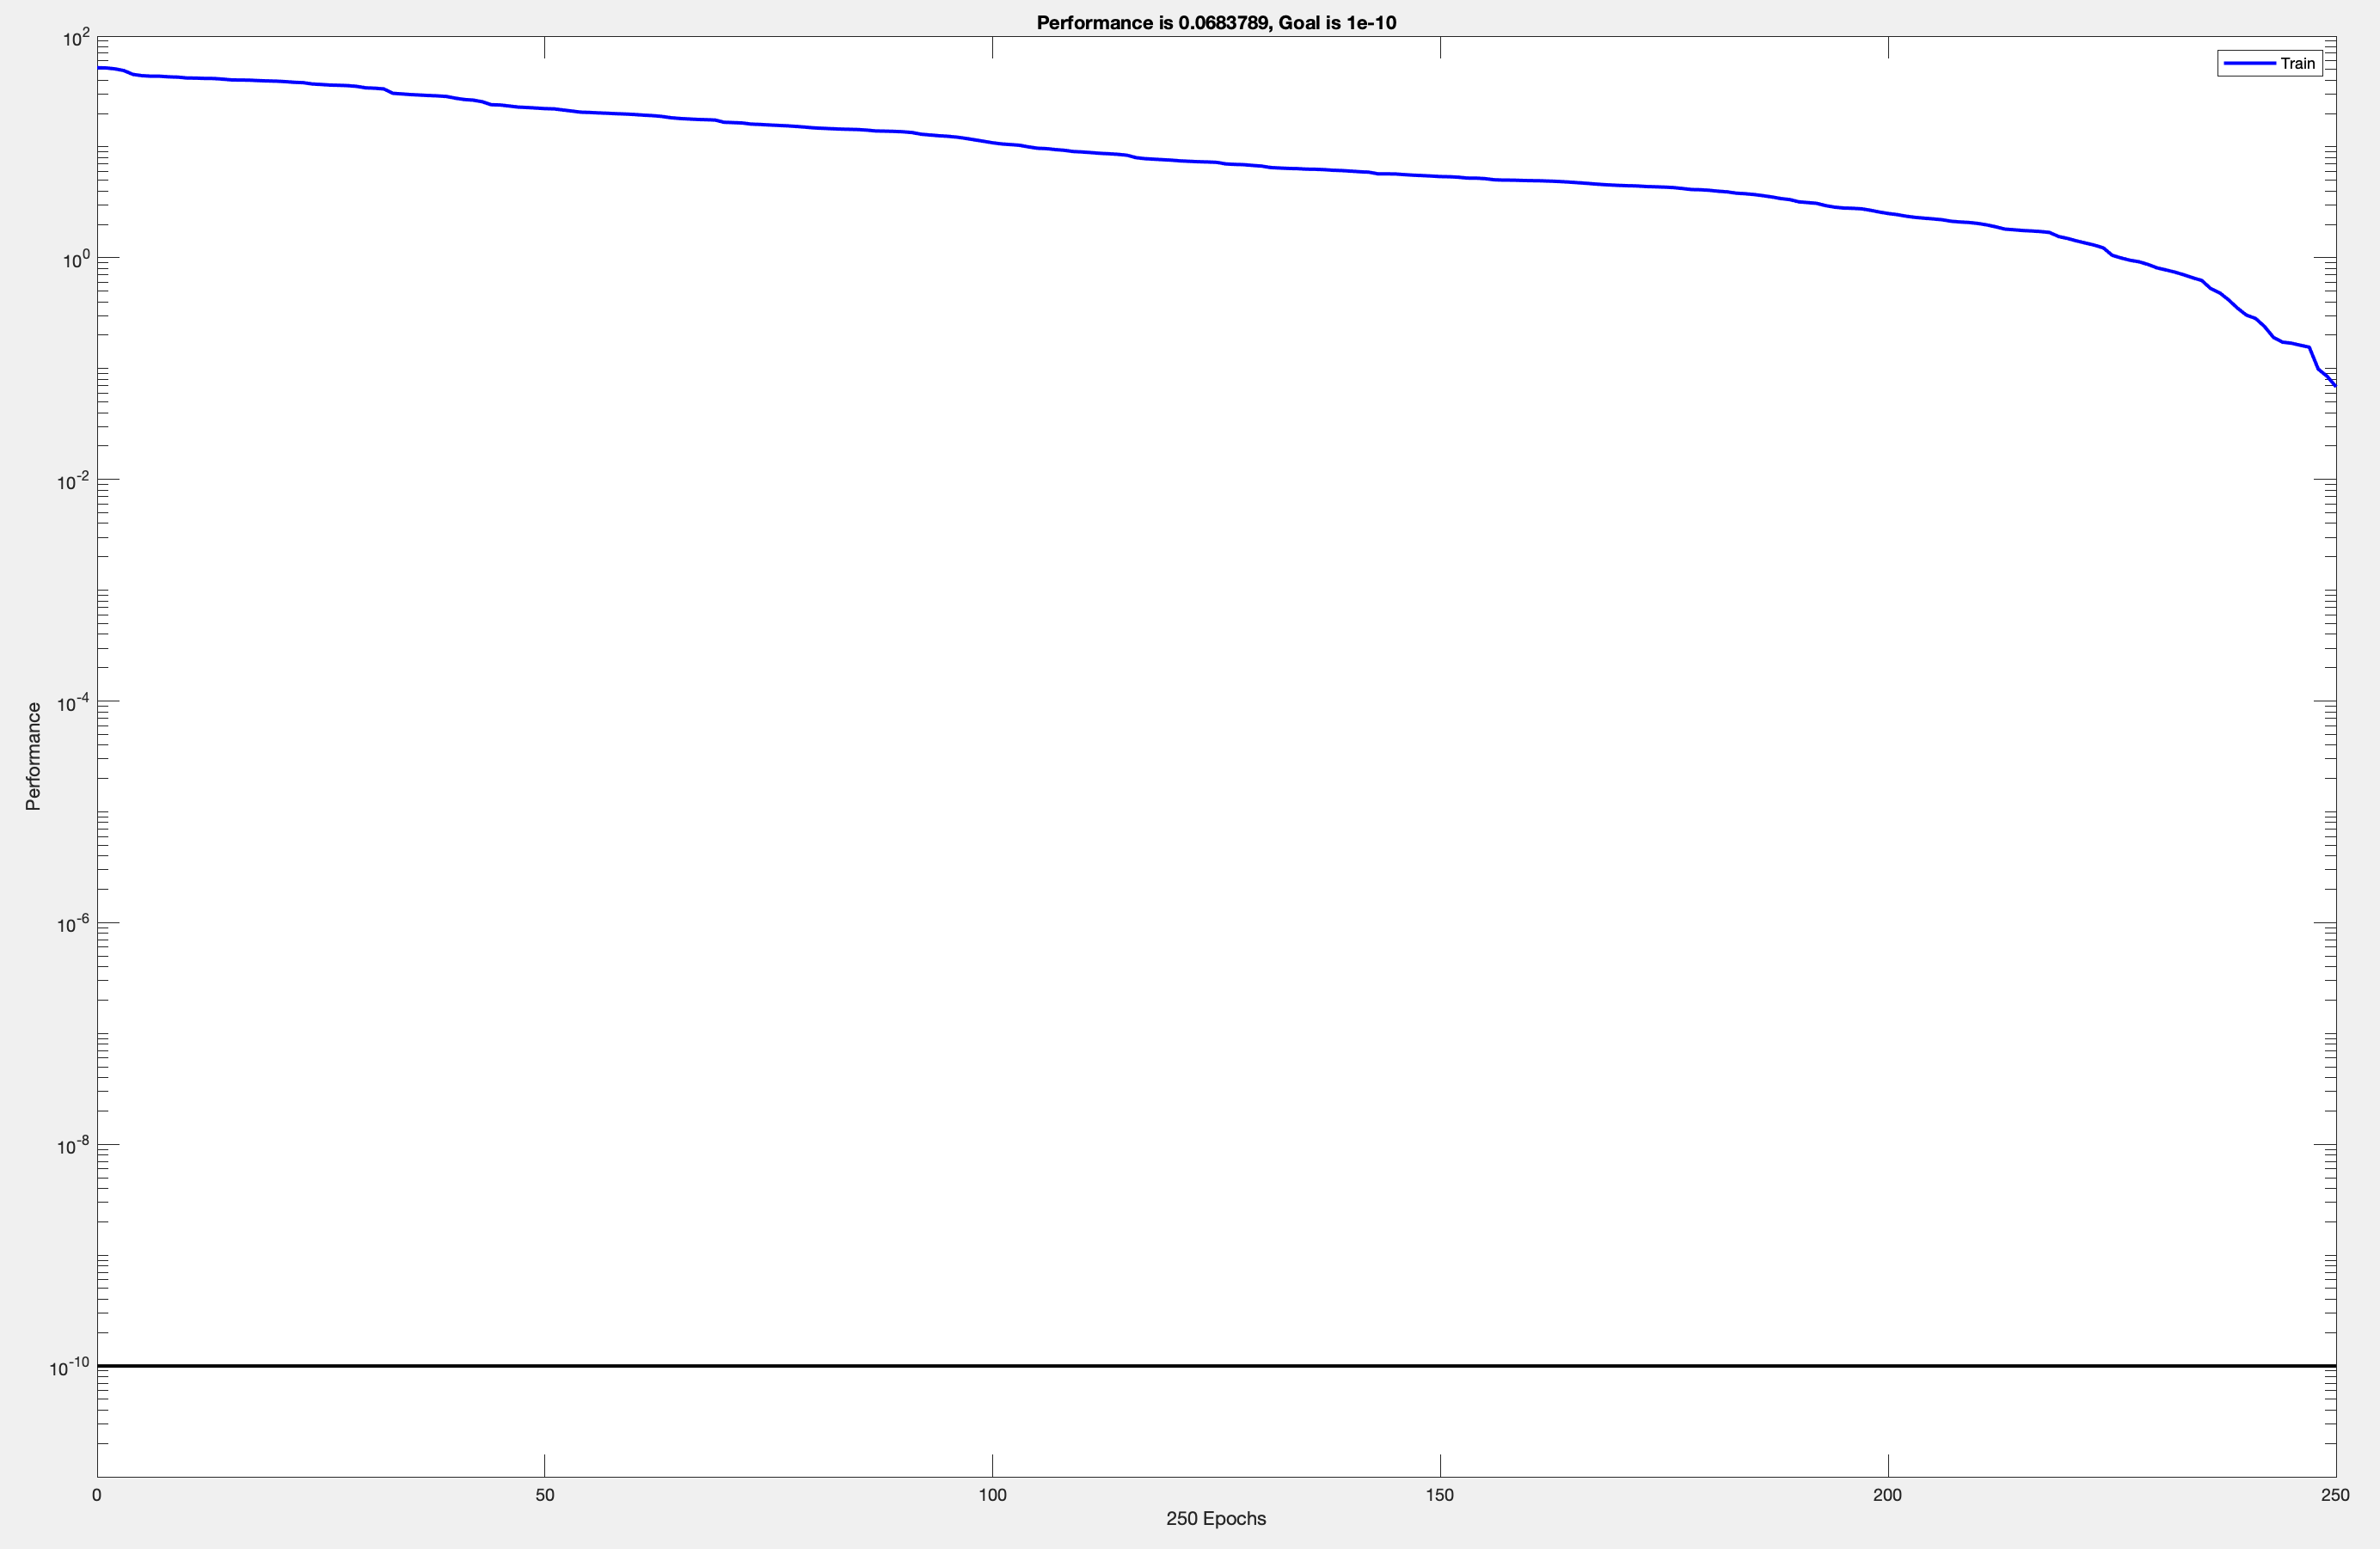
\includegraphics[width=1.0\textwidth]{mse-cut-10.png}
\caption{MSE dla 10 pacjentów}

\end{figure}

\begin{figure}[h!]

\centering
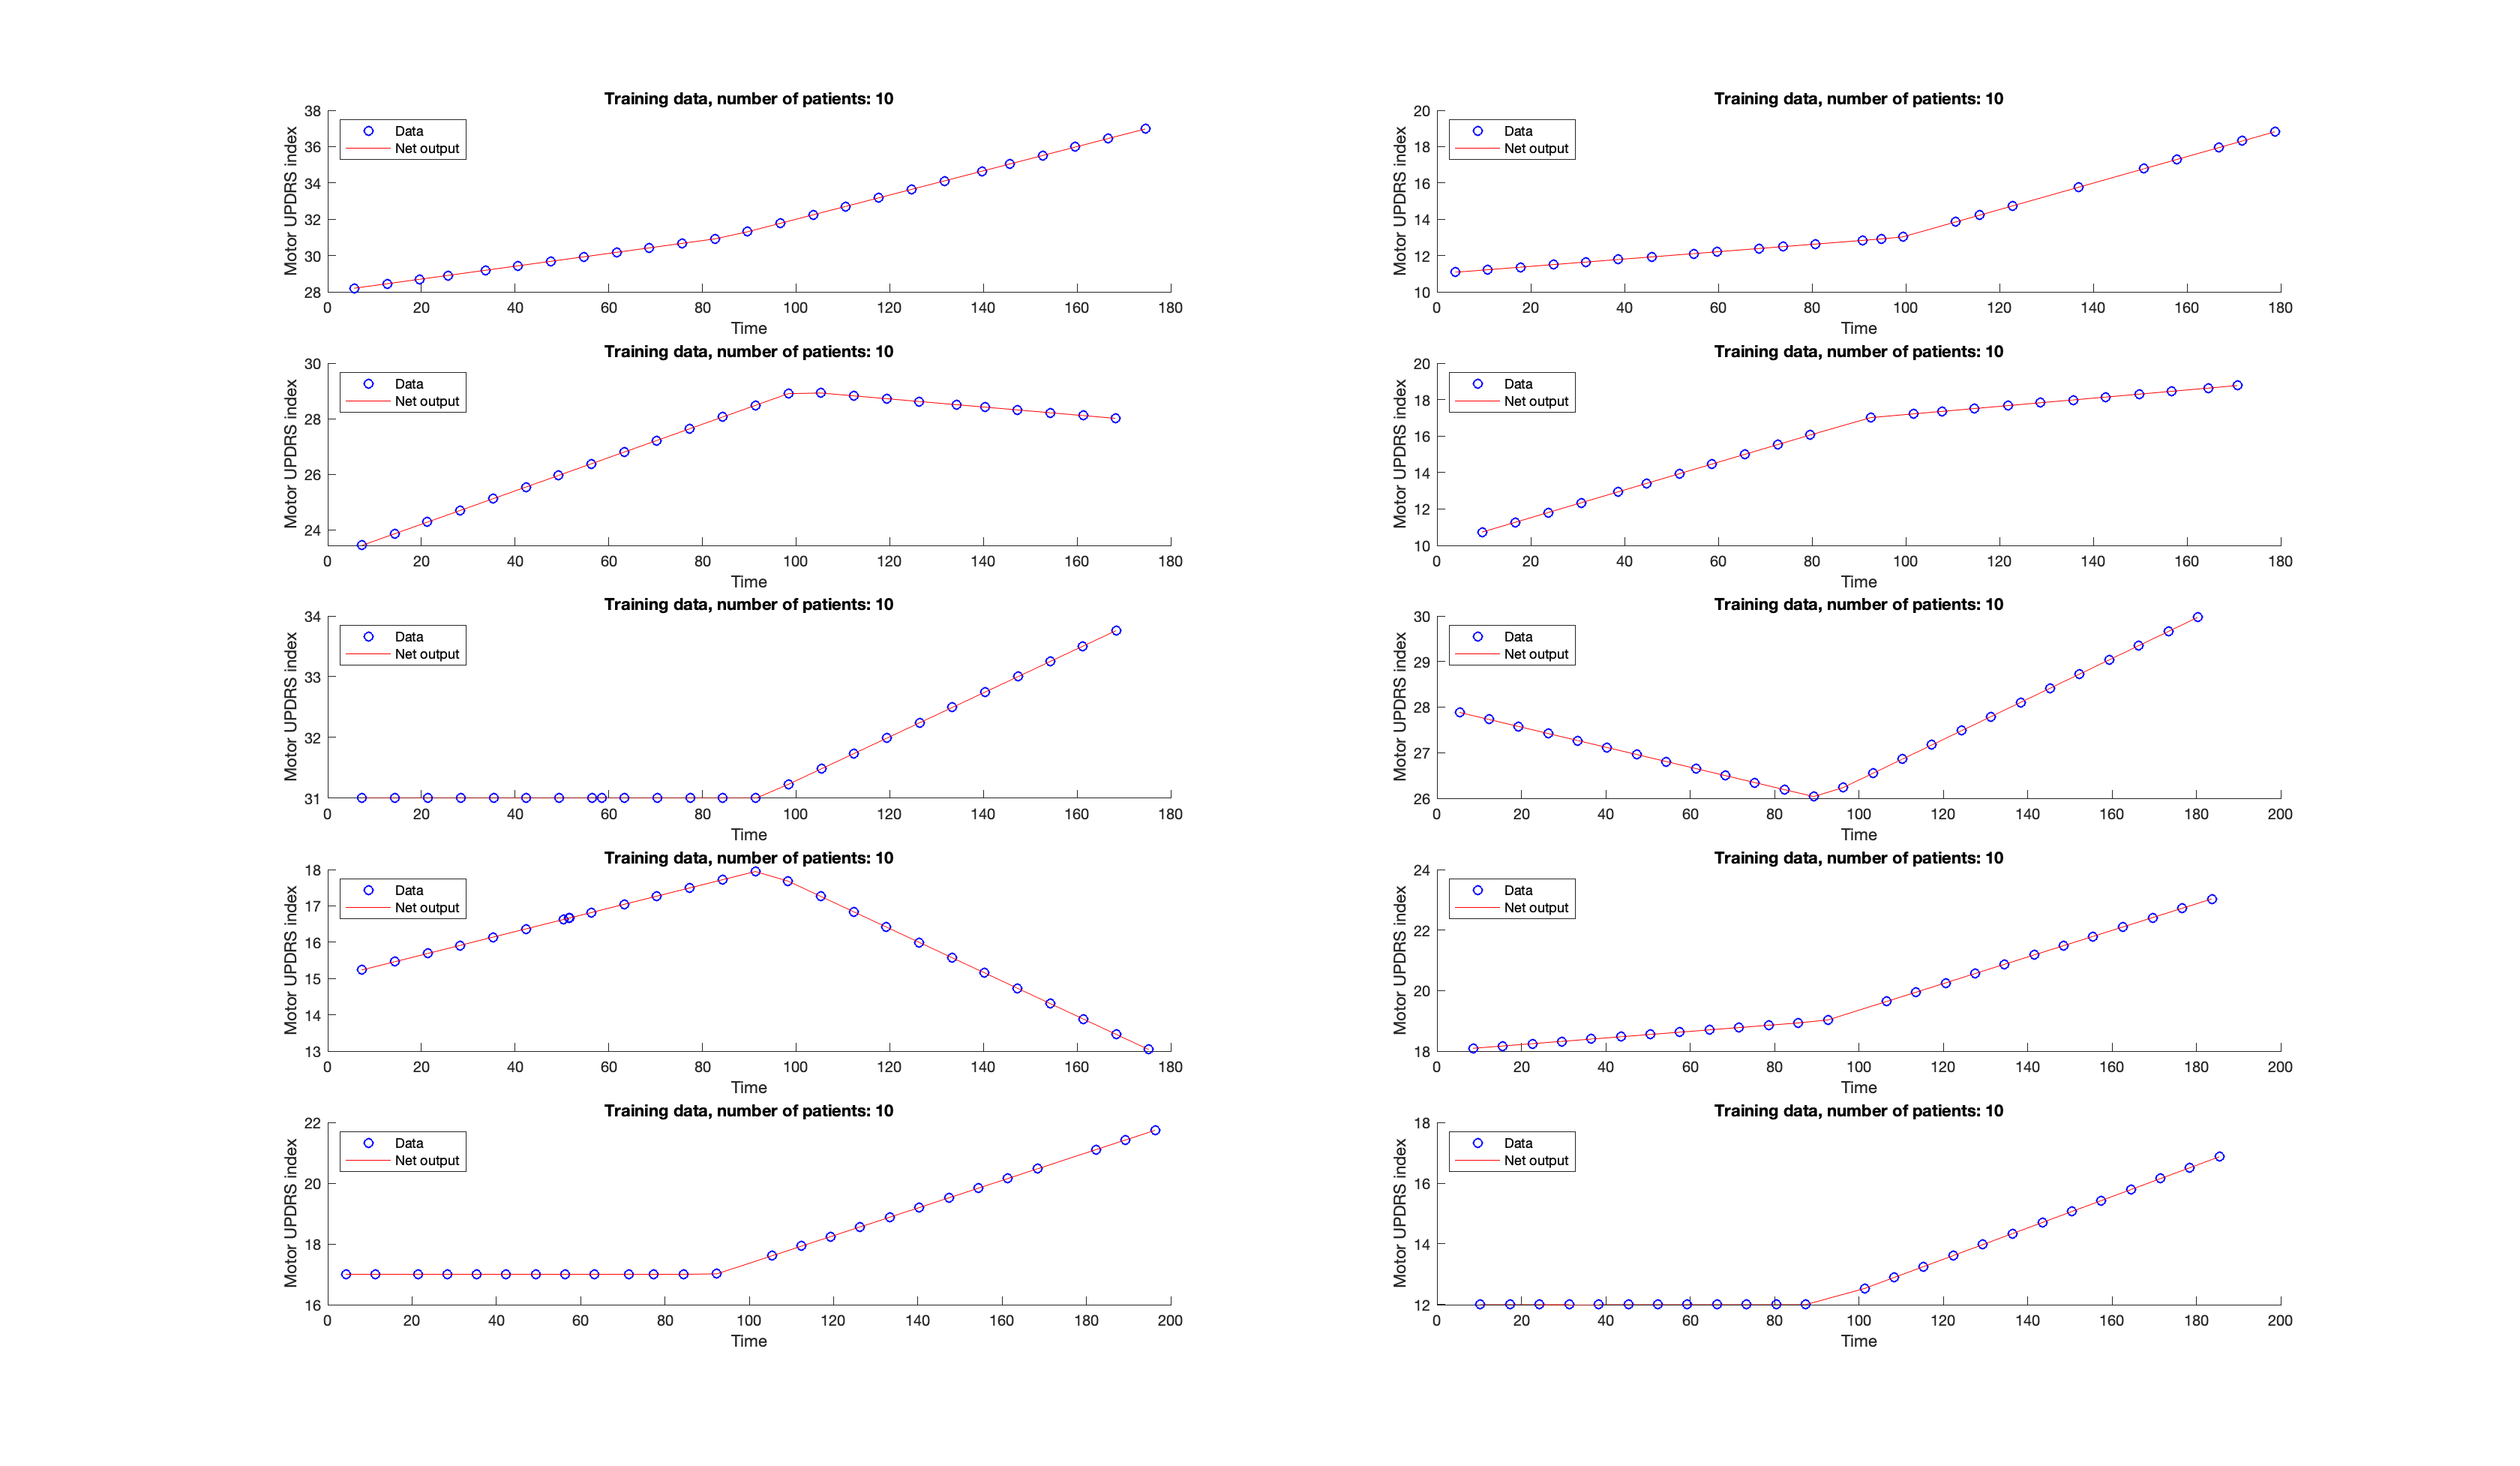
\includegraphics[width=1.05\textwidth]{training-cut-10.png}
\caption{Zbiór treningowy, 10 pacjentów}

\end{figure}

\begin{figure}[h!]

\centering
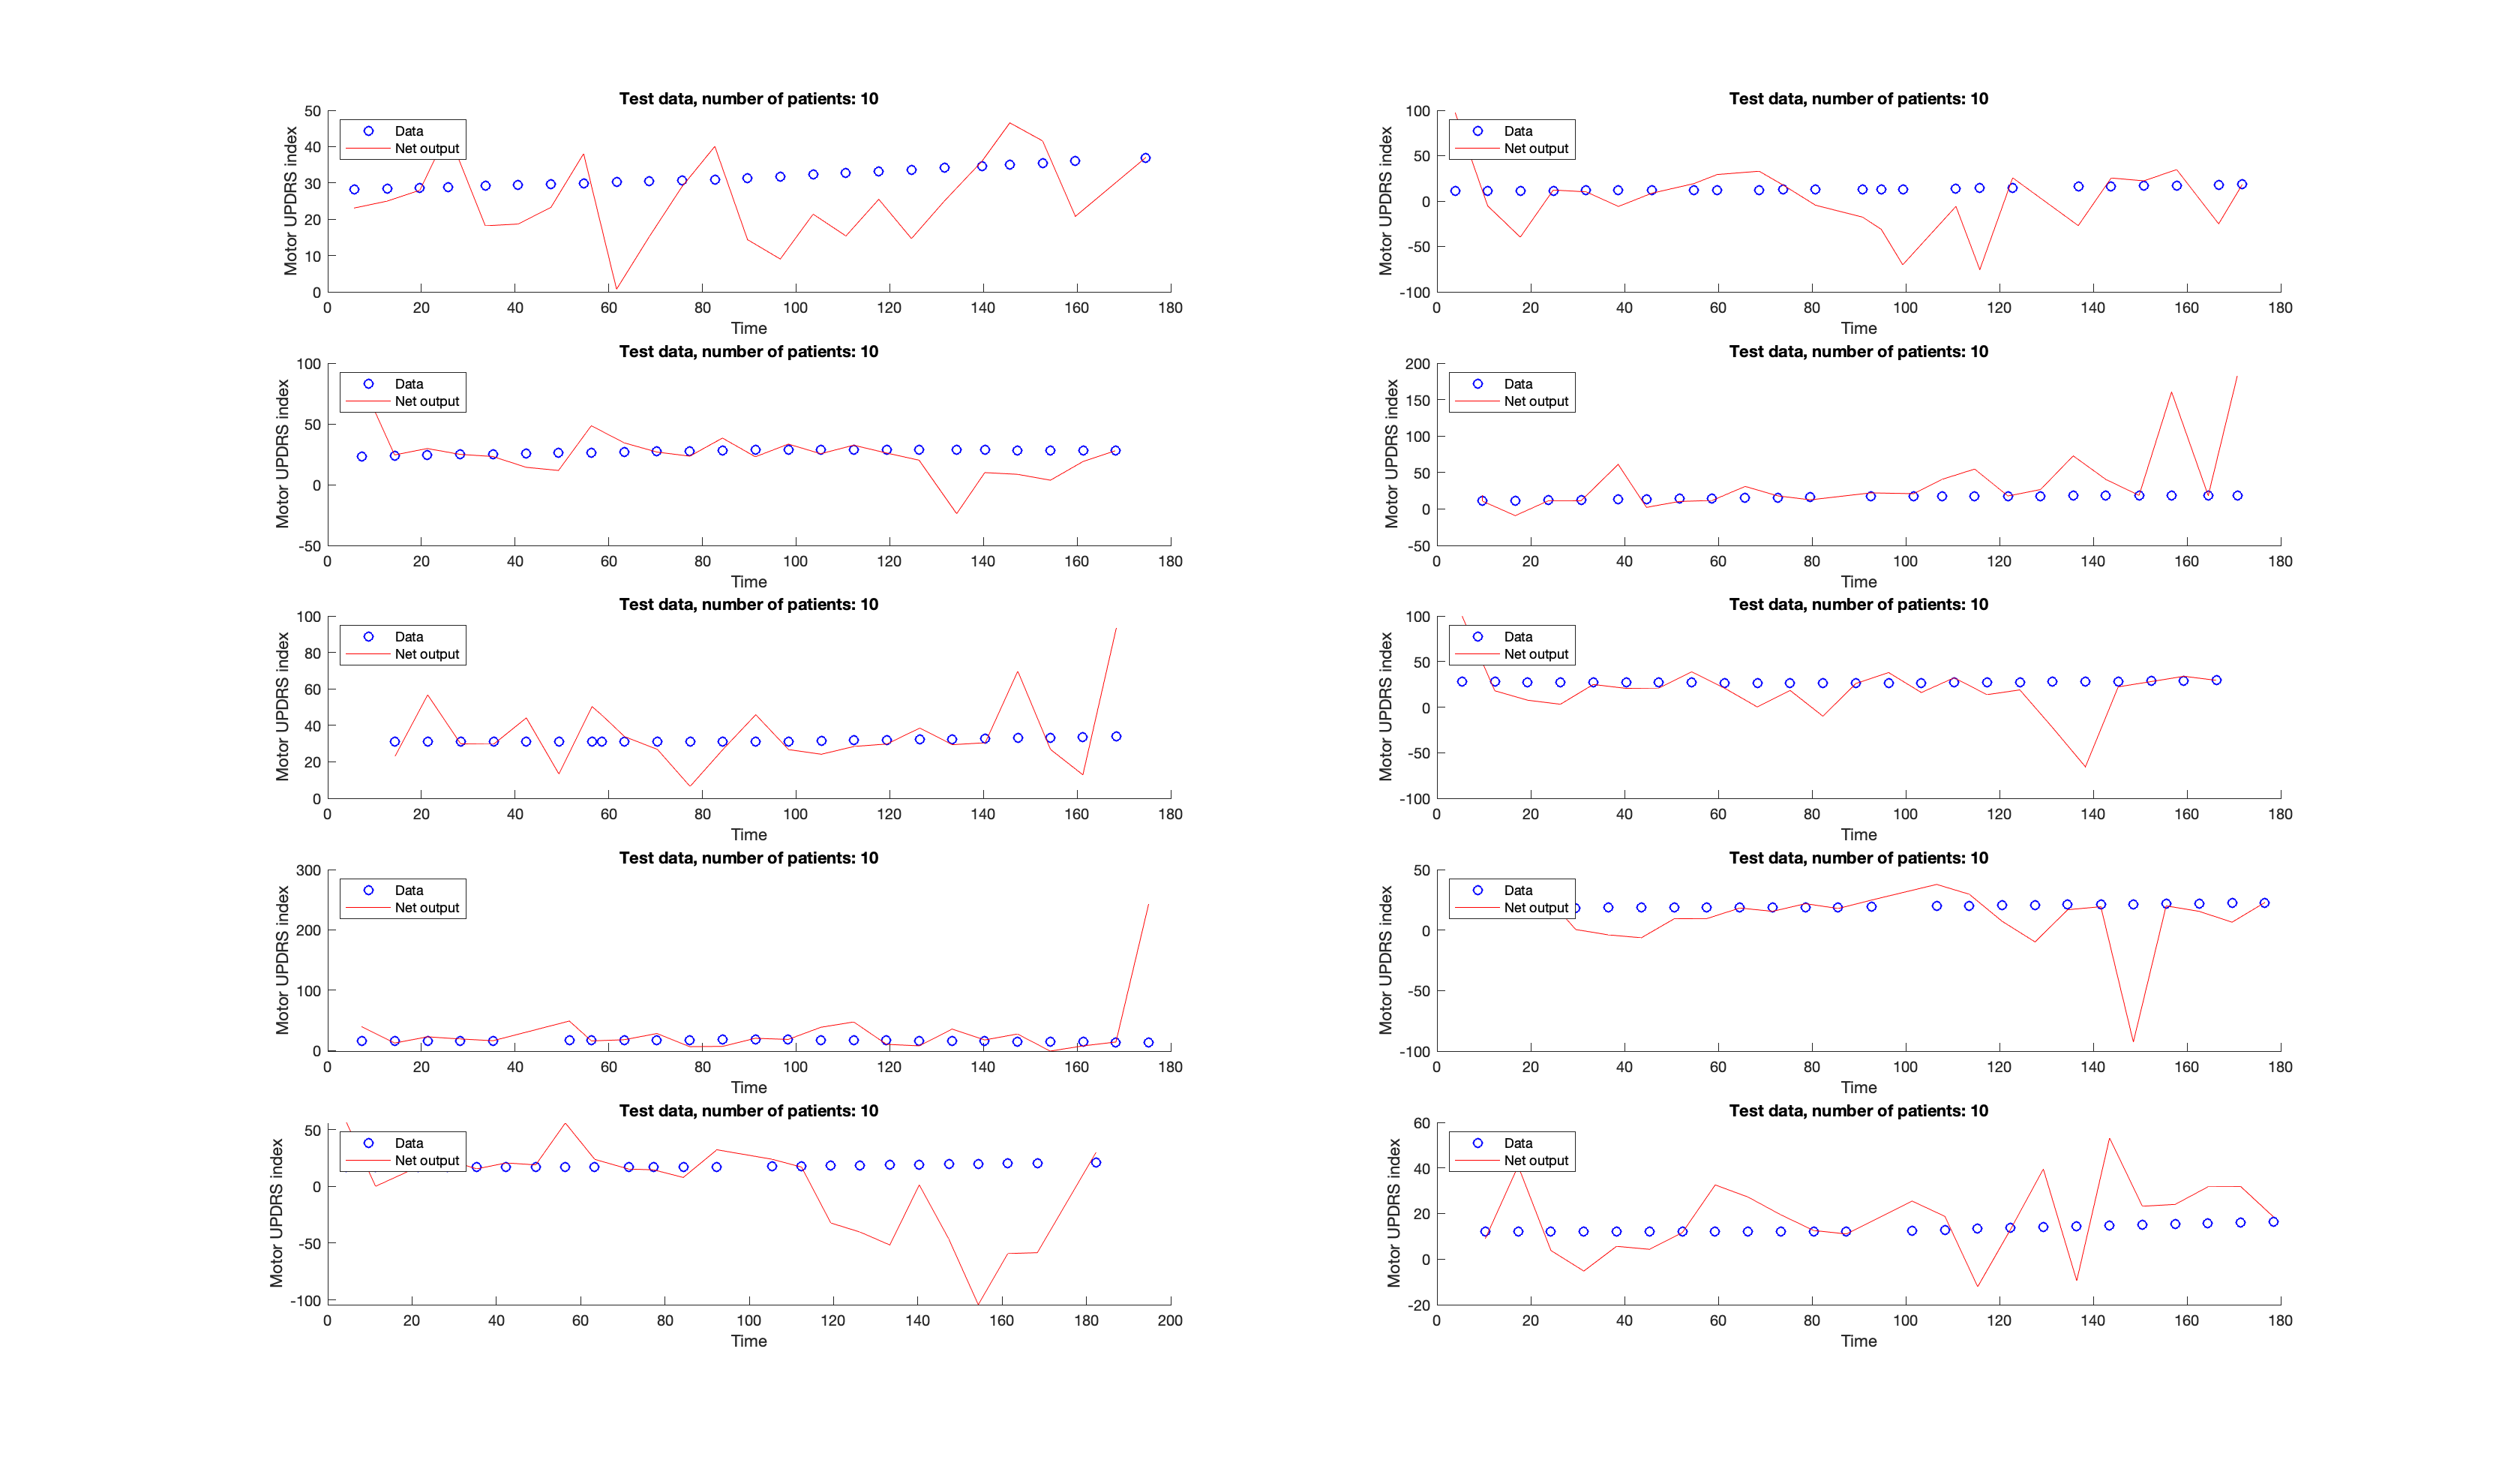
\includegraphics[width=1.0\textwidth]{test-cut-10.png}
\caption{Zbiór testowy, 10 pacjentów}

\end{figure}

\begin{figure}[h!]

\centering
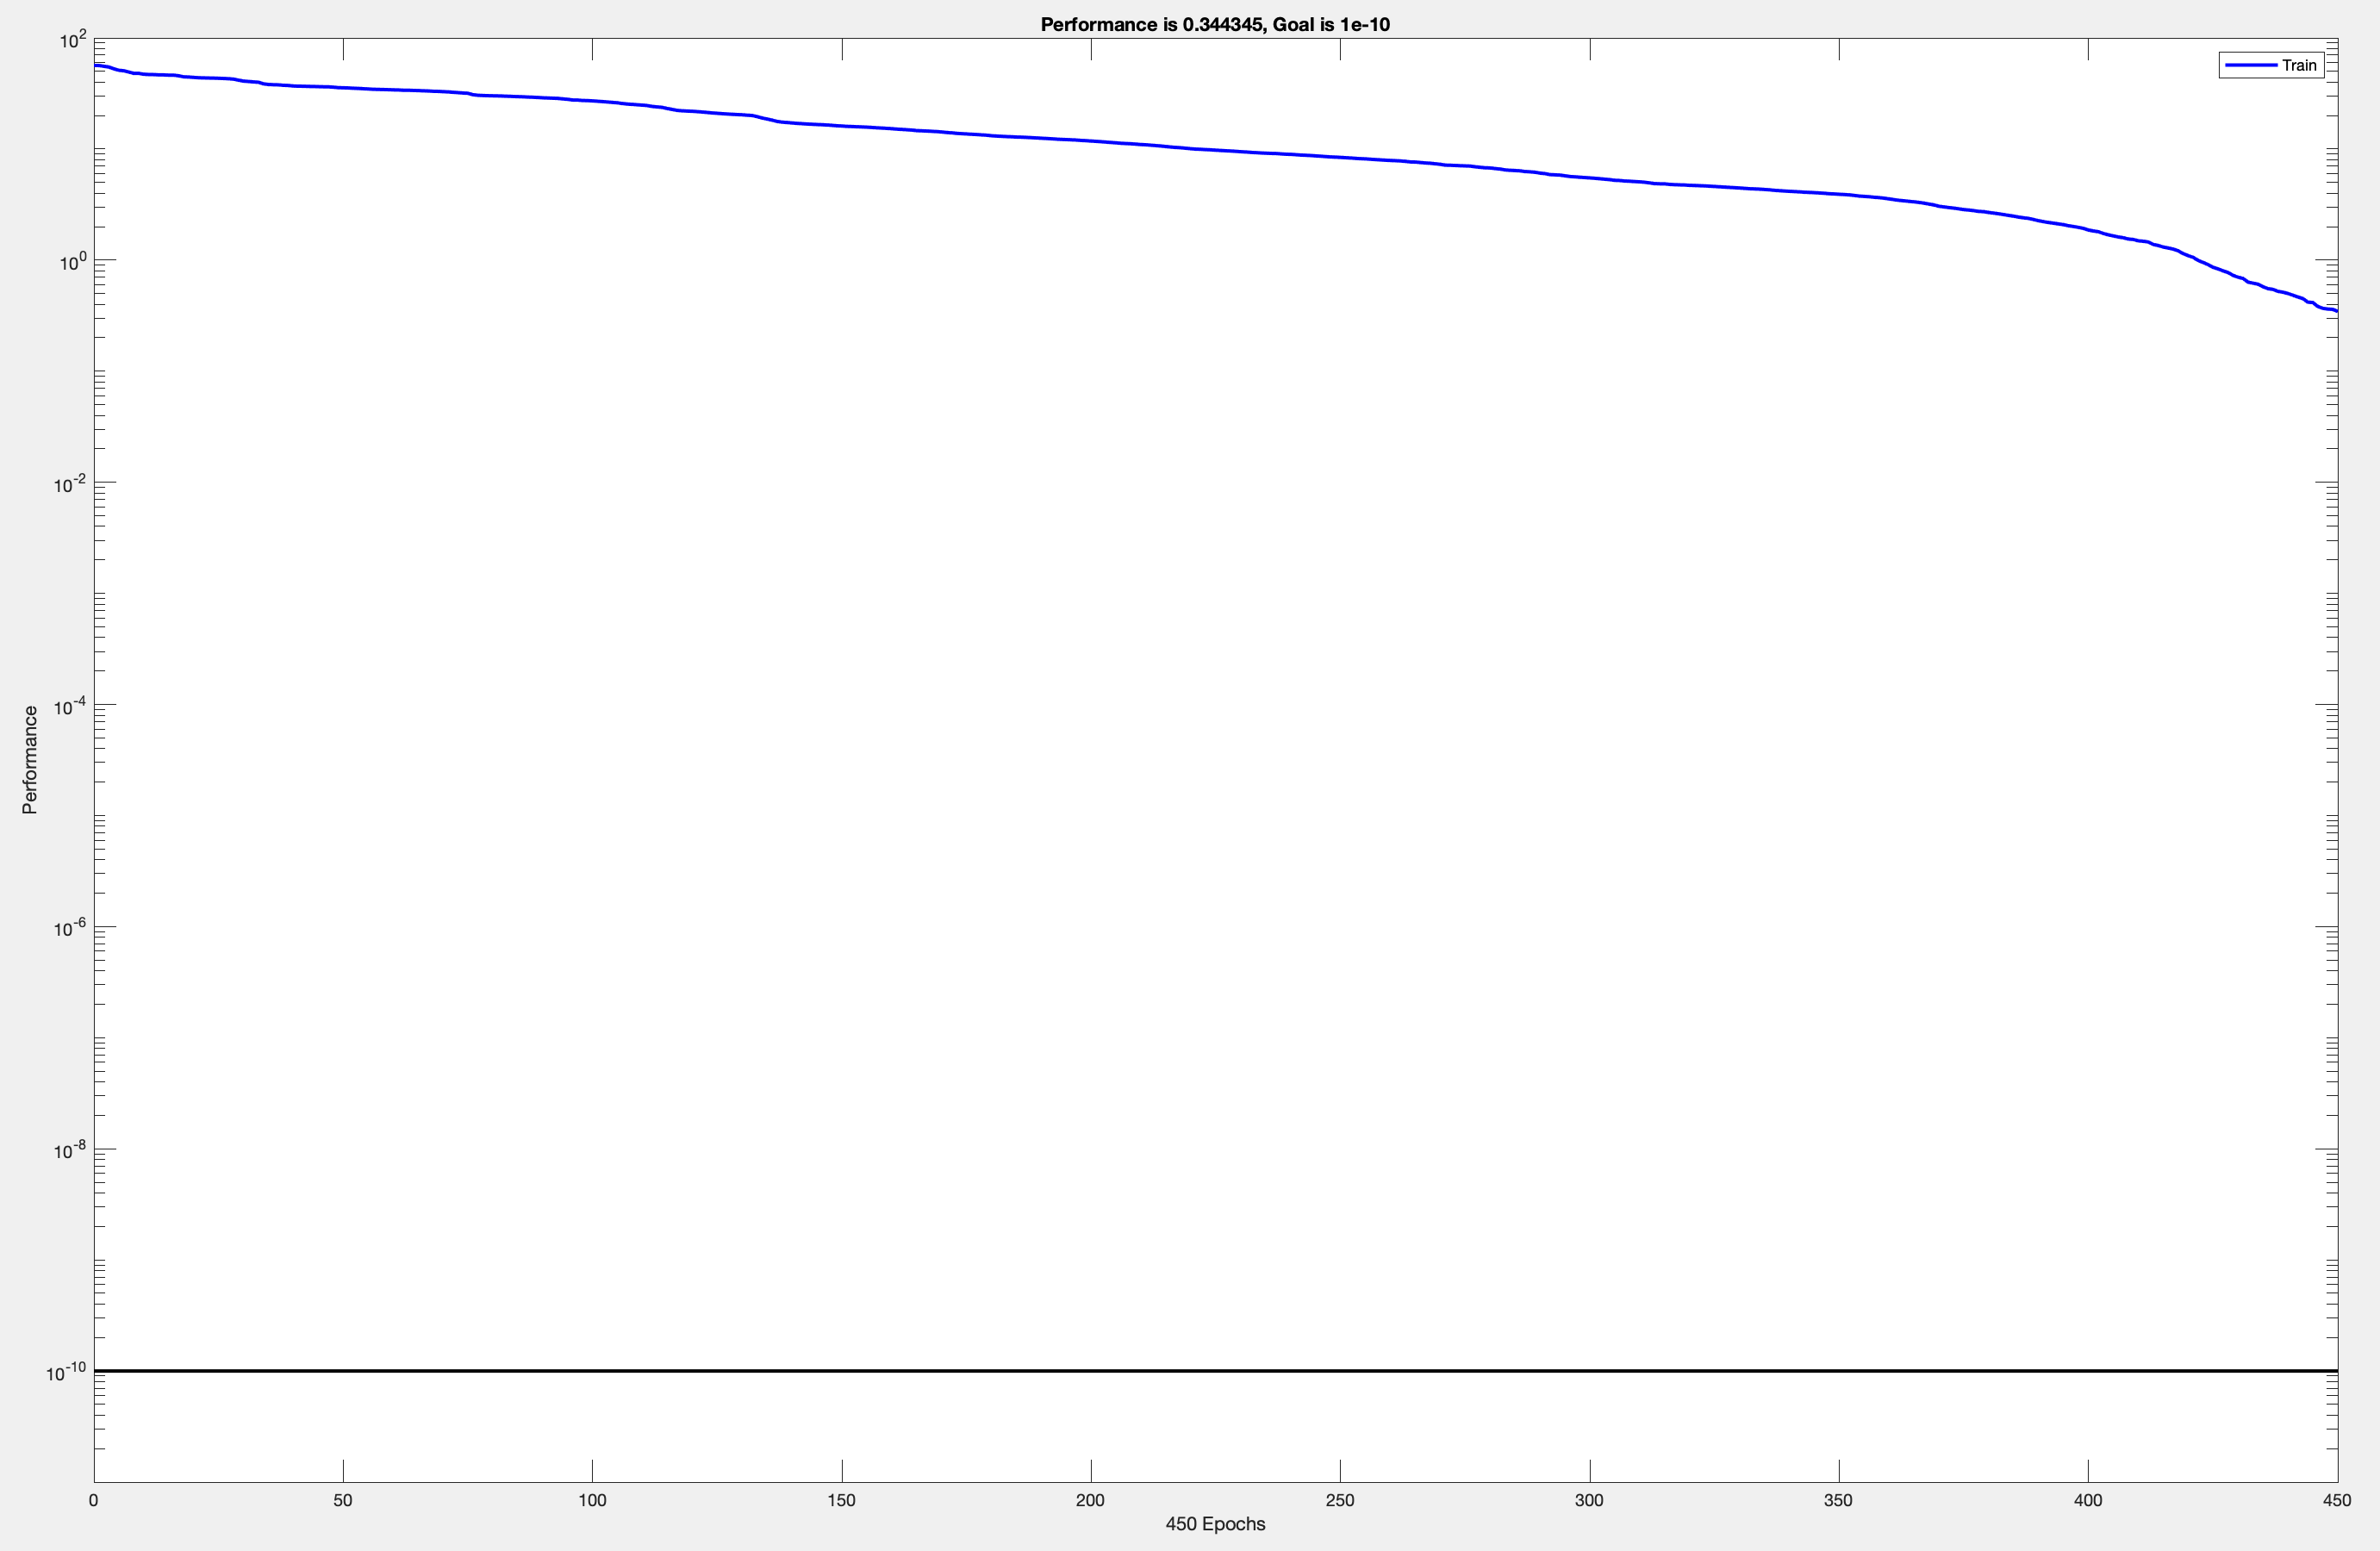
\includegraphics[width=0.9\textwidth]{mse-cut-20.png}
\caption{MSE dla 20 pacjentów}

\end{figure}

\begin{figure}[h!]

\centering
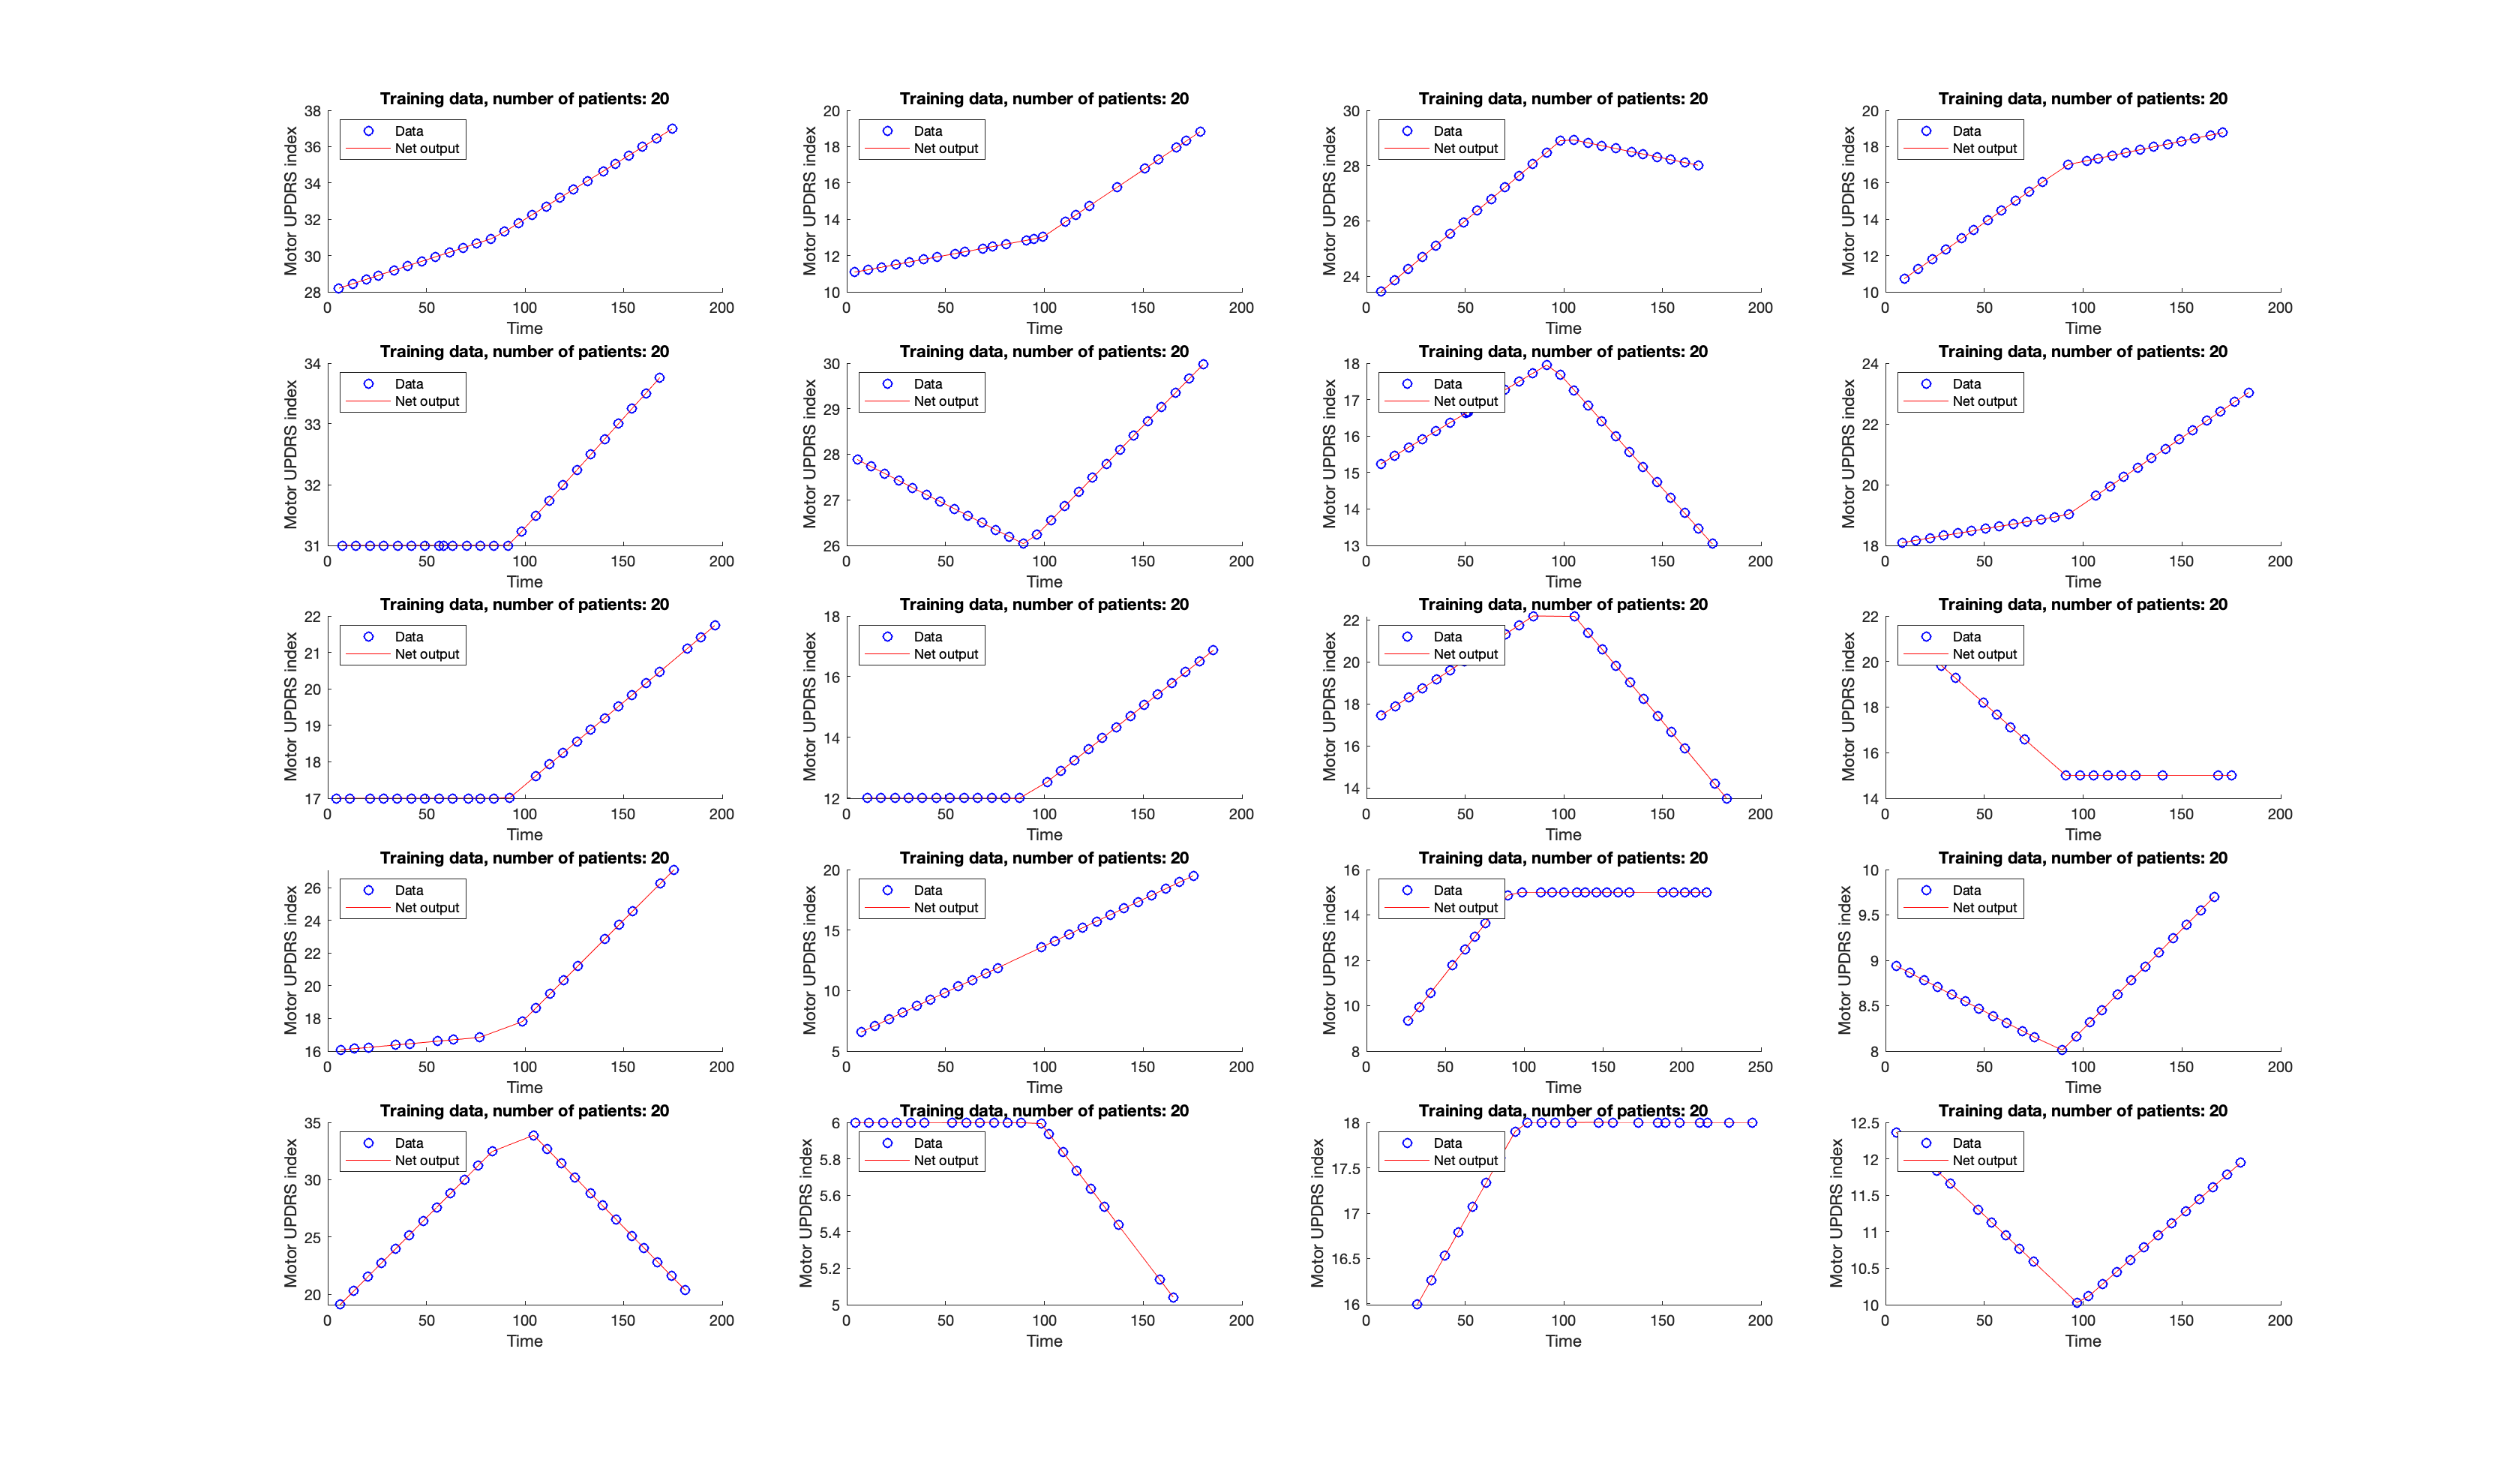
\includegraphics[width=1.0\textwidth]{training-cut-20.png}
\caption{Zbiór treningowy, 20 pacjentów}

\end{figure}

\begin{figure}[h!]

\centering
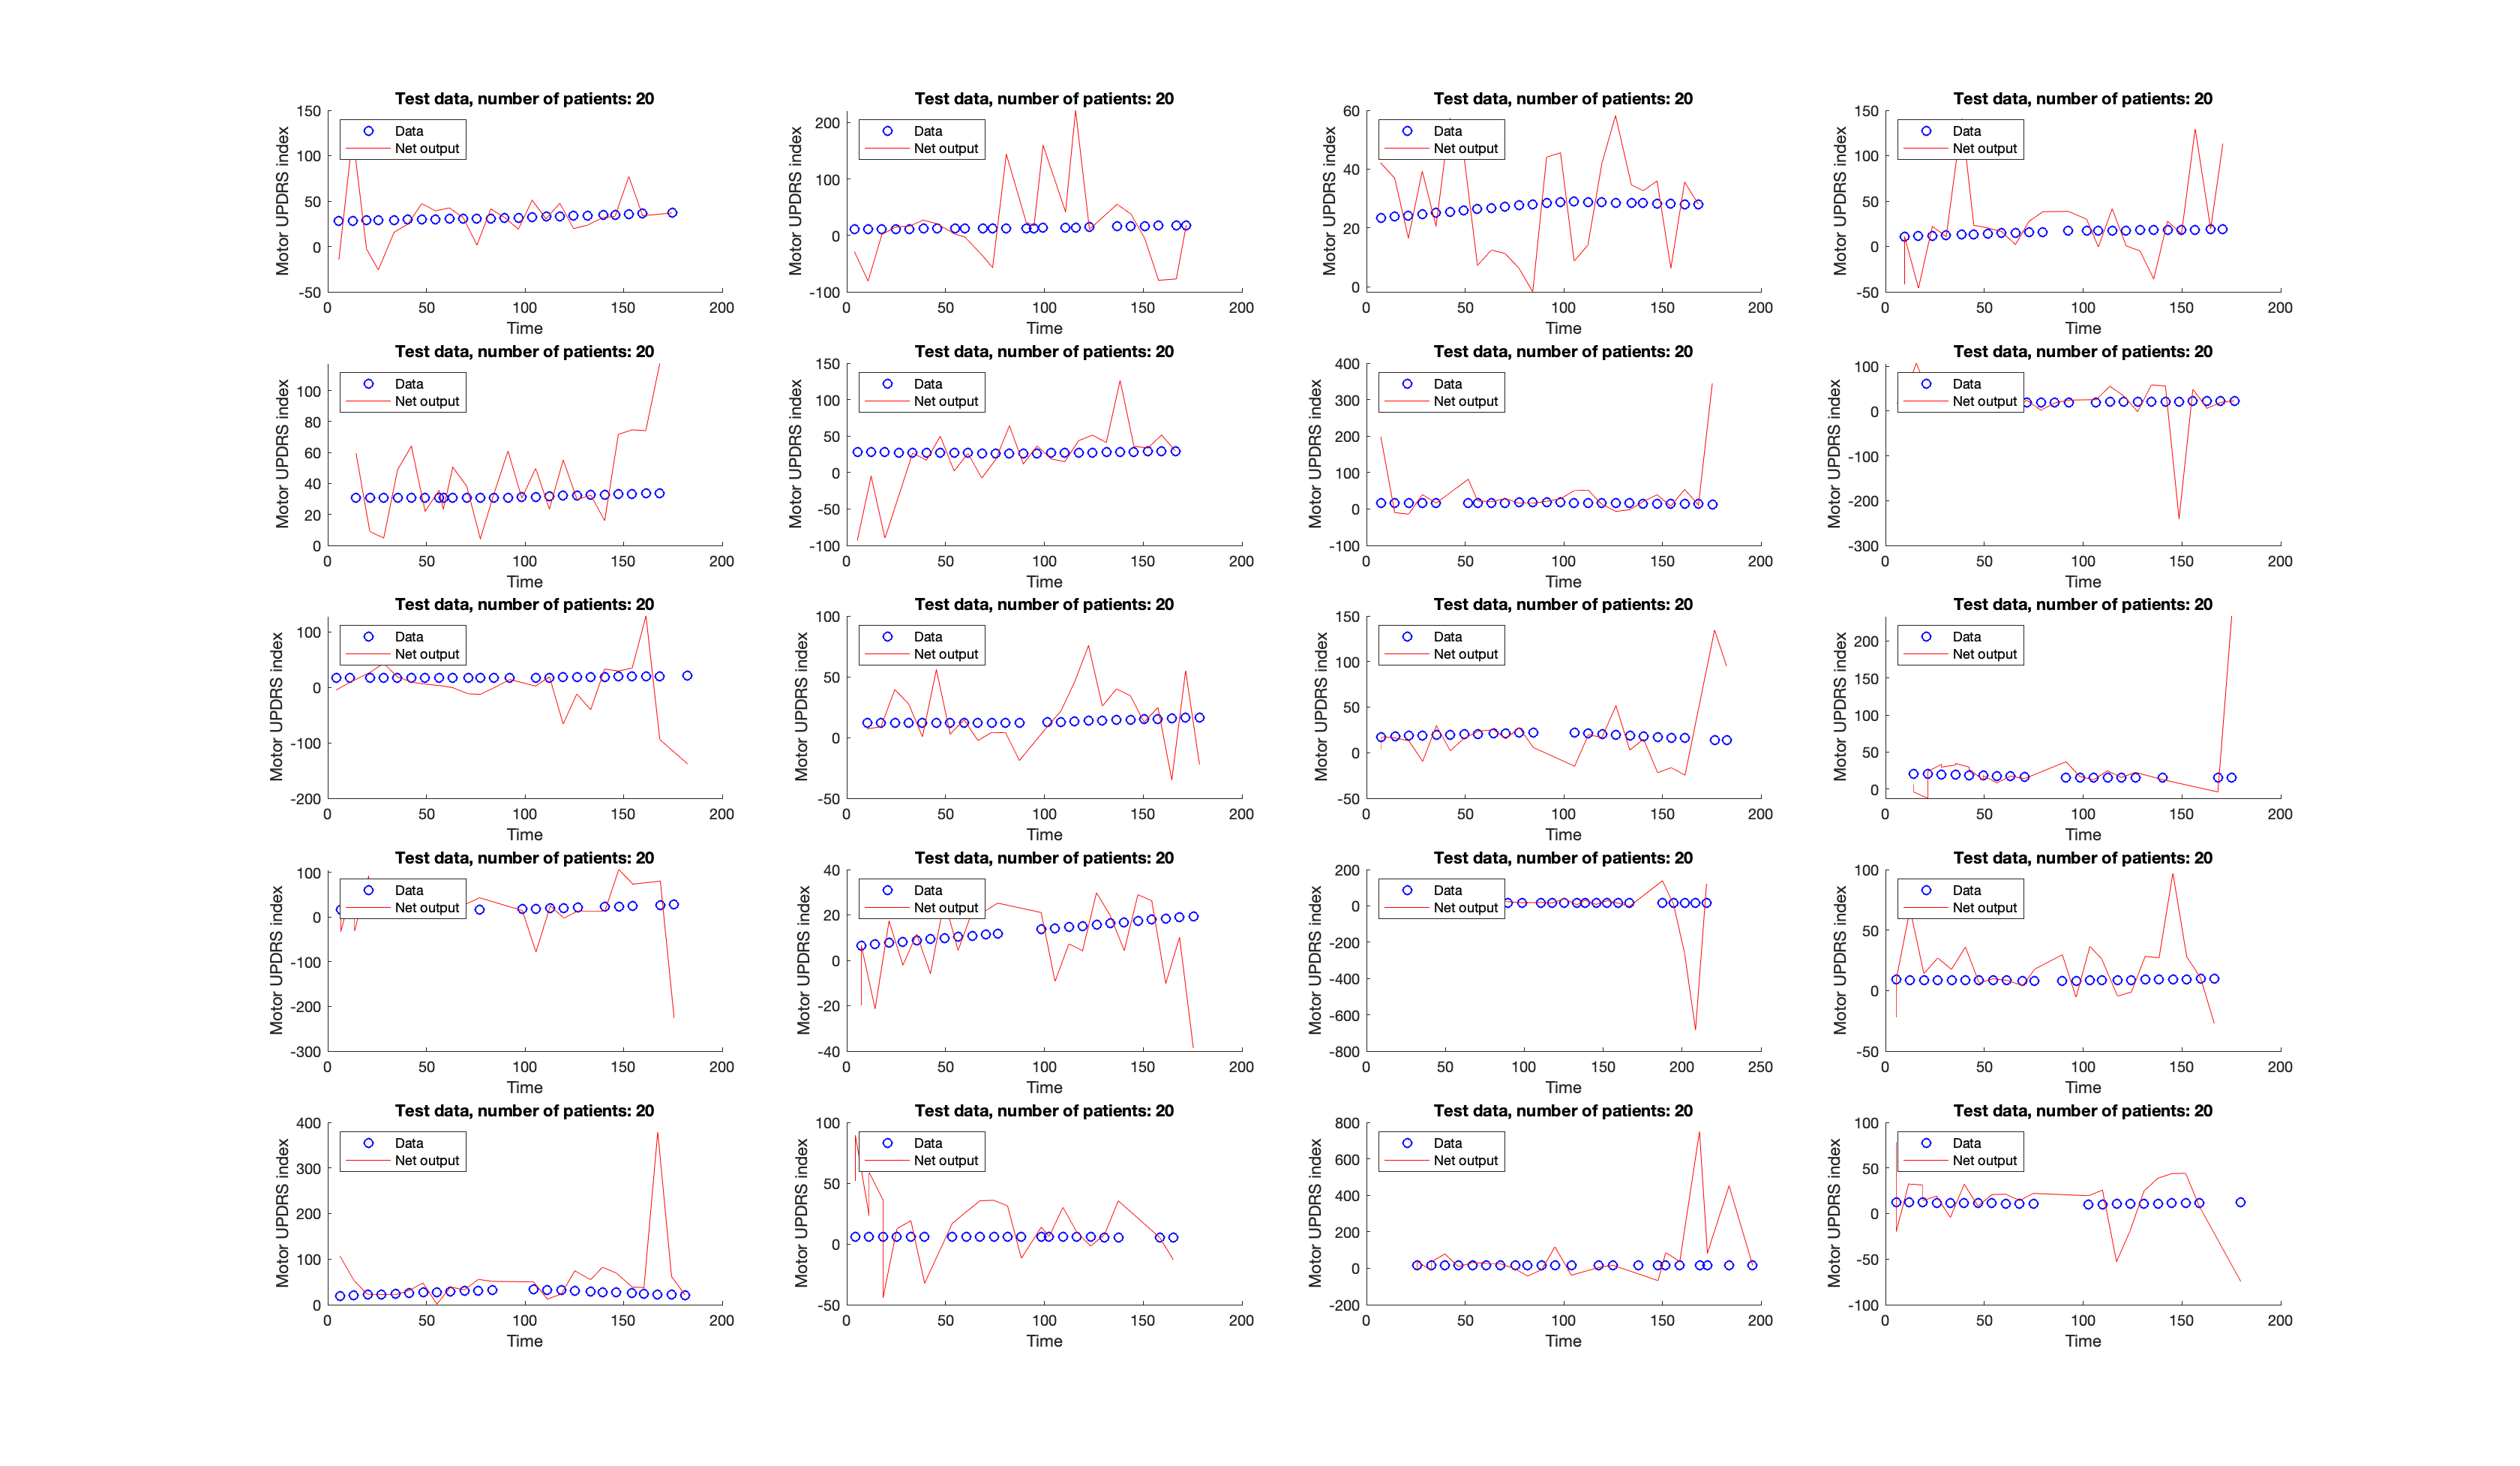
\includegraphics[width=1.1\textwidth]{test-cut-20.png}
\caption{Zbiór testowy, 20 pacjentów}

\end{figure}

\newpage

Dla małej ilości pacjentów oraz zbioru uczącego nie zawierającego duplikatów sieć wykazuje dopasowanie, choć widać błędy w predykcji pewnych klas pacjentów. Mała ilość danych uczących znacząco przyspiesza naukę, co pozwala na wykonanie predykcji w przypadku większej liczby pacjentów.

\subsection{Dane bez duplikatów próbek czasowych z dużą ilością pacjentów}

Parametry uczenia:
\begin{itemize}
\item Mean squared error: $10^{-9}$
\item Spread constant: $50$
\end{itemize}

\newpage

\begin{figure}[h!]

\centering
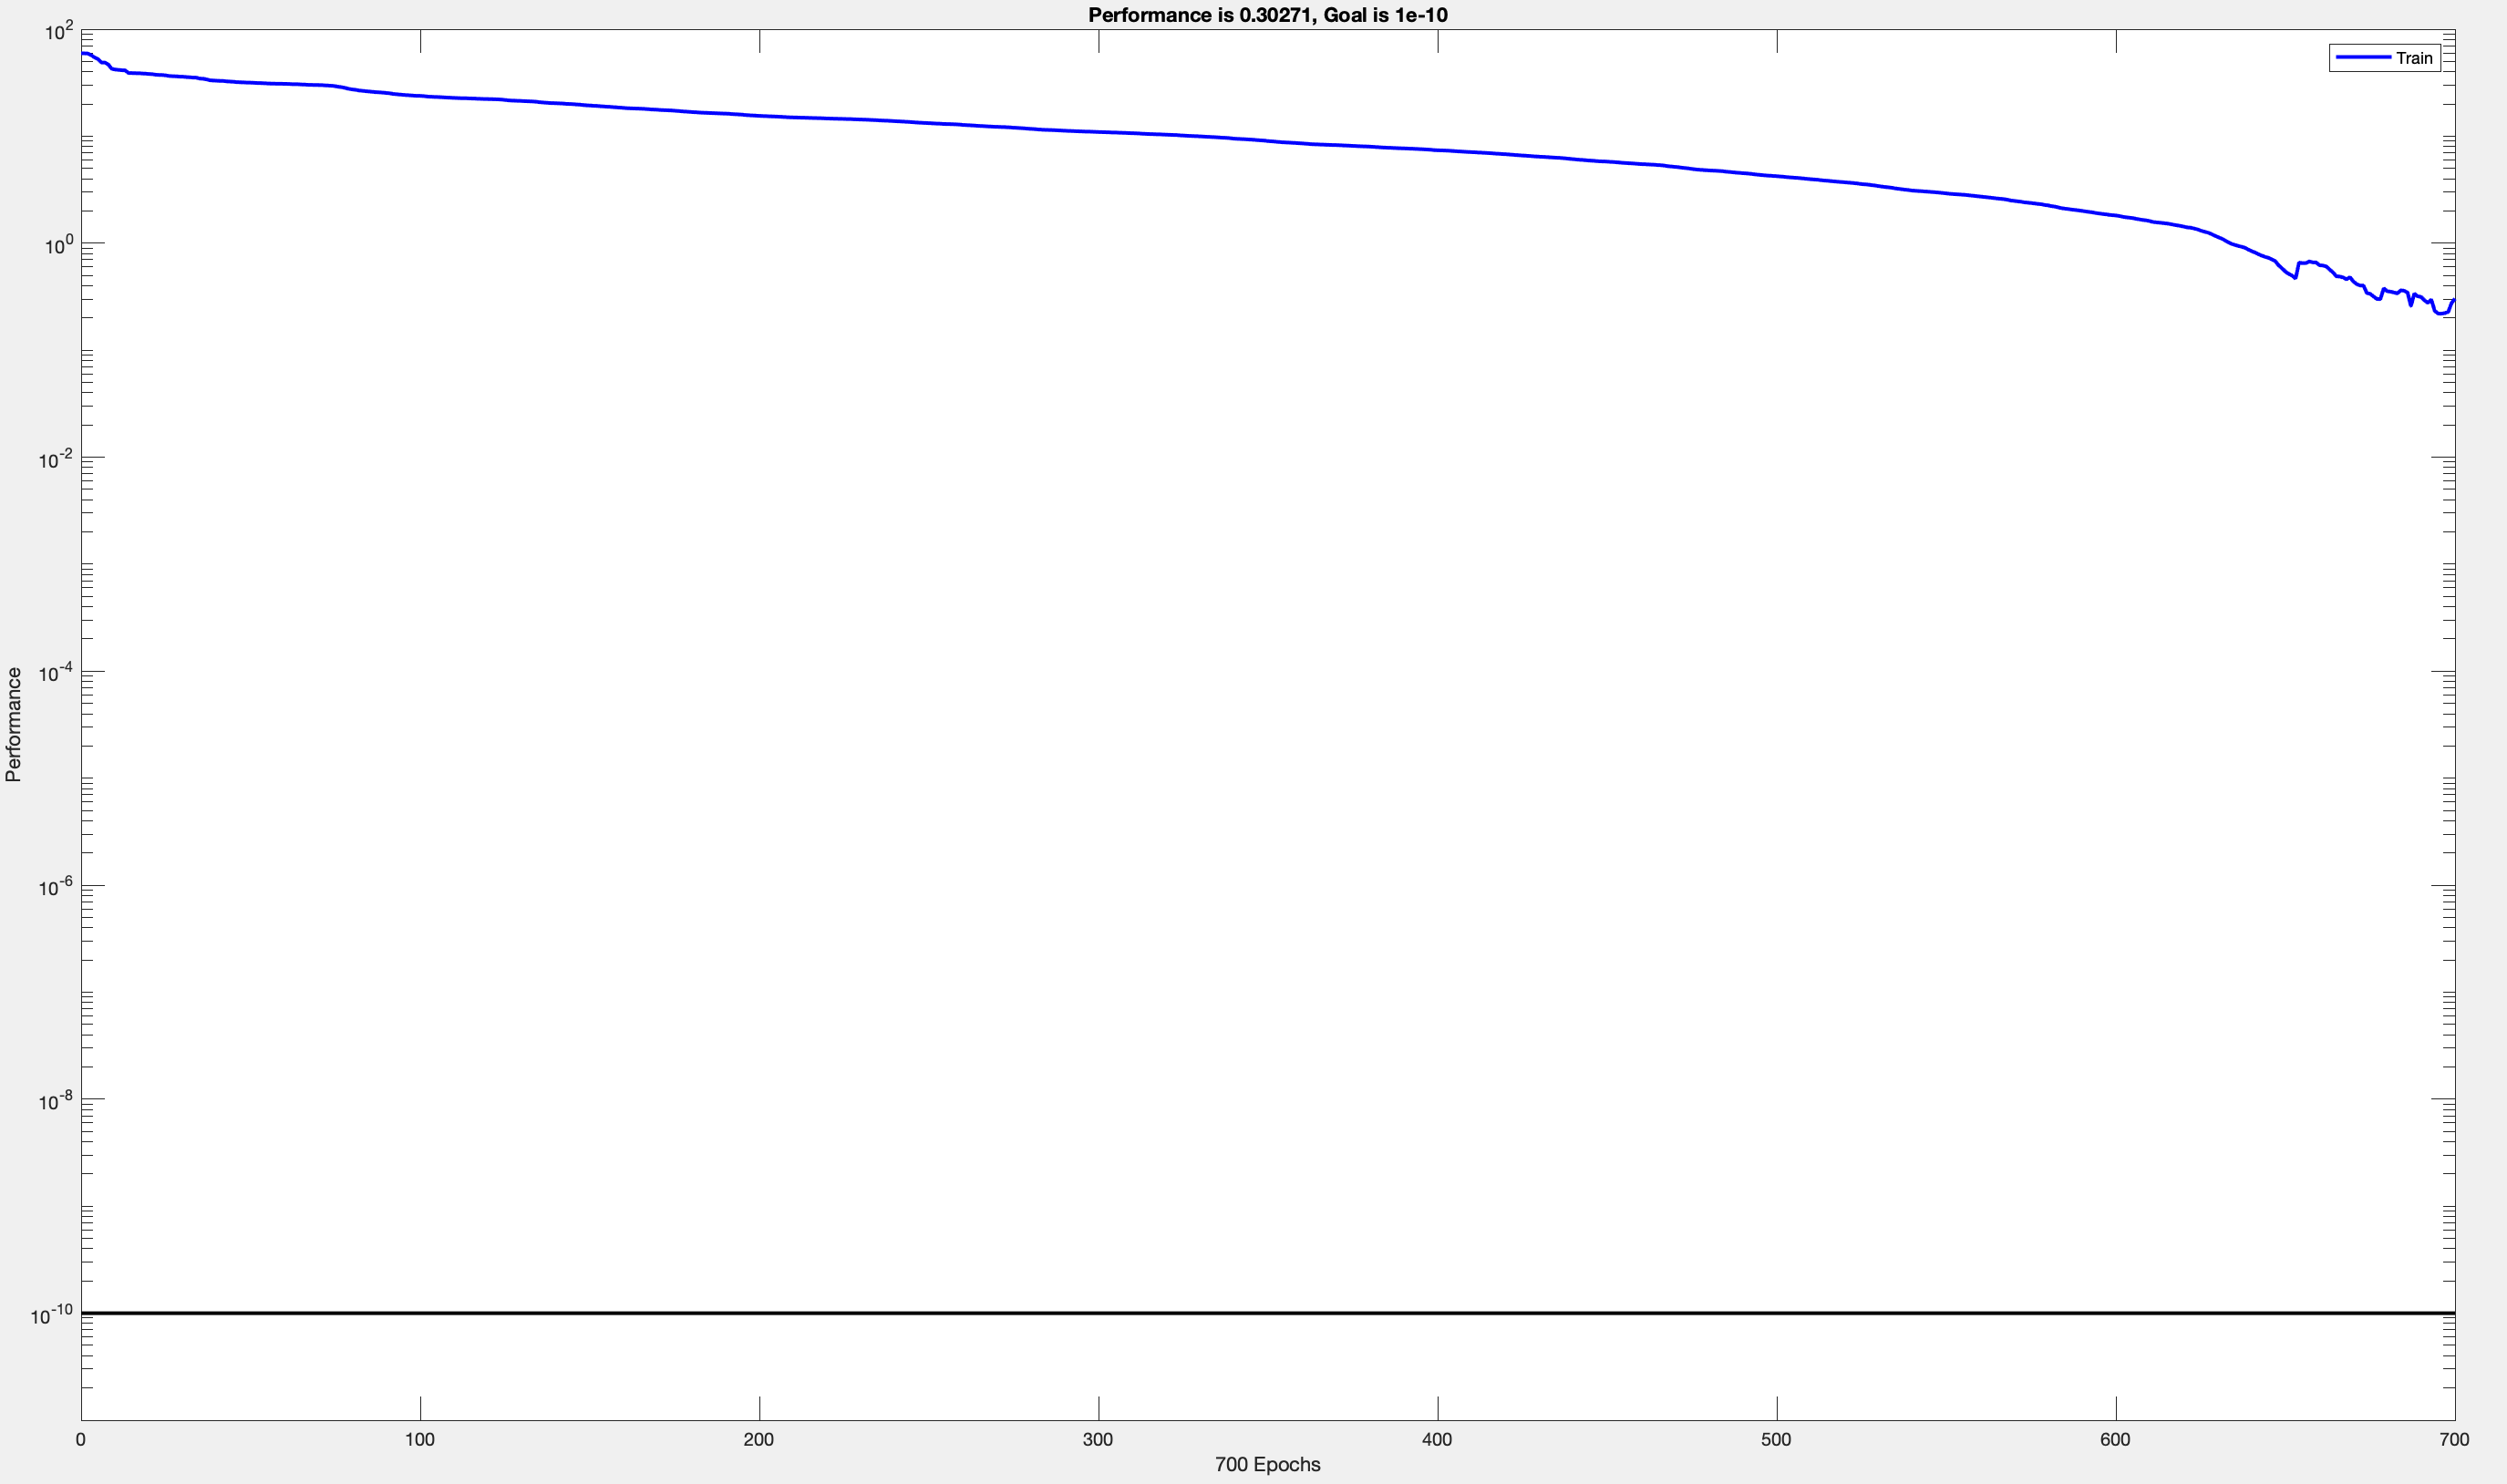
\includegraphics[width=0.9\textwidth]{mse-cut-30.png}
\caption{MSE dla 30 pacjentów}

\end{figure}

\begin{figure}[h!]

\centering
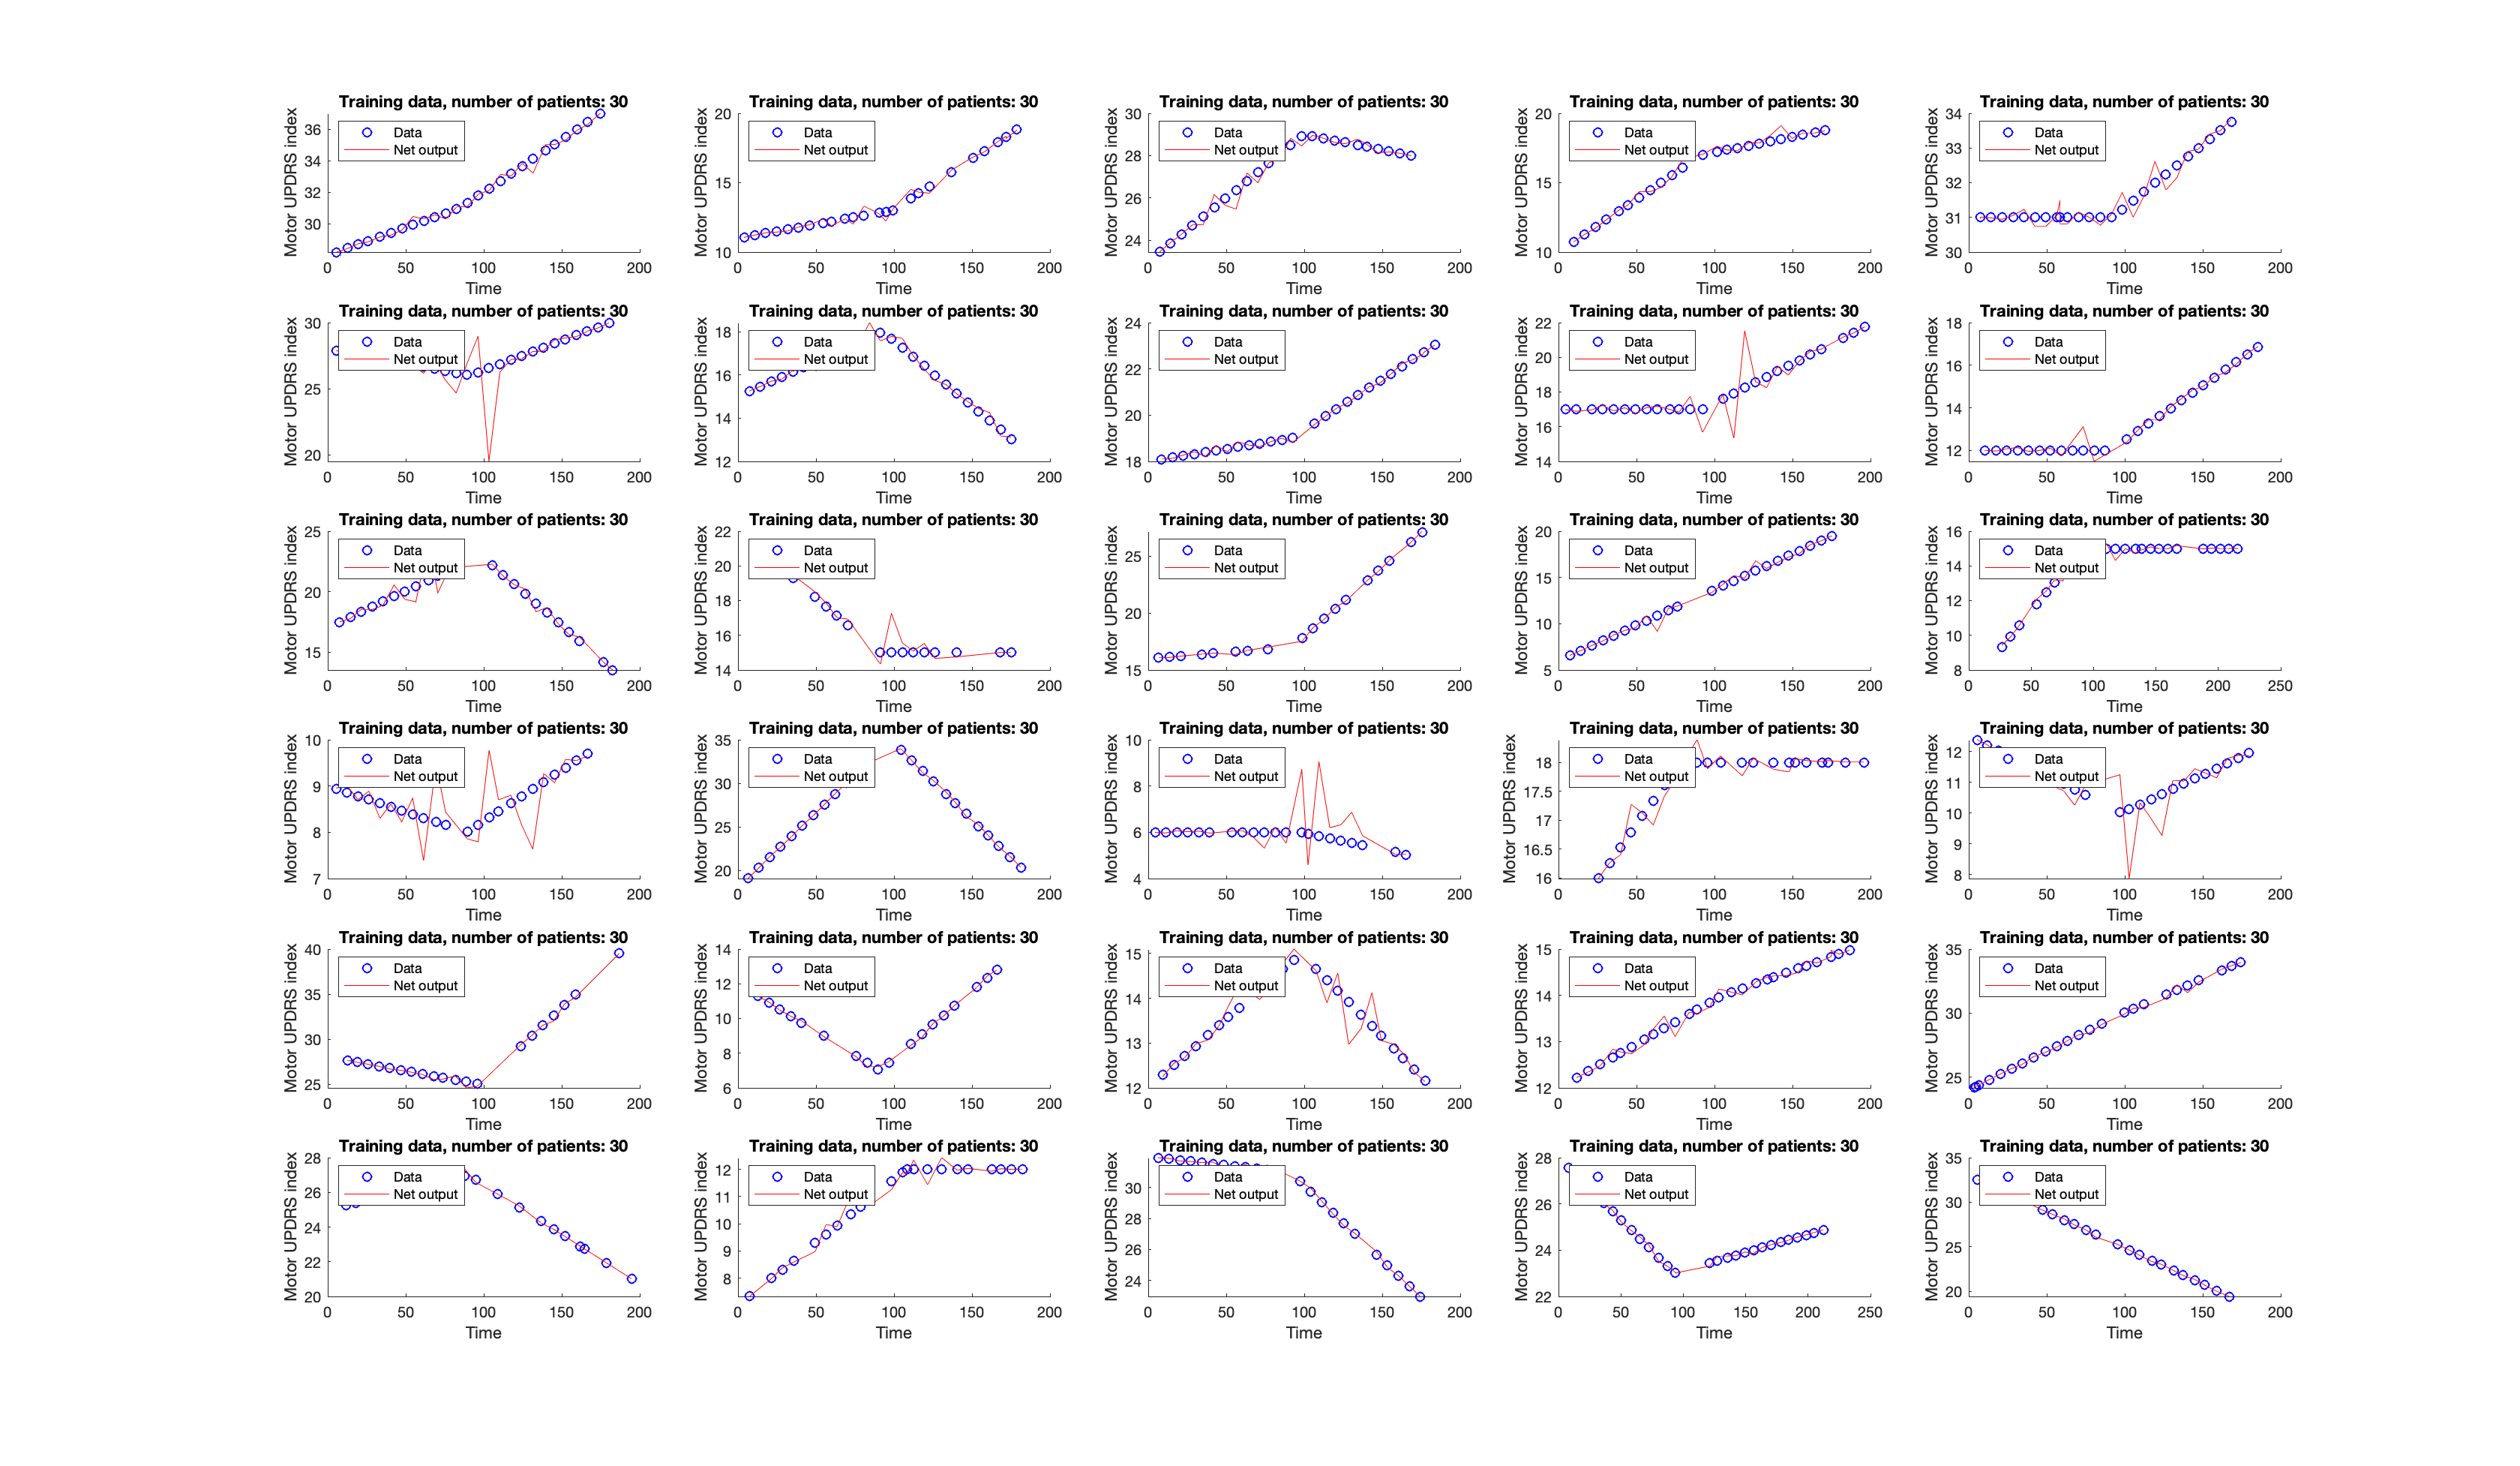
\includegraphics[width=1.05\textwidth]{training-cut-30.png}
\caption{Zbiór treningowy, 30 pacjentów}

\end{figure}

\begin{figure}[h!]

\centering
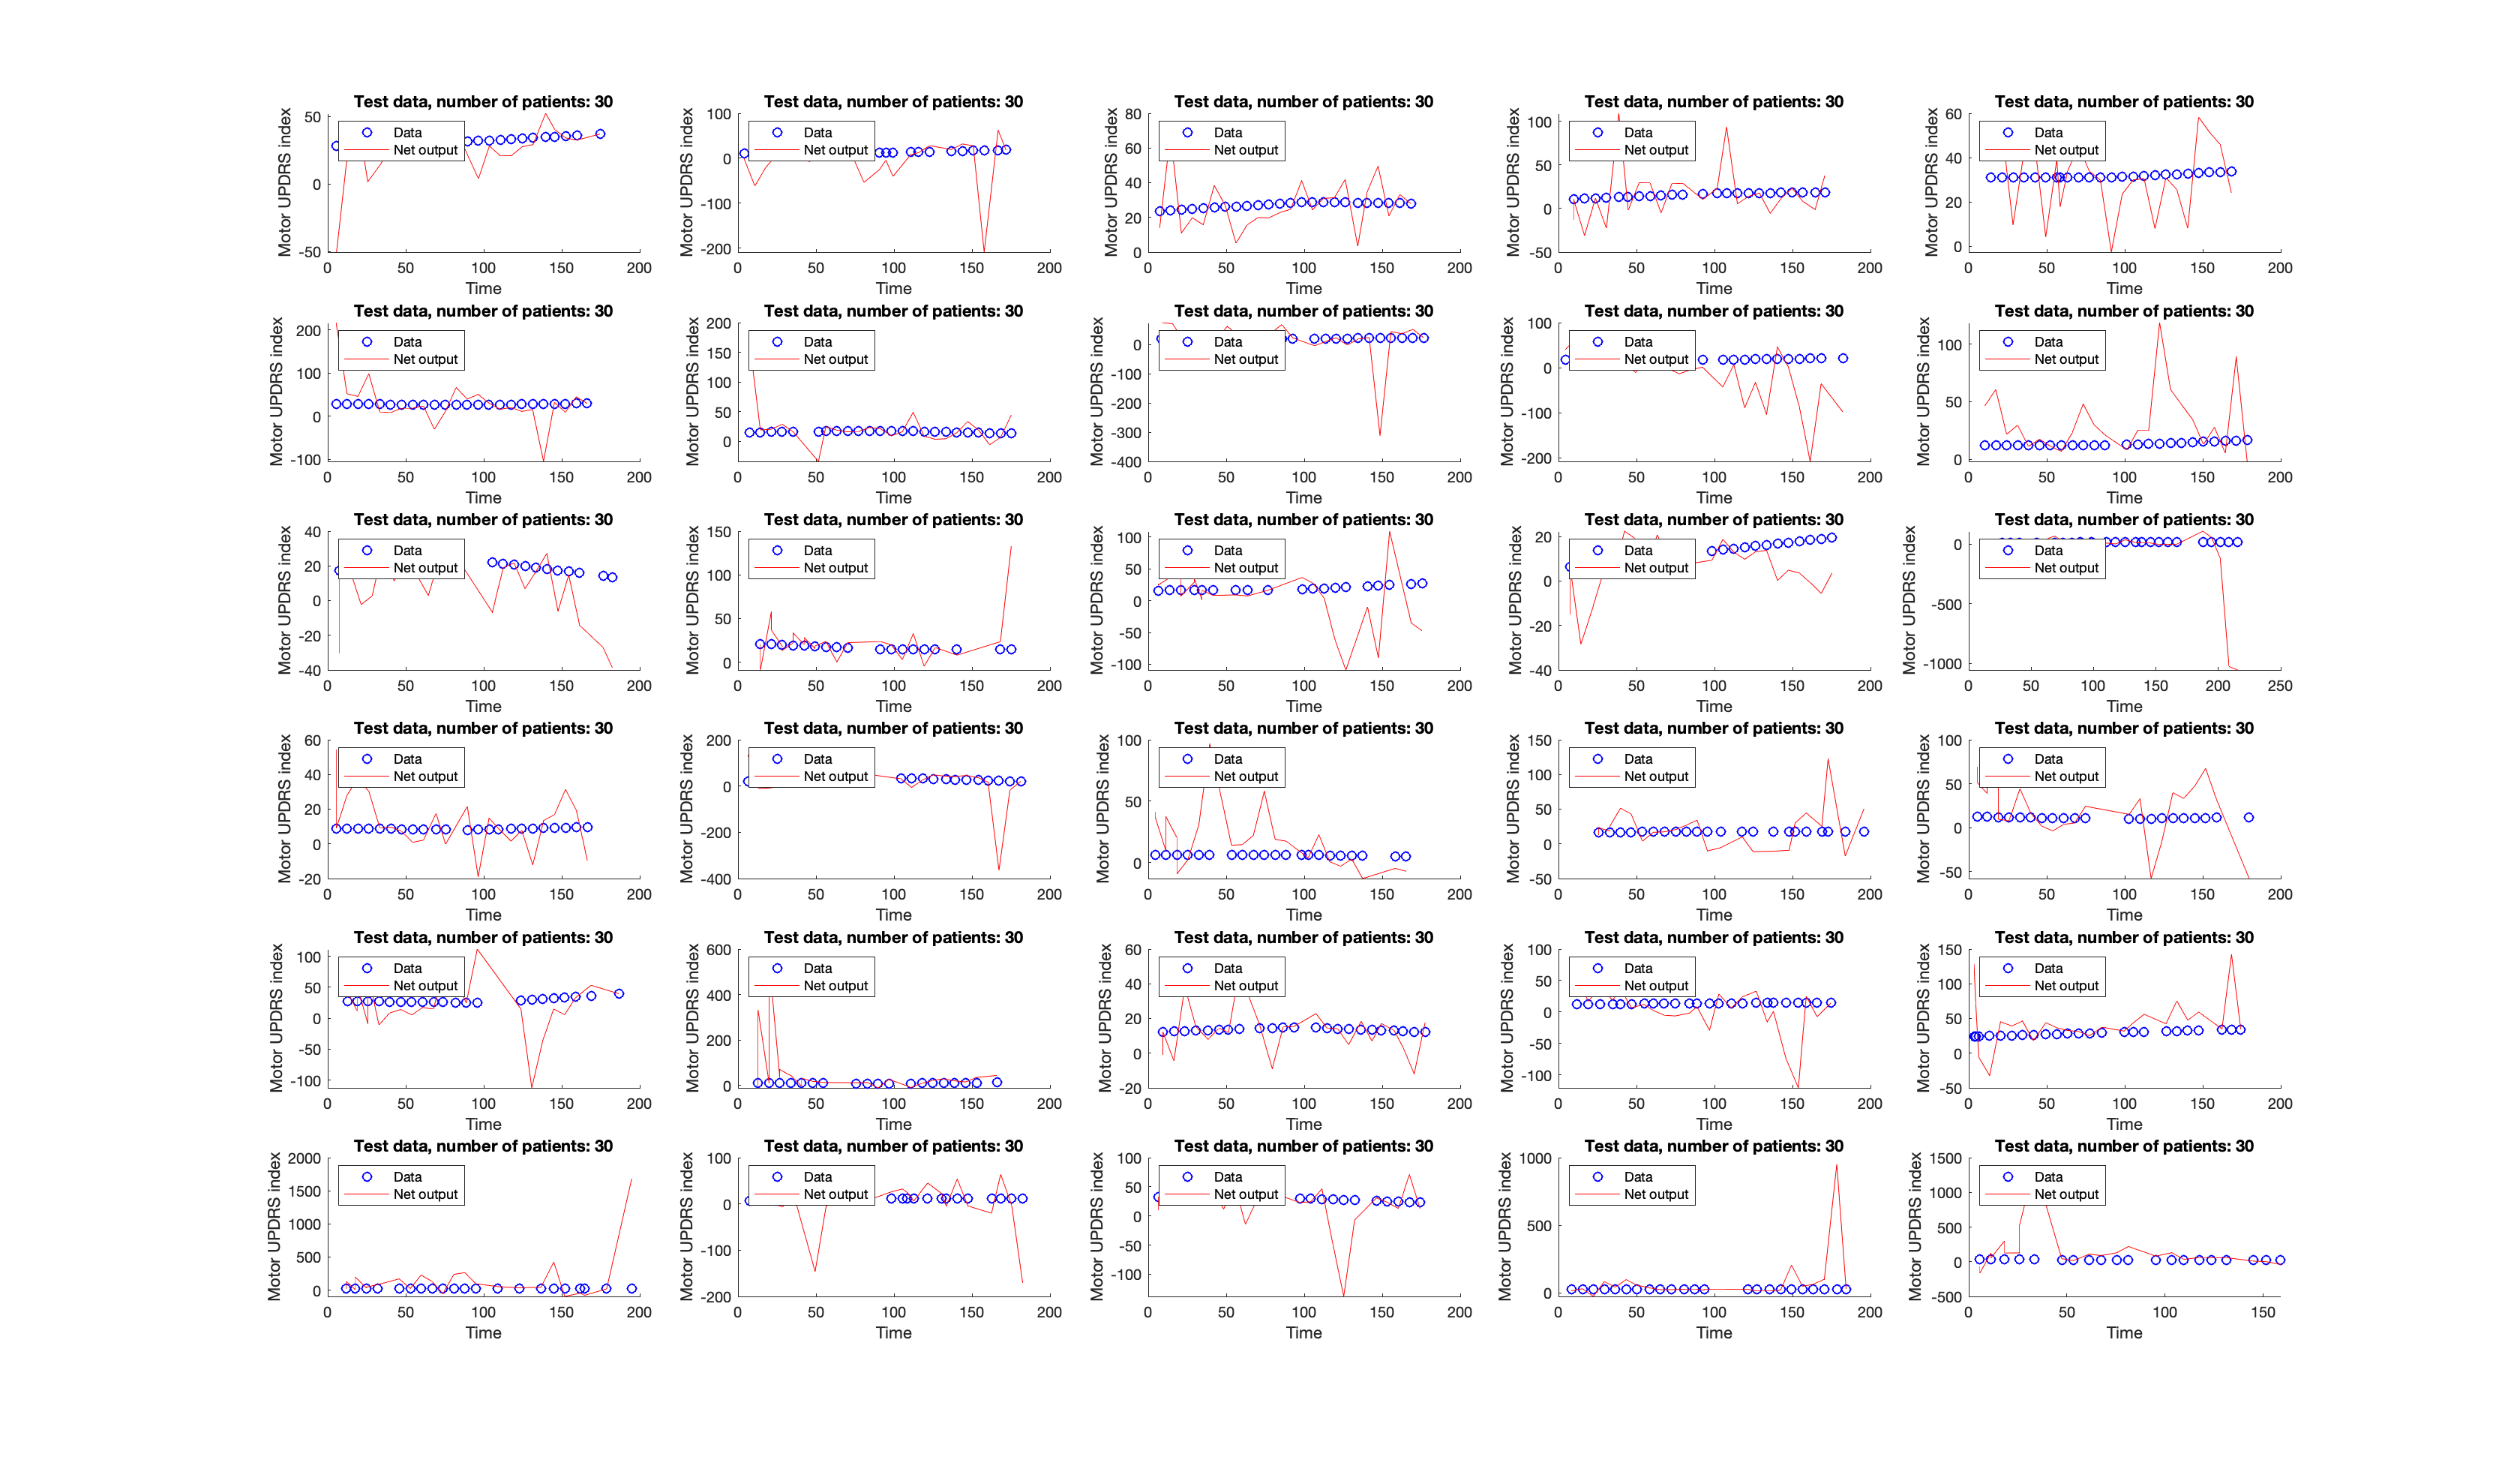
\includegraphics[width=1.00\textwidth]{test-cut-30.png}
\caption{Zbiór testowy, 30 pacjentów}

\end{figure}

\begin{figure}[h!]

\centering
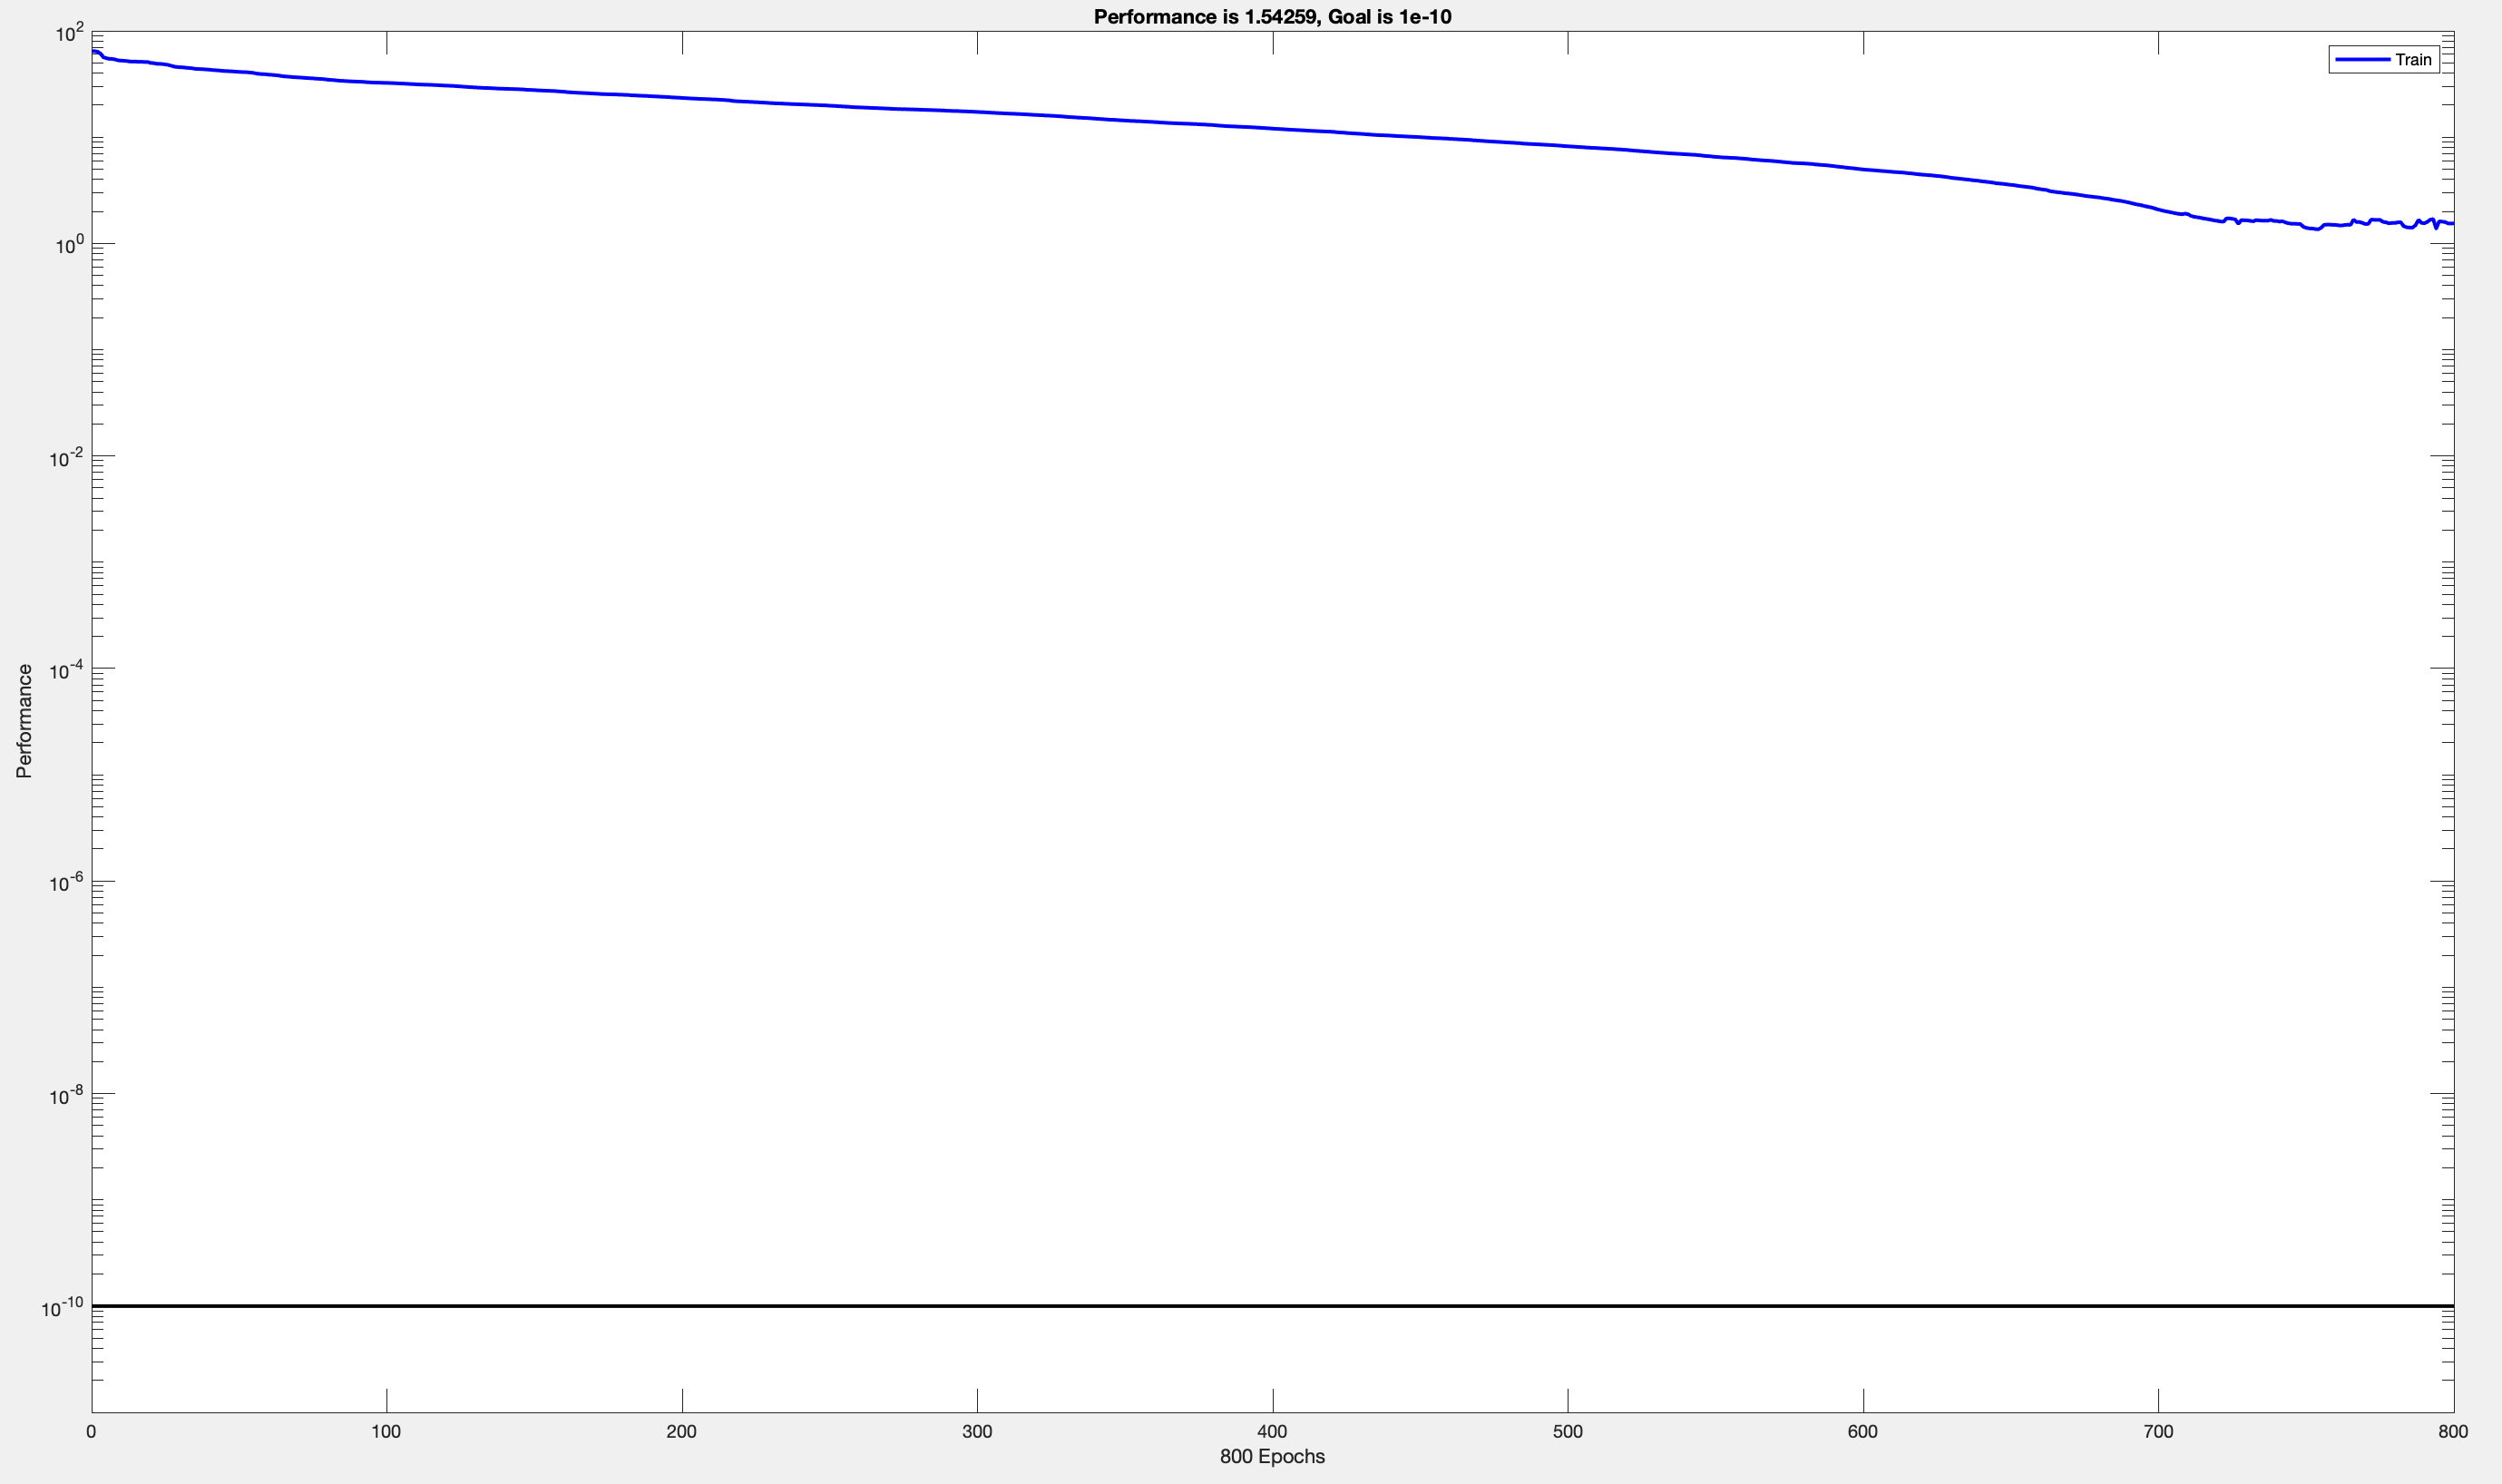
\includegraphics[width=1.0\textwidth]{mse-cut-36.png}
\caption{MSE dla 36 pacjentów}

\end{figure}

\begin{figure}[h!]

\centering
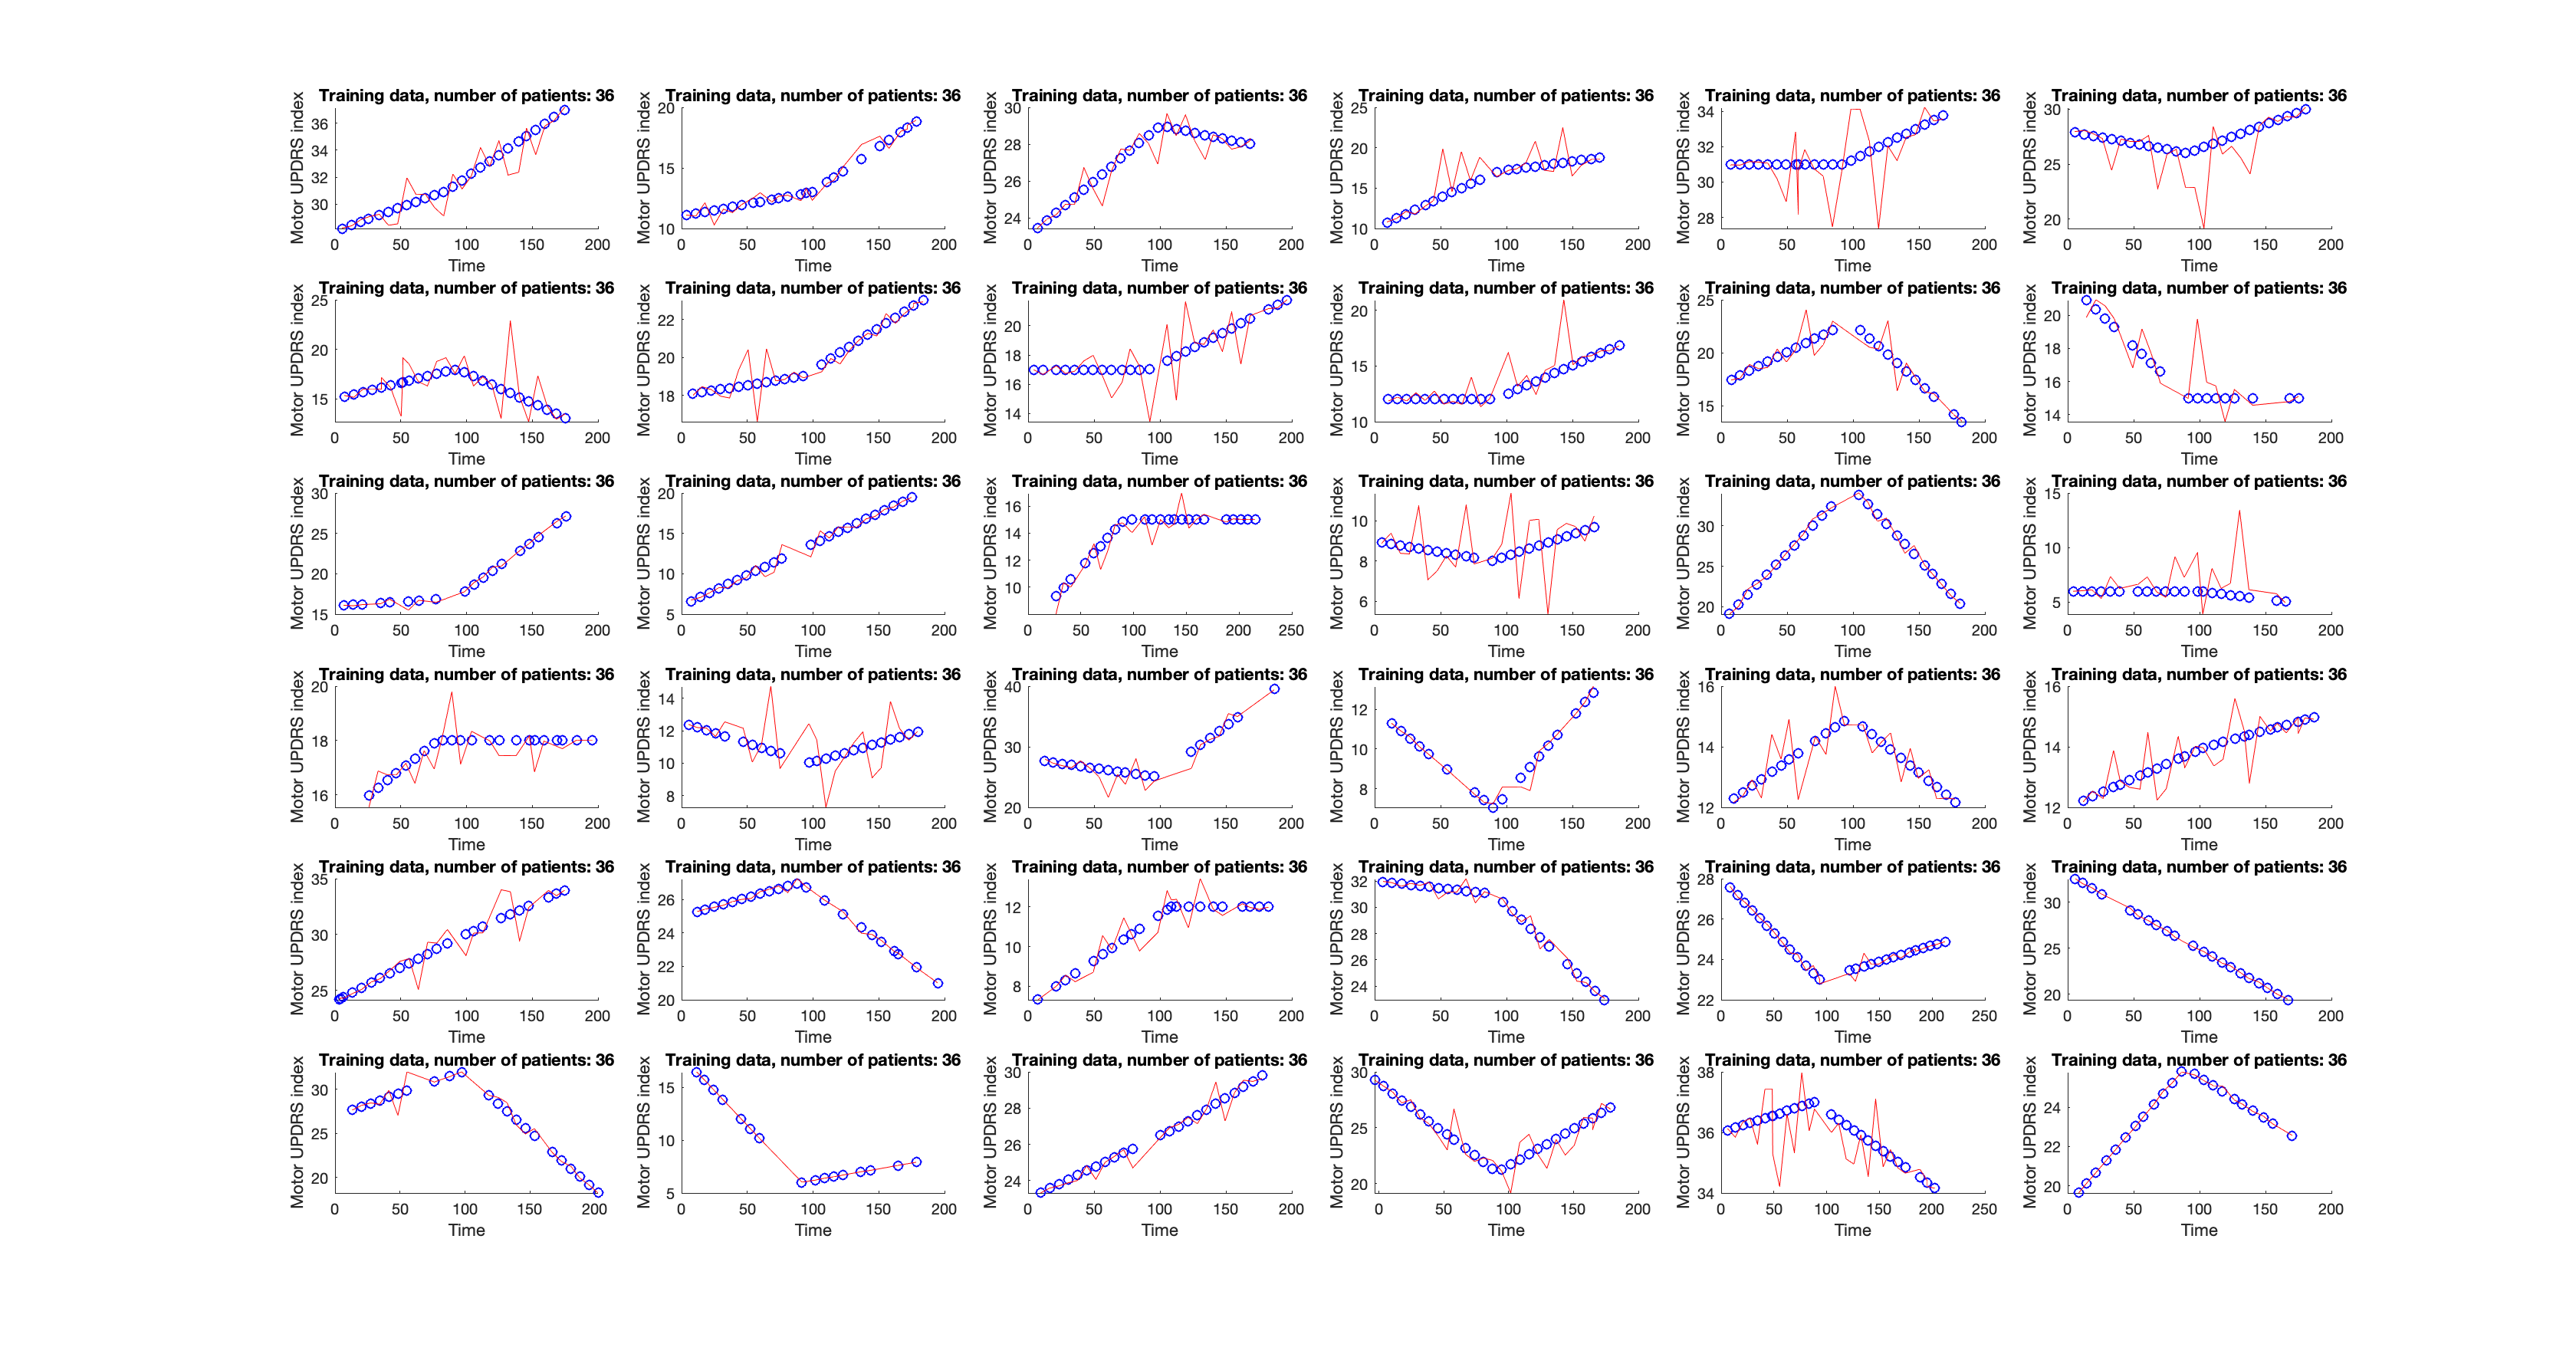
\includegraphics[width=1.1\textwidth]{training-cut-36.png}
\caption{Zbiór treningowy, 36 pacjentów}

\end{figure}

\begin{figure}[h!]

\centering
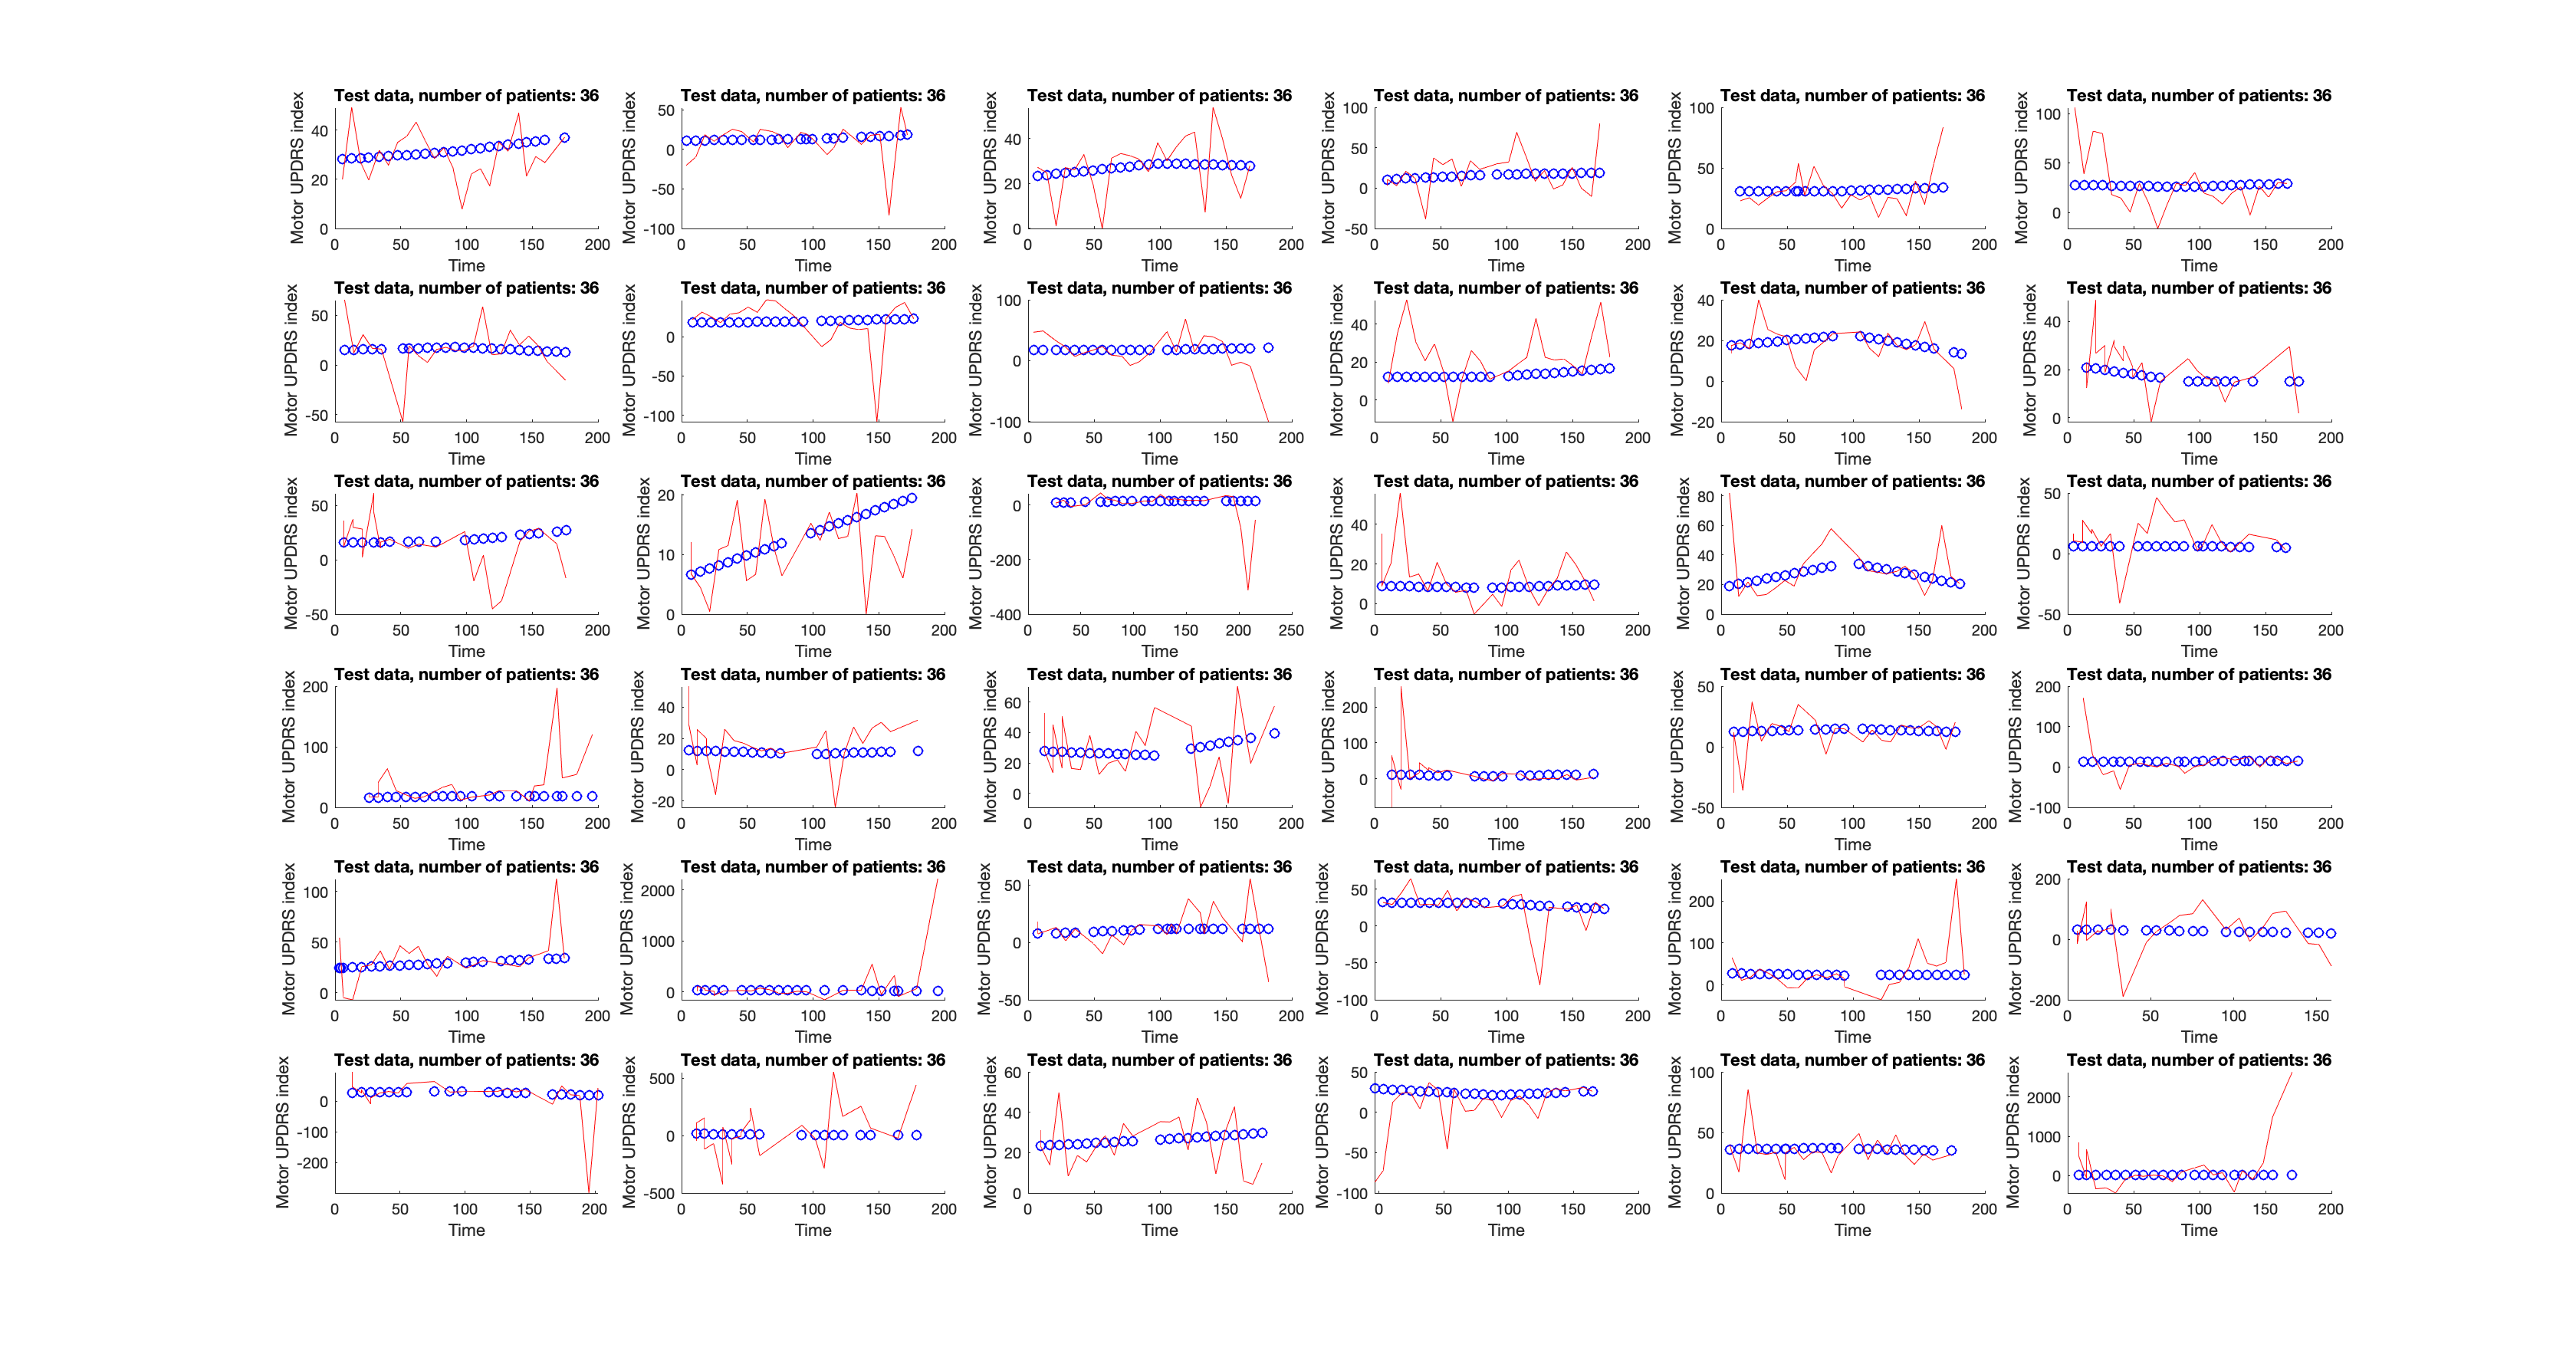
\includegraphics[width=1.1\textwidth]{test-cut-36.png}
\caption{Zbiór testowy, 36 pacjentów}

\end{figure}

\begin{figure}[h!]

\centering
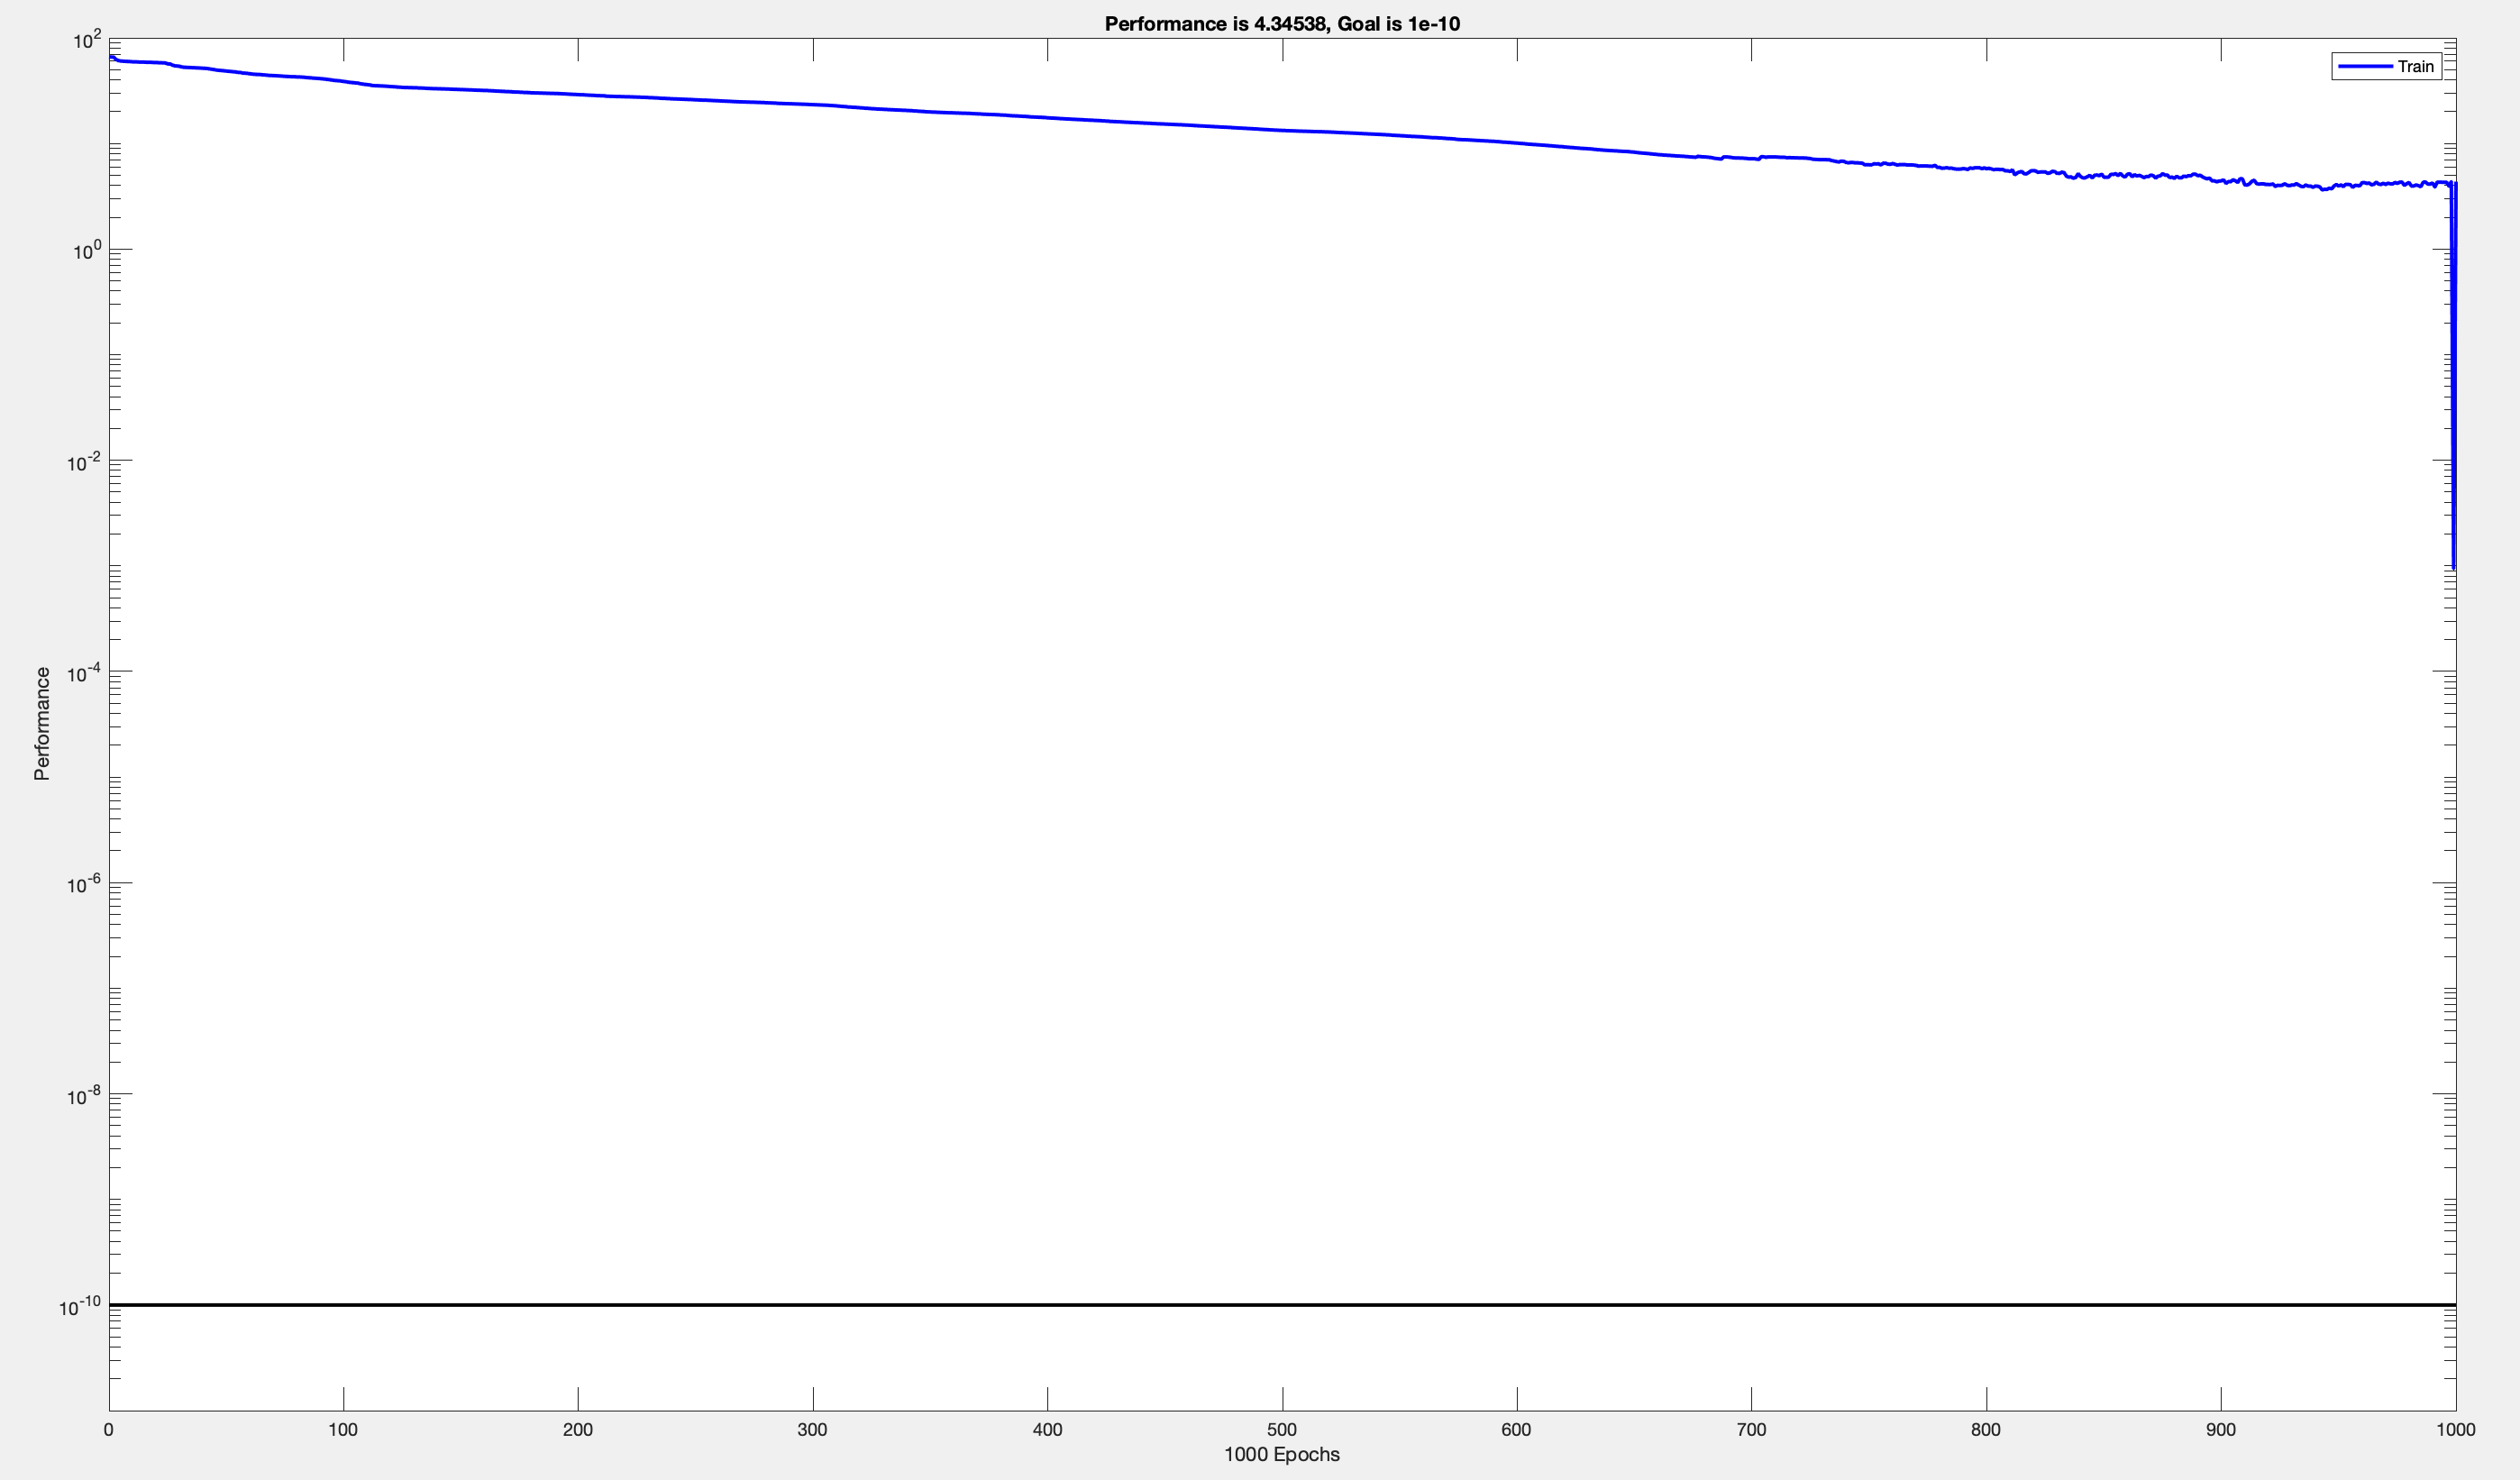
\includegraphics[width=1.0\textwidth]{mse-cut-42.png}
\caption{MSE dla 42 pacjentów}

\end{figure}

\begin{figure}[h!]

\centering
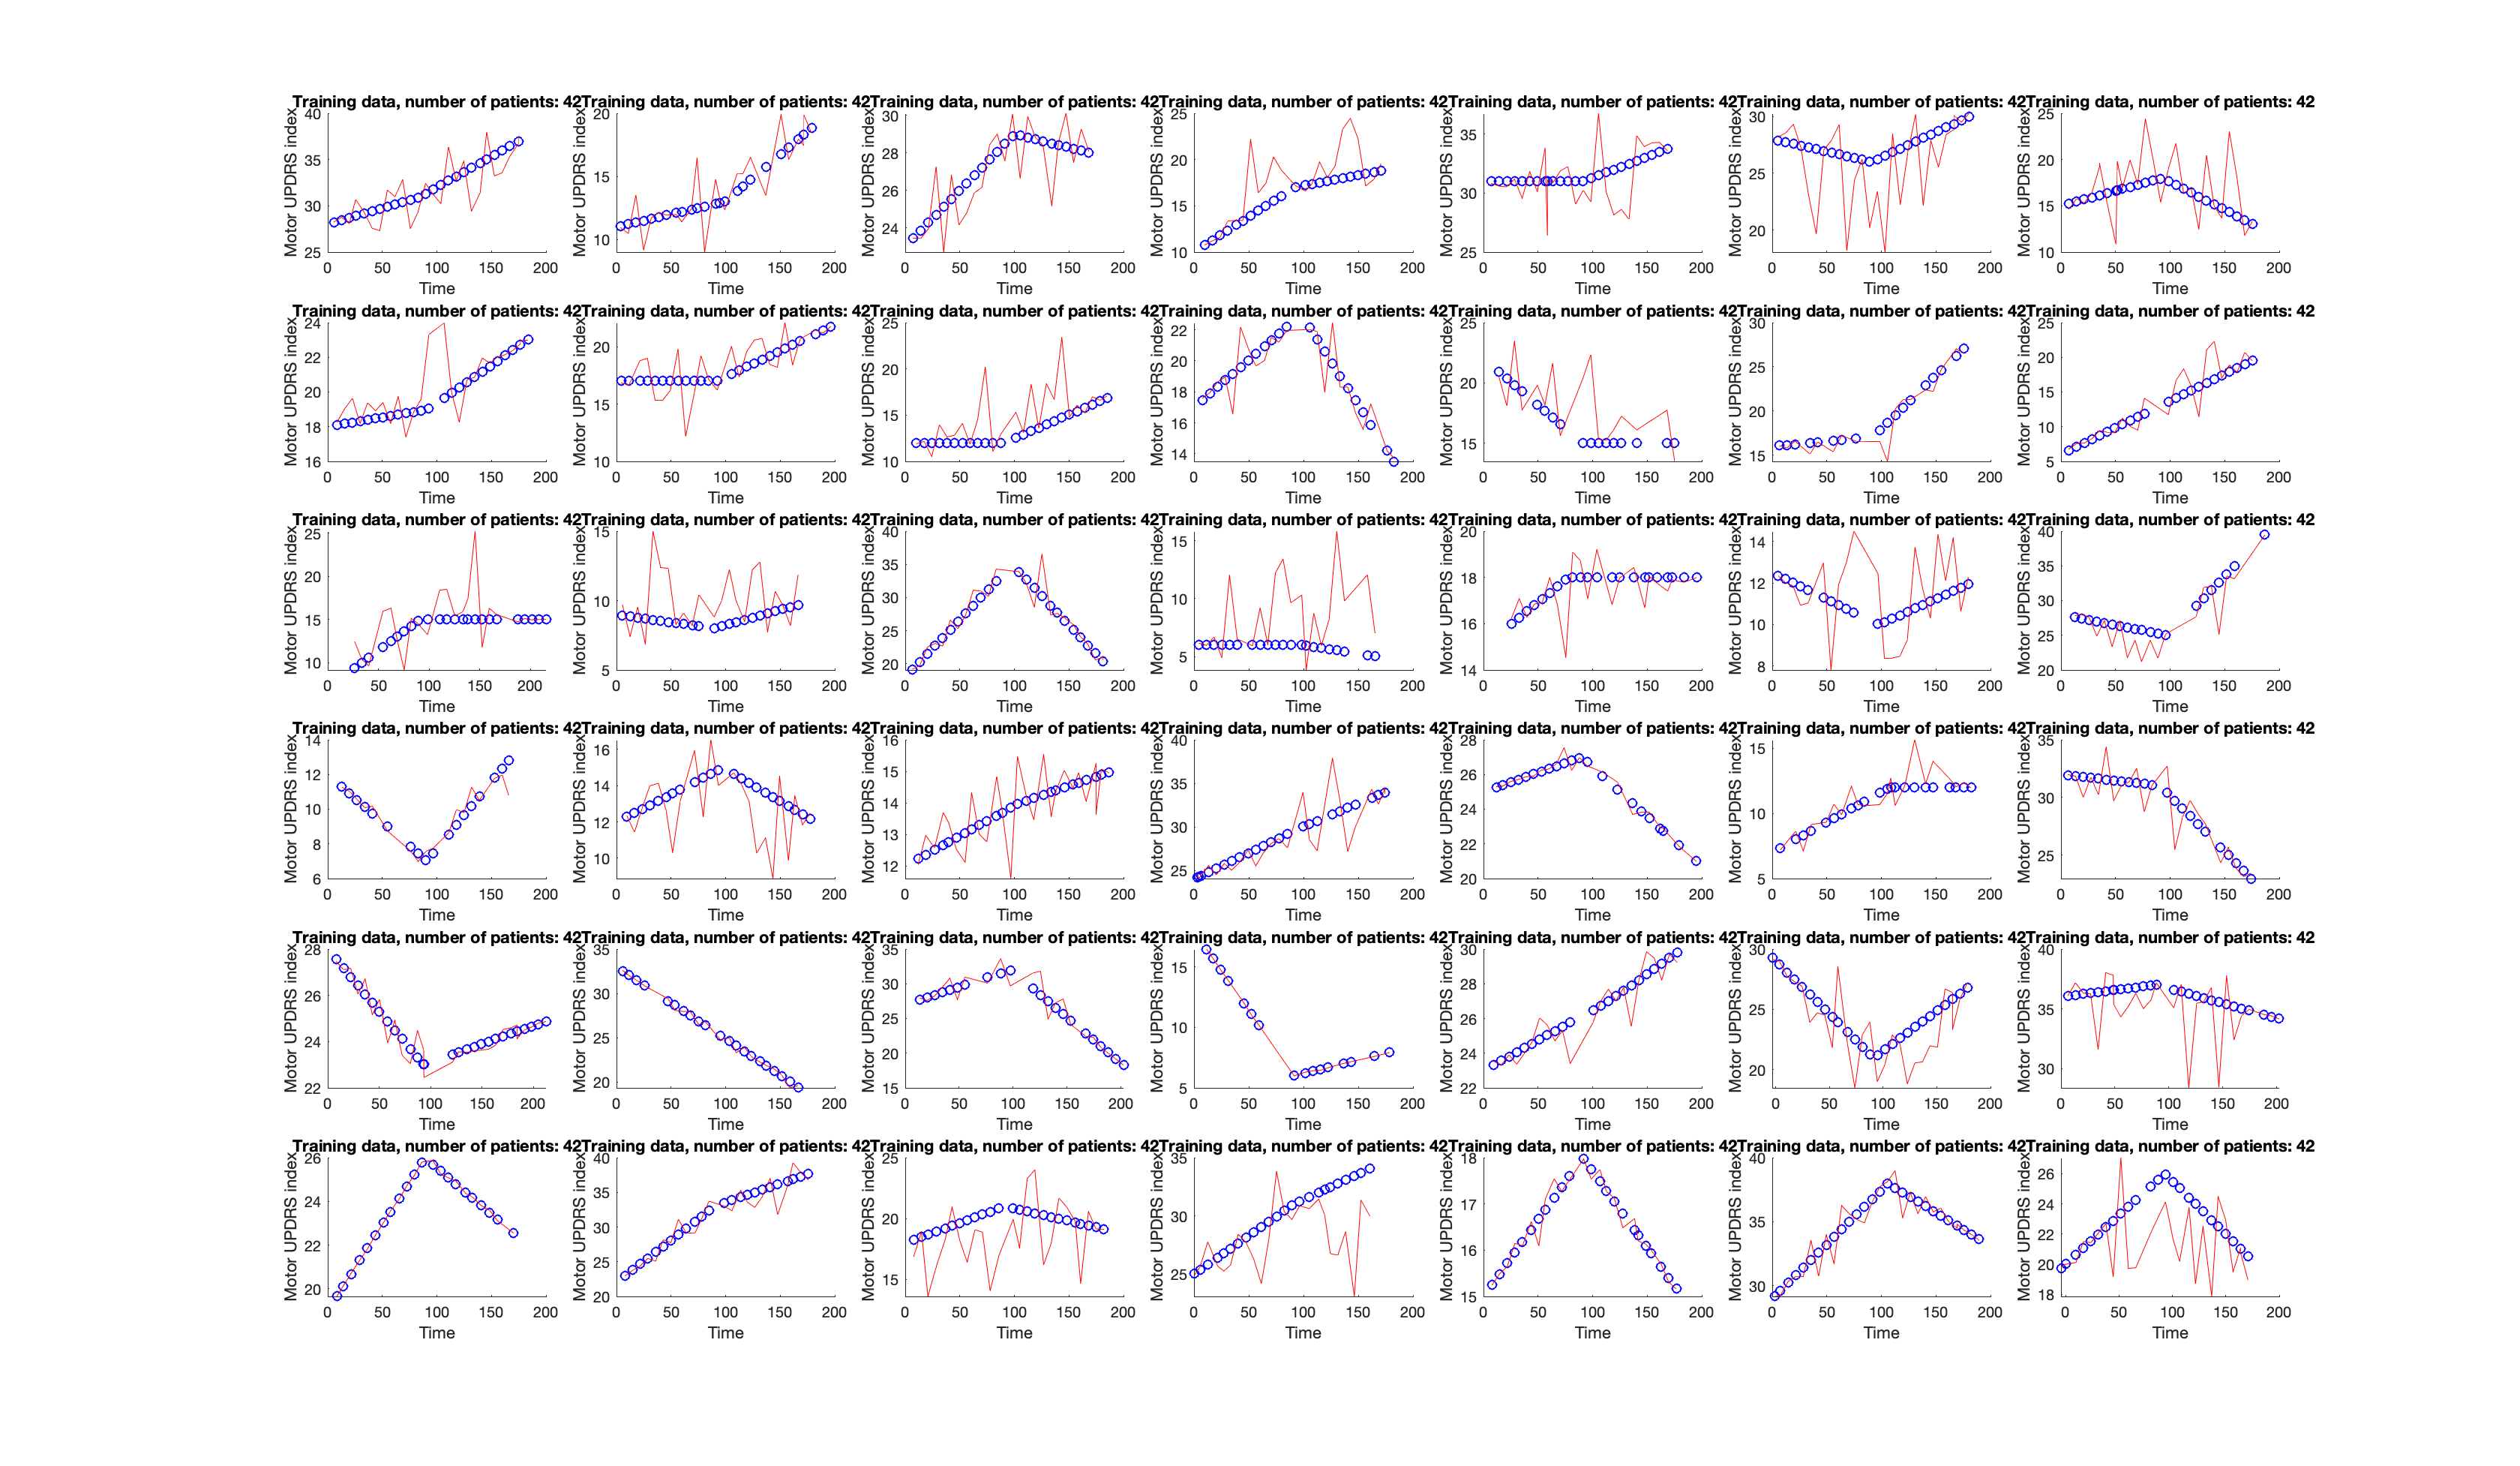
\includegraphics[width=1.0\textwidth]{training-cut-42.png}
\caption{Zbiór treningowy, 42 pacjentów}

\end{figure}

\begin{figure}[h!]

\centering
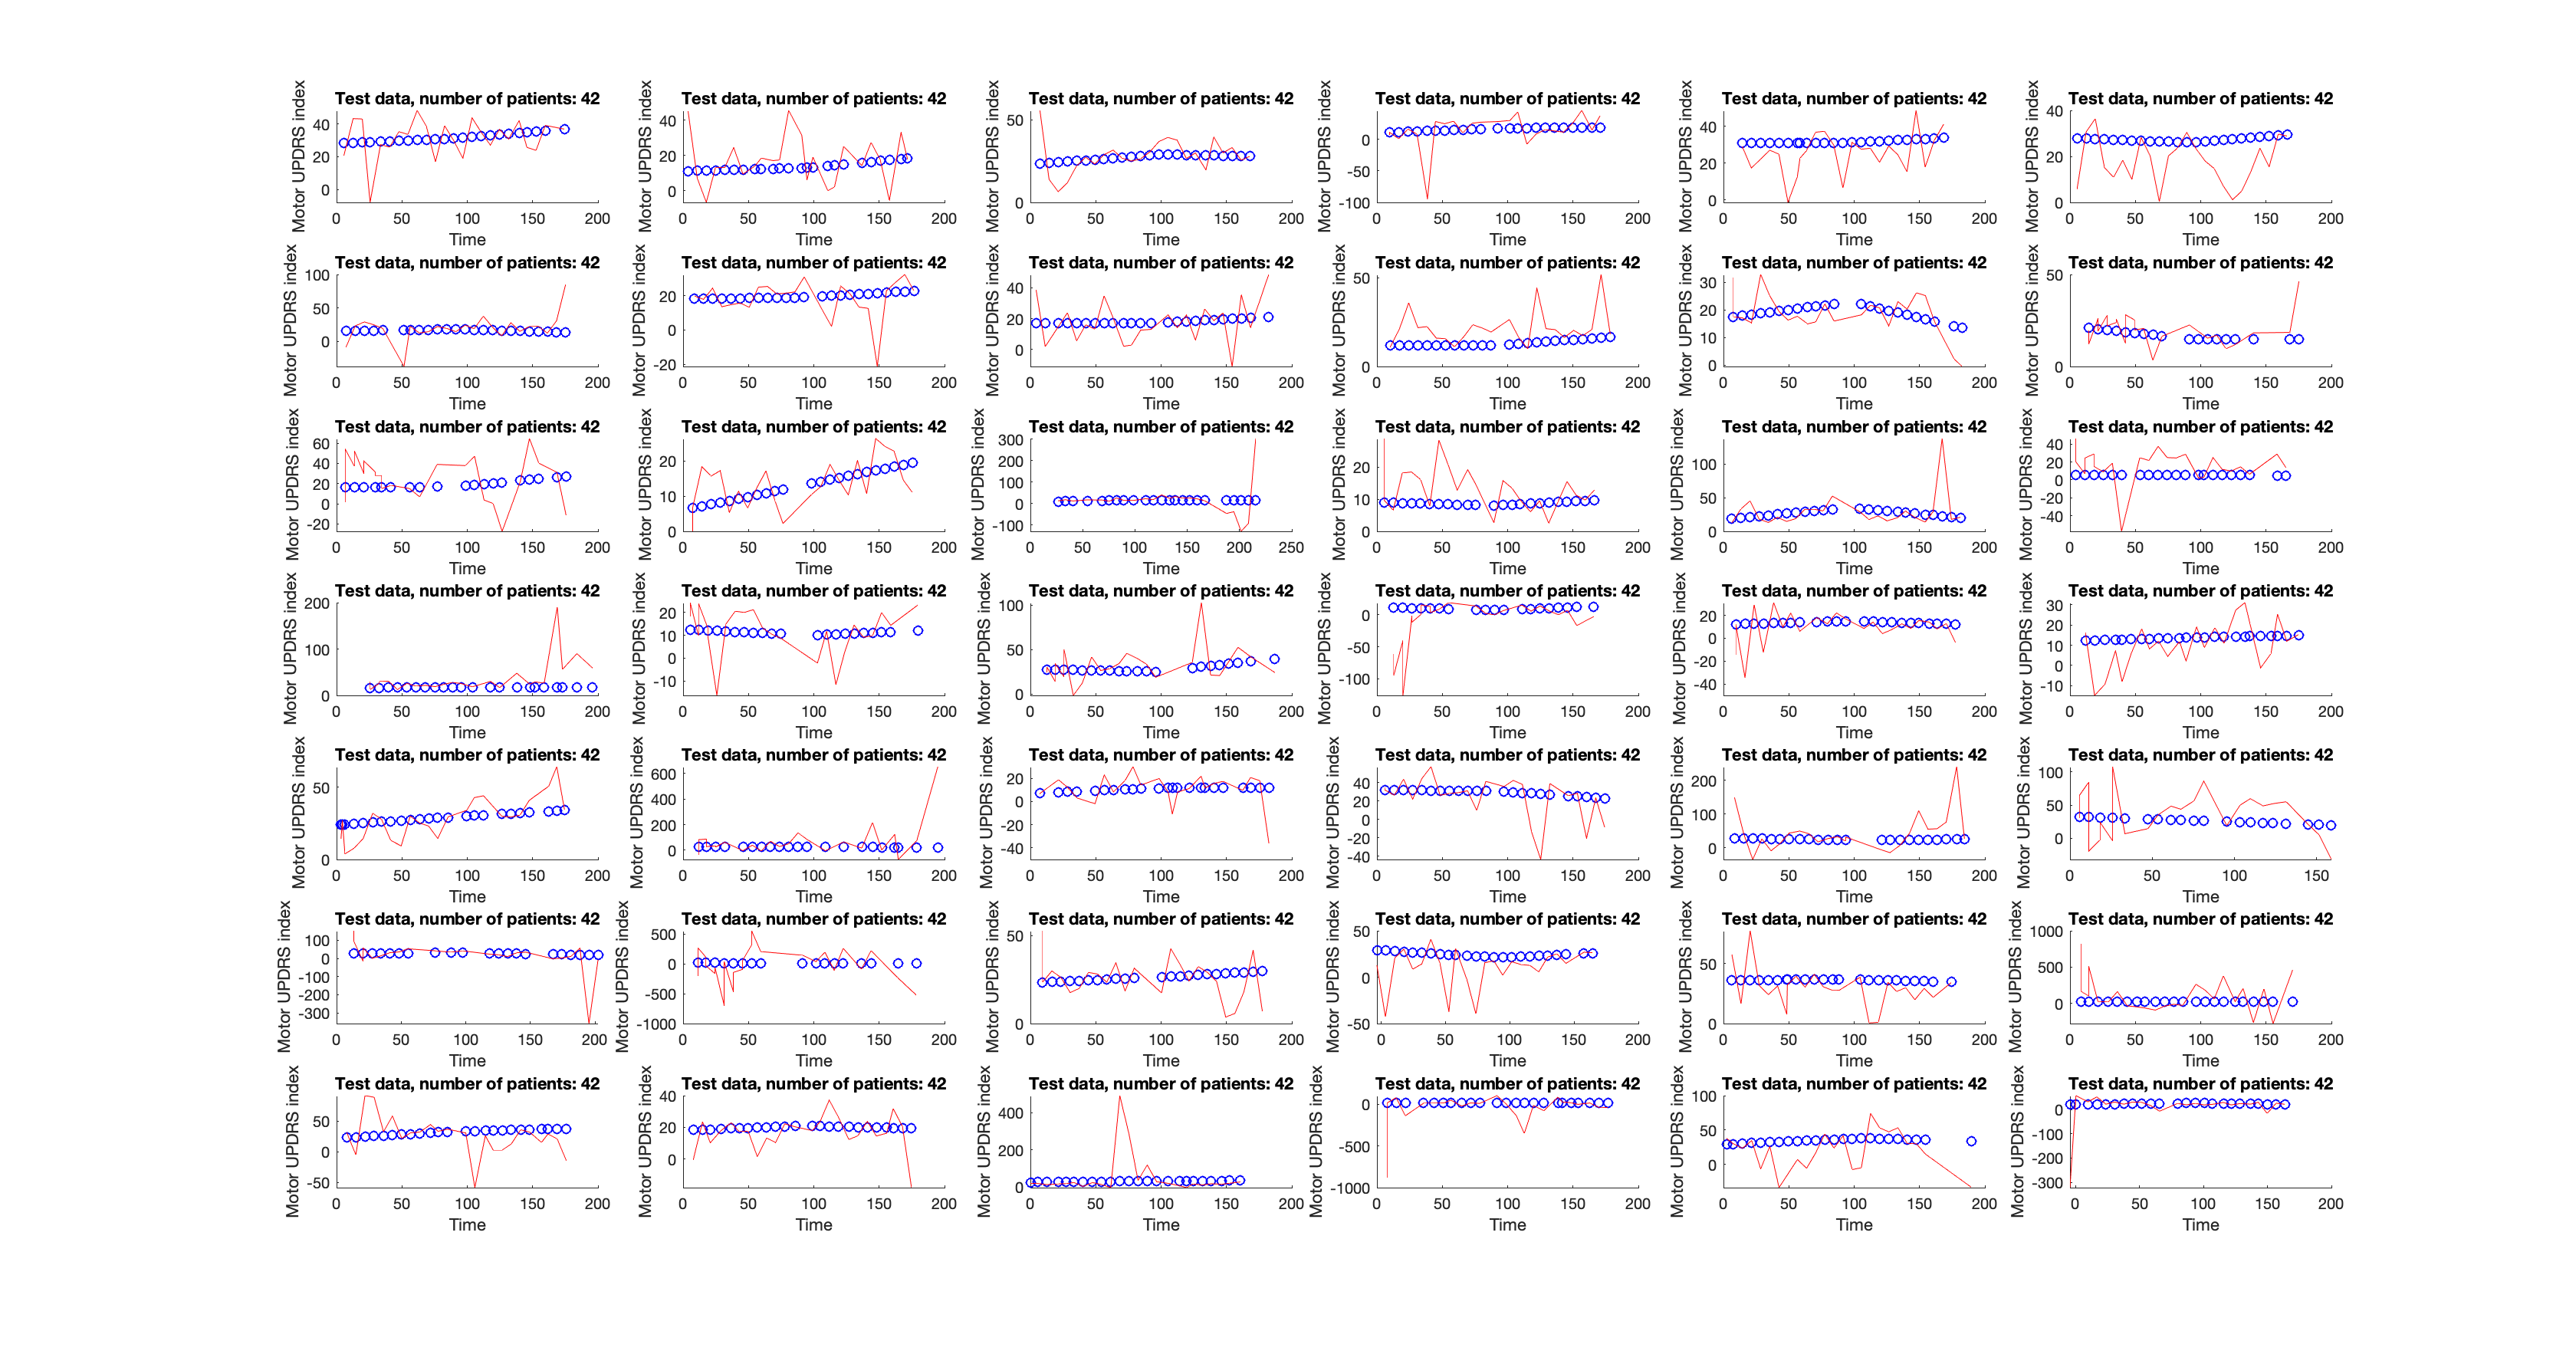
\includegraphics[width=1.1\textwidth]{test-cut-42.png}
\caption{Zbiór testowy, 42 pacjentów}

\end{figure}

Przy zwiększeniu liczby pacjentów dla danych nie zawierających duplikatów widać znaczne poprawienie szybkości nauki oraz dopasowania sieci w~zbiorze testowym, jednak widoczne jest pogłębienie problemów w nauce zbioru uczącego. Nie wszystkie predykcje wykonywane są w pełni poprawnie, ale jest to rekompensowane szybkim czasem uczenia.

\newpage
\section{Wnioski}

\begin{itemize}
\item Sieci radialne bardzo dobrze radzą sobie z zadaniami predykcji dla jednego pacjenta (klasy)
\item Po wprowadzenie wielu pacjentów (klas) sieci radialne wykazują niewielkie problemy w nauce, czego przyczyną może być niskiej jakości zbiór uczący
\item Przy użyciu danych z duplikatami sieć radialna nie ma problemów z~nauką w przypadku małej ilości klas. Czas nauki jest dłuższy niż w przypadku danych bez duplikatów, dopasowanie sieci jest większe.
\item Zwiększając liczbę klas i wykorzystując dane bez duplikatów czas uczenia osiąga duże wartości. Nie jest możliwa wizualizacja wyników dla maksymalnej liczby pacjentów.
\item Przy użyciu danych bez duplikatów szybkość uczenia sieci radialnej znacząco maleje, umożliwiając w ten sposób wizualizację wyników dla maksymalnej liczby klas
\end{itemize}

\newpage
\begin{thebibliography}{9}

\bibitem{zbioruczacy}
A Tsanas, MA Little, PE McSharry, LO Ramig (2009) 
'Accurate telemonitoring of Parkinson’s disease progression by non-invasive speech tests', 
IEEE Transactions on Biomedical Engineering (to appear). 
\\\texttt{https://archive.ics.uci.edu/ml/datasets/Parkinsons+\\Telemonitoring}

\bibitem{zbior-uczacy1}
Little MA, McSharry PE, Hunter EJ, Ramig LO (2009), 
'Suitability of dysphonia measurements for telemonitoring of Parkinson's disease', 
IEEE Transactions on Biomedical Engineering, 56(4):1015-1022 

\bibitem{zbior-uczacy2}
Little MA, McSharry PE, Roberts SJ, Costello DAE, Moroz IM. 
'Exploiting Nonlinear Recurrence and Fractal Scaling Properties for Voice Disorder Detection', 
BioMedical Engineering OnLine, 26 June 2007

\bibitem{Osowski ujecie algorytmiczne}
Stanisław Osowski.
\textit{Sieci Neuronowe w ujęciu algorytmicznym}
Wydawnictwo Naukowo-Techniczne, Warszawa 1996

\bibitem{Osowski przetwarzanie informacji}
Stanisław Osowski.
\textit{Sieci Neuronowe do przetwarzania informacji}
Oficyna Wydawnicza Politechniki Warszawskiej, Warszawa 2006

\bibitem{Spread Constant}
Hongfa Wang, Xinai Xu, Zhejiang
Water Conservancy and Hydropower College
Determination of Spread Constant in RBF Neural Network by Genetic
Algorithm 
\textit{http://www.globalcis.org/ijact/ppl/IJACT3017PPL.pdf}

\bibitem{matlab}
Oficjalna dokumentacja Mathworks Deep Learning Toolbox. 
\\\texttt{https://www.mathworks.com/help/deeplearning/examples/radial-\\basis-approximation.html}

\bibitem{owards Data Sience}
Towards Data Science blog
\\\texttt{https://towardsdatascience.com/radial-basis-functions-neural-\\networks-all-we-need-to-know-9a88cc053448}


\end{thebibliography}
\newpage

\listoffigures
\newpage

\end{document}